%% 
%% Copyright 2007-2026 Elsevier Ltd
%% 
%% This file is part of the 'Elsarticle Bundle'.
%% ---------------------------------------------
%% 
%% It may be distributed under the conditions of the LaTeX Project Public
%% License, either version 1.3 of this license or (at your option) any
%% later version.  The latest version of this license is in
%%    http://www.latex-project.org/lppl.txt
%% and version 1.3 or later is part of all distributions of LaTeX
%% version 1999/12/01 or later.
%% 
%% The list of all files belonging to the 'Elsarticle Bundle' is
%% given in the file `manifest.txt'.
%% 
%% Template article for Elsevier's document class `elsarticle'
%% with numbered style bibliographic references
%% SP 2008/03/01
%% $Id: elsarticle-template-num.tex 289 2026-01-09 06:13:01Z rishi $
%%
\documentclass[preprint,12pt]{elsarticle}

%% Use the option review to obtain double line spacing
%% \documentclass[authoryear,preprint,review,12pt]{elsarticle}

%% Use the options 1p,twocolumn; 3p; 3p,twocolumn; 5p; or 5p,twocolumn
%% for a journal layout:
%% \documentclass[final,1p,times]{elsarticle}
%% \documentclass[final,1p,times,twocolumn]{elsarticle}
%% \documentclass[final,3p,times]{elsarticle}
%% \documentclass[final,3p,times,twocolumn]{elsarticle}
%% \documentclass[final,5p,times]{elsarticle}
%% \documentclass[final,5p,times,twocolumn]{elsarticle}

%% For including figures, graphicx.sty has been loaded in
%% elsarticle.cls. If you prefer to use the old commands
%% please give \usepackage{epsfig}

%% The amssymb package provides various useful mathematical symbols
\usepackage{amssymb}
%% The amsmath package provides various useful equation environments.
\usepackage{amsmath}
%% The amsthm package provides extended theorem environments
%% \usepackage{amsthm}

%% The lineno packages adds line numbers. Start line numbering with
%% \begin{linenumbers}, end it with \end{linenumbers}. Or switch it on
%% for the whole article with \linenumbers.
%% \usepackage{lineno}
\usepackage{booktabs}
\usepackage{xurl}
\usepackage{multirow}
\usepackage{array}
\newcolumntype{C}[1]{>{\centering\arraybackslash}p{#1}}
\journal{Computer Methods in Applied Mechanics and Engineering}

\begin{document}

\begin{frontmatter}

%% Title, authors and addresses

%% use the tnoteref command within \title for footnotes;
%% use the tnotetext command for theassociated footnote;
%% use the fnref command within \author or \affiliation for footnotes;
%% use the fntext command for theassociated footnote;
%% use the corref command within \author for corresponding author footnotes;
%% use the cortext command for theassociated footnote;
%% use the ead command for the email address,
%% and the form \ead[url] for the home page:
%% \title{Title\tnoteref{label1}}
%% \tnotetext[label1]{}
%% \author{Name\corref{cor1}\fnref{label2}}
%% \ead{email address}
%% \ead[url]{home page}
%% \fntext[label2]{}
%% \cortext[cor1]{}
%% \affiliation{organization={},
%%             addressline={},
%%             city={},
%%             postcode={},
%%             state={},
%%             country={}}
%% \fntext[label3]{}

\title{Efficient GPU-Accelerated ADMM for Large-Scale Lower-Bound Finite Element Limit Analysis}

%% use optional labels to link authors explicitly to addresses:
%% \author[label1,label2]{}
%% \affiliation[label1]{organization={},
%%             addressline={},
%%             city={},
%%             postcode={},
%%             state={},
%%             country={}}
%%
%% \affiliation[label2]{organization={},
%%             addressline={},
%%             city={},
%%             postcode={},
%%             state={},
%%             country={}}

\author{Yunfei Gao, Chris Martin, Paul Goulart} %% Author name

%% Author affiliation
\affiliation{organization={Department of Engineering Science, University of Oxford},%Department and Organization
            addressline={Parks Road}, 
            city={Oxford},
            postcode={OX1 3PJ}, 
            state={Oxfordshire},
            country={UK}}

%% Abstract
\begin{abstract}
%% Text of abstract


We propose a GPU-accelerated alternating direction method of multipliers (ADMM) framework for solving large-scale lower-bound (LB) finite element limit analysis (FELA) problems. The method incorporates active-cone identification with dynamic penalty reweighting, as well as a coarse-to-fine continuation strategy that exploits ADMM’s warm-start capability to improve convergence on large, sparse conic optimization problems. The dominant sparse linear solves and vector operations are implemented on the GPU using CUDA, significantly reducing per-iteration cost. The proposed framework is systematically evaluated on large-scale 2D and 3D FELA benchmarks formulated as second-order cone programming (SOCP) problems, where it demonstrates substantial speedups over a  commercial interior-point solver while maintaining comparable accuracy. In addition, we demonstrate that the same framework extends naturally to representative 3D FELA problems. These results indicate that GPU-accelerated ADMM provides an efficient and extensible approach for large-scale FELA, combining strong performance in 2D with practical applicability to 3D problems.


\end{abstract}

%%Graphical abstract
\begin{graphicalabstract}
%\includegraphics{grabs}

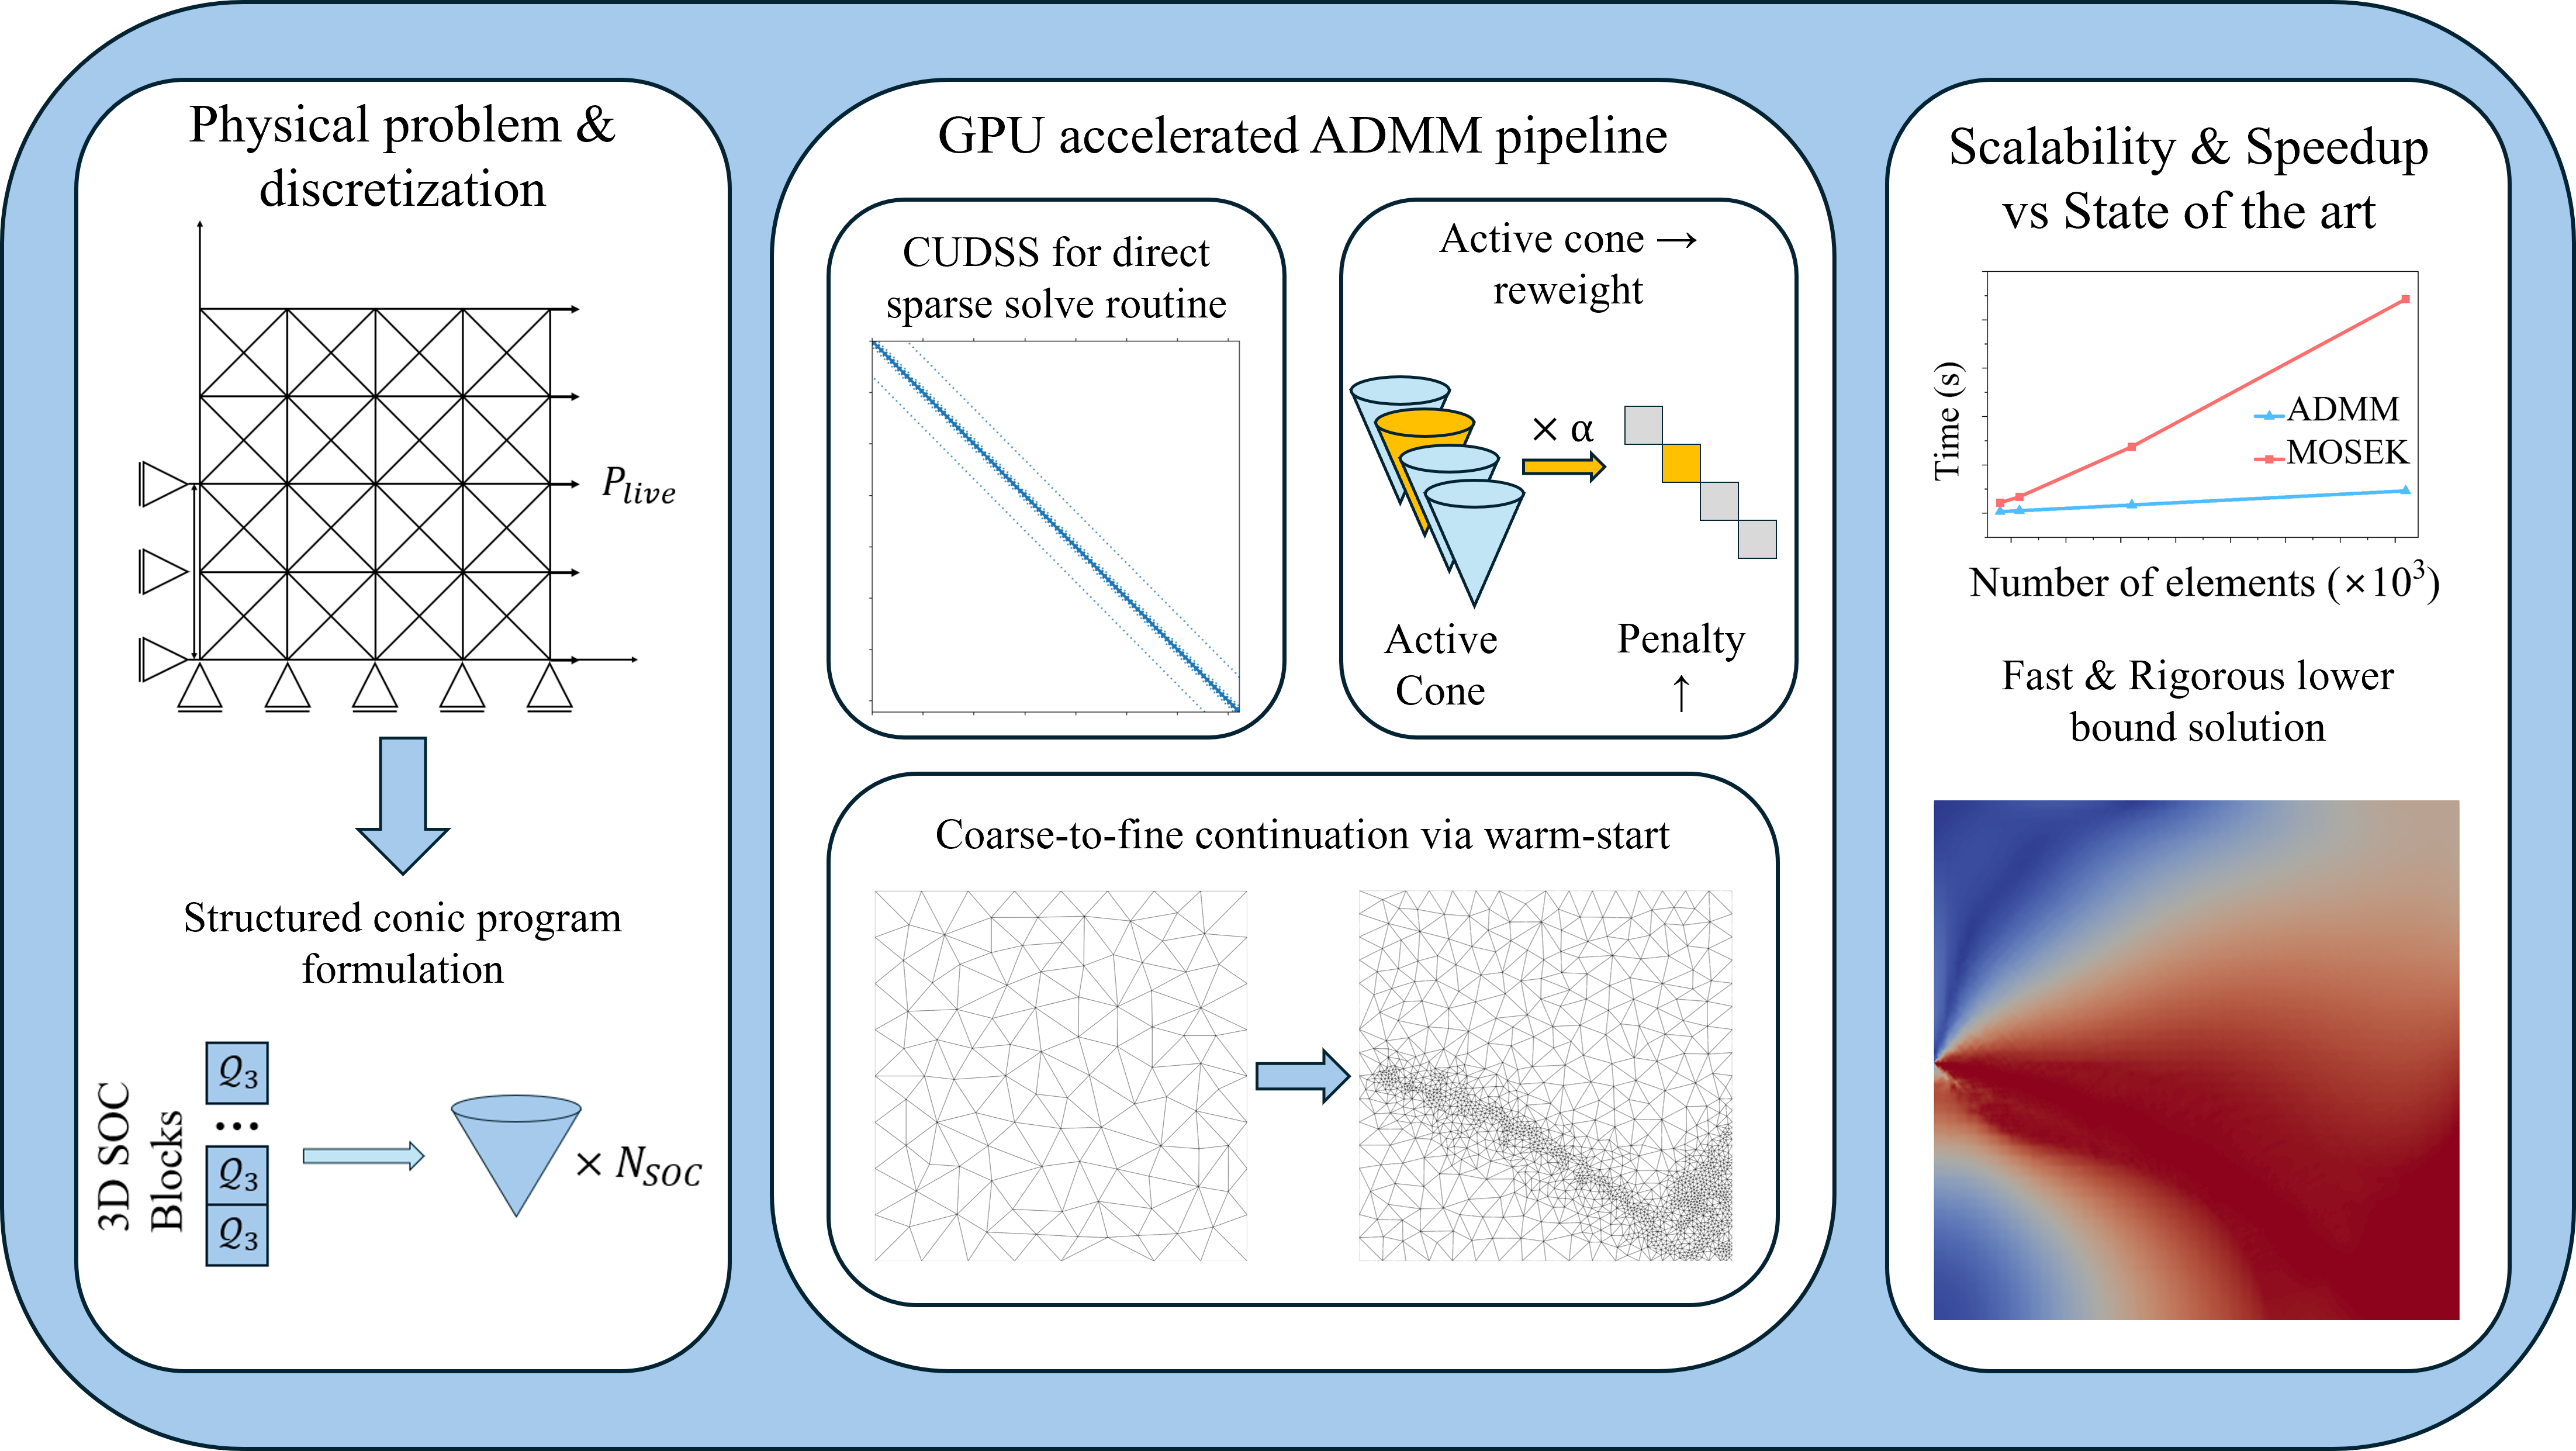
\includegraphics[width=1.0\textwidth]{figures/Res_To_Date/GA.png} 
\end{graphicalabstract}

%%Research highlights
\begin{highlights}
\item  GPU-accelerated ADMM pipeline for million-variable LB-FELA SOCPs, outperforming IPM baselines in time-to-solution while preserving accuracy. 

\item Active-cone identification and dynamic penalty reweighting for SOC blocks to accelerate convergence in block-structured SOCPs. 

\item Coarse-to-fine continuation with warm starts across mesh resolutions, substantially reducing iteration counts for the same benchmark under finer mesh discretizations.

\item GPU linear-solve and projection kernels with symbolic factorization reuse, enabling efficient large-scale computations.






\end{highlights}

%% Keywords
\begin{keyword}
%% keywords here, in the form: keyword \sep keyword
Alternating direction of multipliers method \sep Finite element limit analysis \sep Second-order cone programming \sep GPU computing
%% PACS codes here, in the form: \PACS code \sep code

%% MSC codes here, in the form: \MSC code \sep code
%% or \MSC[2008] code \sep code (2000 is the default)

\end{keyword}

\end{frontmatter}

%% Add \usepackage{lineno} before \begin{document} and uncomment 
%% following line to enable line numbers
%% \linenumbers

%% main text
%%



\section{Introduction}

%FELA in general
% 2.0: FELA introduction and we only focus on LB in this paper.

%The determination of the ultimate load-carrying capacity, or collapse load, of geotechnical structures is a fundamental task in stability analysis and design. Finite Element Limit Analysis (FELA) provides a rigorous numerical framework for this purpose by computing strict upper and lower bounds to the true collapse load~\cite{Sloan_stability_analysis, Dunne_thesis}. This paper focuses on lower-bound FELA, where the objective is to construct a statically admissible stress field that satisfies equilibrium, boundary conditions, and yield admissibility.


% Convex failure criteria, converts the problem to cvxopt problems.
% 2.0: LB FELA in 2D and 3D leads to large-scale SOCPs and even SDPs.

%For many convex yield criteria, the lower-bound FELA formulation can be cast as a conic optimization problem. In 2D, criteria such as Tresca and Mohr-Coulomb can be represented using second-order cone (SOC) constraints, leading to Second-Order Cone Programming (SOCP) formulations~\cite{2DLB, UB_simplex}. Similar SOCP structures also arise in selected three-dimensional formulations, for example with von Mises or Drucker-Prager criteria, while other yield criteria may require semidefinite or nonlinear programming representations~\cite{3DLB, 3DLD, 3DHB, 3DBishop}. When Bernstein polynomial stress elements and adaptive mesh refinement are employed~\cite{Bernstein_FELA}, the resulting discretized problems involve solving optimization problems with an increasing number of linear equilibrium constraints and local yield constraints. For the Drucker-Prager criterion, these yield constraints can be represented as SOC constraints, producing large-scale SOCPs that demand scalable numerical solvers.

% IPM used to be the solver of choice for the past 2 decades.

%For the past decades, the Interior Point Method (IPM) has been the method of choice to solve these problems. However, the IPM theoretically suffers from scalability issues because it needs to reformulate, and refactorize the Karush-Kuhn-Tucker (KKT) matrix in every iteration. Although the development of bespoke, high-performance IPM solvers—exploiting problem structure and GPU parallelism—has alleviated some of these challenges, and such solvers may outperform the state-of-the-art commercial solver MOSEK~\cite{MOSEK, MOSEK_PD, high_performance_IPM} in certain cases, the fundamental limitations of IPMs remain significant in large-scale applications. 

%In the 2010s, several efficient conic solvers were developed for SOCPs based on primal-dual interior-point methods. CVXOPT adopts a dense linear algebra approach using self-dual embedding and Cholesky factorization of the reduced KKT system~\cite{CVXOPT}, while ECOS employs Mehrotra’s predictor-corrector strategy with Nesterov–Todd scaling, using sparse $LDL^\top$ factorization and fixed symbolic ordering for better performance on embedded systems and small problems~\cite{ECOS}.

% Primal-dual IPM algorithms.

%Among some most recent implementations of primal-dual interior point methods, Clarabel is an open-source general purpose solver that solves conic optimization problems, with supported cone types including the second-order cone and exponential cone. It incorporated recent algorithmic advancements including homogeneous embedding and Nesterov-Todd (NT) scaling, allowing it to outperform existing IPM solvers in a series of benchmarks~\cite{Clarabel}. It also comes with a GPU implementation, CuClarabel, utilizing the SIMD (single instruction, multiple data) structure of the GPU to accelerate their IPM method~\cite{CuClarabel}. 


%In recent years, tailored solvers designed for FELA have also been developed. Podlich developed a tailored high-performance interior-point solver that explicitly forms and factorizes the Schur complement system arising in IPM~\cite{high_performance_IPM}. To reduce fill-in and improve numerical efficiency, effective presolve techniques such  as matrix reordering techniques and variable elimination, a modified Schur complement method for handling dense columns, and a specialized routine for eliminating fixed variables under cone constraints~\cite{Podlich_2017}. These structural enhancements, resulted in a 36\% reduction in runtime and fewer nonzeros in the factorized matrices. Combined with parallelization and GPU acceleration, the solver achieved up to a 4.5× speedup over the commercial solver MOSEK in 3D FELA problems with Drucker-Prager criterion, resulting a problem in SOCP form.


% 2.0: IPM-based solvers: mature, strong, but bottlenecked by factorization/memory

Interior-point methods (IPMs) have long been the standard approach for solving such conic optimization problems, owing to their robustness, high accuracy, and fast convergence in terms of iteration count. Over the past two decades, both general-purpose conic solvers and tailored FELA solvers have been developed around this methodology. General-purpose solvers such as CVXOPT, ECOS, MOSEK, and Clarabel provide mature, robust primal-dual interior-point implementations for SOCPs, while tailored FELA solvers further exploit problem-specific structures, including Schur-complement systems, variable elimination, matrix reordering, and parallel factorization~\cite{CVXOPT, ECOS, MOSEK, Clarabel, high_performance_IPM, Podlich_2017}. These solvers vary in their presolve techniques, problem formulations, and linear-solve strategies, yet they commonly rely on repeatedly forming and factorizing iteration-dependent KKT systems. As the problem size increases, particularly in 3D finite element analyses, the resulting factorization cost and fill-in can lead to substantial memory demands, making sparse direct methods difficult to apply on very large instances~\cite{IPM25}. Indirect or iterative linear solvers are therefore an attractive alternative for reducing memory consumption~\cite{Saad_book}. However, the linear systems arising in IPMs often become increasingly ill-conditioned as the iterates approach convergence, which can significantly degrade the effectiveness of indirect methods~\cite{GeNIOS}, though that problem may be alleviated by the use of carefully designed preconditioners~\cite{Matrix_free_IPM, Gondzio_2023}.


% 2.0: ADMM opportunity and limitation




Recent advances have seen the application of a first-order optimization method, ADMM to FELA~\cite{daSilva_2020, Antao_2021}, demonstrating its potential as a robust solver that can yield answers with good accuracy in a reasonable amount of time. Compared with IPMs, ADMM offers a different computational trade-off: it typically requires more iterations, but each iteration can be significantly cheaper. It uses only first-order derivative information, bypassing the need to reformulate the Hessian matrix every iteration. Therefore ADMM is able to store and reuse the results obtained from the initial numerical factorization, thereby benefiting from cheaper per-iteration computational cost and low memory requirement. 



Another attractive feature of ADMM in FELA is its projection-centric treatment of yield constraints. Previous studies have reported successful applications of ADMM to more sophisticated 3D yield criteria, such as Lade-Duncan and Hoek-Brown criteria~\cite{3DLD, 3DHB}. This projection-centric treatment provides a practical alternative to interior-point formulations that require the yield locus to admit an explicit conic (SOCP/SDP) representation, which can be restrictive for more sophisticated criteria. Although the present work focuses on SOCP formulations, this flexibility is important for future extensions to more general yield models that are more common in geotechnical practice.
 

Despite these advantages, ADMM typically requires substantially more iterations than IPMs to reach a high-accuracy solution~\cite{daSilva_2020, ADMM_Book}, and its convergence behaviour is strongly influenced by the choice of penalty parameters in the augmented Lagrangian. General-purpose operator-splitting solvers address this issue in different ways. For example, OSQP employs adaptive penalty updates to balance primal and dual residuals~\cite{OSQP}, while SuperADMM introduces constraint-wise penalty adaptation to accelerate convergence~\cite{SuperADMM}. SCS supports both direct and matrix-free indirect linear-system solves. Although general-purpose ADMM solvers such as OSQP, COSMO, and SCS have demonstrated the effectiveness of operator-splitting methods for large-scale quadratic programming (QP) and conic optimization problems~\cite{OSQP, COSMO, SCS}, they are not specifically designed to exploit the structure of lower-bound FELA. 

Lower-bound FELA possesses several features that make a more specialized treatment attractive. Its optimization problems combine global sparse equilibrium constraints with a large number of small, local yield constraints that share a common conic structure. At the same time, adaptive mesh refinement naturally generates a sequence of closely related optimization problems, while the linear systems arising within ADMM are repeatedly solved with closely related or unchanged sparsity patterns. These structures appear at different levels of the computation and provide distinct opportunities for acceleration.



The central idea of this work is therefore to exploit these complementary structures jointly within a single large-scale solution framework. Repeated ADMM linear systems permit expensive sparse factorizations to be reused across iterations; the local structure of the yield constraints enables massively parallel cone projections and selective active-cone penalty reweighting; and successive mesh refinements provide a natural hierarchy for coarse-to-fine warm starting. These algorithmic features are combined with GPU-based sparse linear algebra and customized CUDA kernels to reduce the cost of the dominant operations. Building on this structure-aware formulation, we develop a GPU-accelerated ADMM framework for large-scale SOCPs arising in two- and three-dimensional lower-bound FELA.

The main contributions of this work are:

\begin{enumerate}
  \item We derive a tailored ADMM formulation for the resulting SOCPs, including the condensed linear system, cone projection steps, termination criteria, and two optional enhancements: ellipsoidal projection and an augmented linear-system formulation.
  \item We propose two acceleration strategies for large-scale adaptive FELA: a coarse-to-fine warm-start strategy and an active-cone based dynamic penalty reweighting scheme inspired by SuperADMM~\cite{SuperADMM}.
  \item We implement the dominant computational kernels on the GPU, including sparse direct solves using cuDSS~\cite{CUDSS}, customized vector operations and cone projections, and cuBLAS/cuSPARSE-based matrix operations, thereby minimizing CPU-GPU data transfer.
  \item We evaluate the proposed framework on representative 2D and 3D lower-bound FELA benchmarks, including rigid platen, strip footing, and vertical cut problems, and discuss the distinct computational bottlenecks and speedup mechanisms in two and three dimensions.
\end{enumerate}




\section{Implementation of an ADMM solver}


\subsection{ADMM Formulation and Updates}

We consider the following standard-form second-order cone program (SOCP), consisting of a linear objective function, affine equality constraints, and conic constraints:
%
\begin{equation}
\begin{array}{ll}
\textbf{minimize}   & c^\top x \\
\textbf{subject to} & Ax + s = b, \\
                    & s \in \mathcal{K}.
\end{array}
\label{eq:cvxproblem}
\end{equation}
%
Here, \(x \in \mathbb{R}^{n}\) is the decision variable, \(c \in \mathbb{R}^{n}\) defines the linear objective function, \(A \in \mathbb{R}^{m\times n}\) and \(b \in \mathbb{R}^{m}\) define the affine coupling constraints, and \(s \in \mathbb{R}^{m}\) is a slack variable introduced to express the constraints in conic form.

The cone \(\mathcal{K}\subseteq\mathbb{R}^{m}\) is defined as the Cartesian product of a zero cone and a collection of second-order cones:
%
\begin{equation}
\mathcal{K}
=
\{0\}^{N_l}
\times
\prod_{i=1}^{N_{\mathrm{SOC}}}
\mathcal{Q}^{q_i},
\label{eq:coneK}
\end{equation}
%
where \(N_l\) denotes the number of affine equality constraints, \(N_{\mathrm{SOC}}\) denotes the number of second-order-cone blocks, and \(q_i\) denotes the dimension of the \(i\)-th cone block. Accordingly, the total number of constraints is
%
\begin{equation}
m
=
N_l
+
\sum_{i=1}^{N_{\mathrm{SOC}}} q_i.
\label{eq:Kdef}
\end{equation}
%
The zero-cone component \(\{0\}^{N_l}\) fixes the corresponding entries of \(s\) to zero, thereby enforcing those constraints as equalities. The \(q_i\)-dimensional second-order cone is defined as
%
\begin{equation}
\mathcal{Q}^{q_i}
=
\left\{
(t,\boldsymbol{r})\in\mathbb{R}\times\mathbb{R}^{q_i-1}
\;\middle|\;
\|\boldsymbol{r}\|_2 \leq t
\right\}.
\label{socDef}
\end{equation}

The detailed construction of \(A\), \(b\), and the individual cone blocks is presented in the following section. In the ADMM formulation, the variable splitting between \(x\) and \(s\) separates the affine and conic components of the problem. At each iteration, the \(x\)-subproblem associated with the affine coupling constraint is solved first, after which the slack variable is updated by projection onto \(\mathcal{K}\). Owing to the Cartesian-product structure of \(\mathcal{K}\), this projection is separable: the zero-cone components are set to zero, while each remaining block is projected independently onto its corresponding second-order cone \(\mathcal{Q}^{q_i}\).



Following the notation given in~\eqref{eq:cvxproblem}, we may solve this problem by ADMM by first giving the augmented Lagrangian as:
\begin{equation}
L_\rho(x,s,y) := c^\top x+ \delta_{\mathcal{K}}(s)+y^\top (Ax+s-b)+\frac{\rho}{2}||Ax+s-b||^2
\end{equation} where $\rho$ is a parameter that controls the penalty weight imposed on the constraint $Ax+s = b$, and the indicator function $ \delta_{\mathcal{K}}(s)$ refers to the condition $s \in \mathcal{K}$.


We may now specify our ADMM steps as follows:

\begin{enumerate}
    \item \textbf{Primal variable update:} Minimize the augmented Lagrangian $L_\rho(x, s, y)$ with respect to $x$.
    
    \item \textbf{Projection step:} Update $s$ by projecting onto the intersecting cones, $\mathcal{K}$.
    
    \item \textbf{Dual variable update:} Update the multiplier $y$.
\end{enumerate}

\subsubsection{Primal variable update}

As depicted above, the first step of ADMM includes the minimization of the augmented Lagrangian. However, in an attempt to further improve the convergence behaviour of the proposed solver, we chose to adopt a non-uniform penalty parameter $\rho$. The operation of multiplying a scalar $\rho$ corresponds to applying the same level of penalty across all constraints, whereas the proposed approach initializes the linear equality constraints with larger penalties. This distinction reflects the fact that these constraints are always active, whereas not all SOC constraints are necessarily active during the iterations. We also conduct regular checks on the active SOCs, and changing the corresponding penalty parameters in our implementation, the scheme will be elaborated in section 4.

Specifically, the first 
$N_{l}$  linear equality constraints, that in the optimization process are always active, are assigned a large positive value, which is $10^4 \rho$ as default, while the remaining entries are set to a small positive value, $\rho = 0.1$ as default, though the choice of this parameter largely depends on the specific optimization problem at hand. We implement the idea of assigning different weights to constraints as a multiplication of a diagonal matrix, $D(\rho)$, and its definition is as follows:
\begin{equation}
D(\rho) := \text{diag}(\rho_1, \dots, \rho_m), \quad
\rho_i = \left\{
\begin{array}{ll}
10^4  \rho & i \leq N_l \\
\rho & N_l < i \leq N
\end{array}
\right.
\end{equation}
here $N$ corresponds to the number of constraints in total.


The augmented Lagrangian now becomes: 
\begin{equation}
L_\rho(x,s,y) := c^\top x+ \delta_{\mathcal{K}}(s)+\frac{1}{2}(Ax+s-b+D(\rho)^{-1}y)^\top D(\rho)(Ax+s-b+D(\rho)^{-1}y)
\end{equation} taking its derivative with respect to $x$:
\begin{equation}
\Delta_x L_\rho(x,s,y) = c + A^\top D(\rho) Ax +A^\top D(\rho)  (s-b+D(\rho)^{-1}y) = 0
\end{equation} which equates to our final linear system:
\begin{equation}
A^\top D(\rho)  Ax = -(c+A^\top D(\rho) (s-b+D(\rho)^{-1}y))
\label{eq:KKT}
\end{equation}

The primal variable update may then be obtained by solving the linear system above. Notice that the left hand side matrix is a condensed matrix of shape $N_v \times N_v$, where $N_v$ is the total number of variables. This matrix is sparse, symmetric and positive definite, which allows the use of Cholesky factorization routines.

\subsubsection{Projection step}

In principle, the slack variable is updated through the following formula:
\begin{equation}
s^{k+1} := \arg\min_{s} L_\rho(x^{k+1},s,y^k)
\end{equation} Substituting the explicit form of the augmented Lagrangian, this becomes:
\begin{equation}
s^{k+1} := \arg\min_{s} \{ \delta_\mathcal{K}(s)+\frac{\rho}{2}||s -  (b - Ax^{k+1} - D(\rho)^{-1}y^k)|| \}
\end{equation} If we take out the identification function which says $s\in\mathcal{K}$, this further becomes:
\begin{equation}
s^{k+1} := \arg\min_{s\in\mathcal{K}} ||s - (b - Ax^{k+1} - D(\rho)^{-1}y^k)||
\end{equation} This update corresponds to projecting the vector $v = b - Ax^{k+1} - D(\rho)^{-1} y^k$ onto the set of intersecting convex cones $\mathcal{K}$. 

In our formulation, the first $N_l$ elements of the slack variable vector corresponds to the linear equality constraints and should be always projected to zero. Then we are left with the slack variables for the yield criterion, satisfied at every stress point. The $q_i$-element segments of the $i$th SOC is specified as: $\boldsymbol{s}_i = (t_i, \boldsymbol{r}_i)$, where $i < N_{SOC}$, the total number of second-order cones, the update of $\boldsymbol{s}_i$ of our $q_i$-dimension SOCs follows this closed-form expression~\cite{COSMO}:
\begin{equation}
\boldsymbol{s}_i^{k+1} :=
\begin{cases}
(0, 0, 0) & \text{if } || \boldsymbol{r}_i ||_2 \le -t_i \\
\left( \dfrac{ t_i + ||\boldsymbol{r}_i||_2}{2},\; \dfrac{t_i + || \boldsymbol{r}_i ||_2}{2 ||\boldsymbol{r}_i ||_2} \cdot \boldsymbol{r}_i \right) & \text{if } ||\boldsymbol{r}_i||_2 > t_i \\
\boldsymbol{s}_i^k & \text{otherwise}
\end{cases}
\label{eq:2DProjection}
\end{equation}
\subsubsection{Dual variable update}

After the projection step, the dual variable $y$ is then updated according to:
\begin{equation}
y^{k+1} := y^k + D(\rho) (Ax^{k+1}+s^{k+1}-b)
\end{equation}
\subsection{Termination criterion}

Following the notation given in~\eqref{eq:cvxproblem}, we first obtain the expression of primal and dual residuals from the KKT conditions for convex optimization problems:
\begin{equation}
\begin{aligned}
& r_\text{prim} = Ax + s - b\\
& r_\text{dual} = q + A^\top y\\
\end{aligned}
\label{eq:res}
\end{equation}

We adopt the stopping criterion of~\cite{OSQP}, stating that the algorithm stops when the norms of the residuals $r_\mathrm{prim}^k$ and $r_\mathrm{dual}^k$ are smaller than some tolerance levels $\varepsilon_\mathrm{prim}>0$ and $\varepsilon_\mathrm{dual}>0$:
\begin{equation}
||r_\mathrm{prim}^k||_{\infty} \leq \varepsilon_\mathrm{prim} \quad ||r_\mathrm{prim}^k||_{\infty} \leq \varepsilon_\mathrm{prim} 
\end{equation} where $\varepsilon_\mathrm{prim}$ and $\varepsilon_\mathrm{prim}$ are obtained using prescribed absolute and relative tolerances, $\varepsilon_\mathrm{abs}>0 $ and $\varepsilon_\mathrm{rel} > 0$, using the formula below:
\begin{align}
  \varepsilon_{\mathrm{prim}} &= \varepsilon_{\mathrm{abs}}
    + \varepsilon_{\mathrm{rel}} \max \{ \| A x^k \|_{\infty}, \|s\|_{\infty}, \|b\|_{\infty} \}, \\
  \varepsilon_{\mathrm{dual}} &= \varepsilon_{\mathrm{abs}}
    + \varepsilon_{\mathrm{rel}} \max \{ \| A^\top y^k \|_{\infty}, \|c\|_{\infty} \}.
\end{align} The default values for our solver are: $\varepsilon_\mathrm{abs} = \varepsilon_\mathrm{rel} = 1e-4$




\section{Lower-Bound FELA Formulation}

In lower-bound FELA, the objective is to maximize the load multiplier $\beta$ while constructing a statically admissible stress field. The stress field must satisfy equilibrium in each element, traction equilibrium across element interfaces, prescribed boundary tractions, and the yield criterion throughout the domain. After discretization, these requirements give rise to two classes of constraints: linear equality constraints associated with equilibrium and boundary conditions, and local conic constraints associated with yield admissibility.

For completeness, we briefly outline the LB-FELA formulation in both 2D and 3D, and the resulting conic constraints. A more detailed description of the LB-FELA discretization and the Bernstein-polynomial stress interpolation scheme may be found in~\cite{2DLB,Bernstein_FELA}. In this paper we present only the minimal formulation needed to formulate the SOCP structure and the proposed ADMM solver.


Element design plays a central role in maintaining the rigorous bound properties of FELA. In LB formulations, equilibrium and yield admissibility must be enforced in a way that guarantees their satisfaction throughout each element, while upper-bound formulations require the flow rule and kinematic boundary conditions to be satisfied throughout the discretized domain~\cite{LB_Bernstein, UB_bernstein}. Earlier rigorous FELA formulations commonly relied on constant-stress elements for LB analysis and linear or quadratic displacement elements for UB analysis. Higher-order UB formulations were later developed using six-noded linear strain triangular elements and SOCP-based discontinuous velocity formulations~\cite{UB_quad, UB_discon}. More recently, Bernstein polynomial elements have provided a systematic alternative to classical Lagrange elements, allowing rigorous LB and UB formulations of arbitrary polynomial order for straight-sided triangular elements~\cite{Bernstein_FELA, LB_Bernstein, UB_bernstein}. In this work, we adopt linear stress interpolation for the lower-bound formulation described below.

\subsection{Linear constraints}

\subsubsection{Equilibrium inside each element}
We first consider the continuum stress equilibrium equations:

\begin{equation}
\nabla \cdot \boldsymbol{\sigma} + \boldsymbol{b} = \boldsymbol{0}
\label{eq:continuous_equilibrium}
\end{equation}
where $\boldsymbol{b}$ denotes the body force vector.
For the linear triangular element adopted in this work, the stress field is interpolated using the standard linear shape functions defined in terms of area coordinates $a_1,a_2,a_3$ or volume coordinates $v_1,v_2,v_3,v_4$:
\begin{equation}
\boldsymbol{h}^{(a,1)}=\{a_1,a_2,a_3\} \quad or \quad \boldsymbol{h}^{(v,1)}=\{v_1,v_2,v_3, v_4\}.
\end{equation}

If the stress values at all nodes (stress points) are given, the stress value at a point with area coordinates $\boldsymbol{a}$ in an element can be interpolated using:
\begin{equation}
\boldsymbol{\sigma} = \sum_{i=1}^{3} \boldsymbol{h}_i^{(a,1)} \, \boldsymbol{\sigma}_i^*
\label{eq:interpolate_stress}
\end{equation} in 2D, and:

\begin{equation}
\boldsymbol{\sigma} = \sum_{i=1}^{4} \boldsymbol{h}_i^{(v,1)} \, \boldsymbol{\sigma}_i^*
\label{eq:interpolate_stress_3D}
\end{equation} in 3D. 


For the linear triangular element used here, $N_\mathrm{sp,e}=3$ in 2D, corresponding to the three vertices of each element. The formulation can be extended to 3D tetrahedral linear elements in an analogous manner. The vector $\boldsymbol{\sigma}^*_i$ contains the Cartesian components of the stress tensor of the $i$-th stress point as:
\begin{equation}
\boldsymbol{\sigma}_i^* =
\begin{cases}
[\sigma_{xx,i}^*, \sigma_{yy,i}^*, \sigma_{xy,i}^*]^\top, 
& \text{in 2D}, \\[2mm]
[\sigma_{xx,i}^*, \sigma_{yy,i}^*, \sigma_{zz,i}^*, 
\sigma_{xy,i}^*, \sigma_{xz,i}^*, \sigma_{yz,i}^*]^\top, 
& \text{in 3D},
\end{cases}
\quad i \leq N_\mathrm{sp}.
\label{eq:stress_tensor}
\end{equation} Here $N_\mathrm{sp}$ is the number of total stress points in the problem. 

For strict intra-element equilibrium, the stress field within each linear element must satisfy:

\begin{equation}
\boldsymbol{E}\tilde{\boldsymbol{\sigma}^*}+\boldsymbol{b}=\boldsymbol{0}
\end{equation}

throughout the element, where $\tilde{\boldsymbol{\sigma}^*}$ contains the Cartesian components of the stress tensor associated with the stress points of the element, $\boldsymbol{b}=[b_x,b_y]^\top$ denotes the body force vector, and $\boldsymbol{E}$ is the element equilibrium matrix. For the linear triangular element adopted here, $\boldsymbol{E}$ is constructed by arranging the spatial derivatives of the linear basis functions $h_i^{(a,1)}$:

\begin{equation}
\boldsymbol{E}=
\begin{bmatrix}
h_{1,x}^{(a,1)} & 0 & h_{1,y}^{(a,1)} & \cdots & h_{3,x}^{(a,1)} & 0 & h_{3,y}^{(a,1)}\\
0 & h_{1,y}^{(a,1)} & h_{1,x}^{(a,1)} & \cdots & 0 & h_{3,y}^{(a,1)} & h_{3,x}^{(a,1)}
\end{bmatrix}
\label{eq:init_system}
\end{equation}

where the subscripts $x$ and $y$ denote derivatives with respect to the spatial coordinates. Since the first-order basis functions $h_i^{(a,1)}$ are linear in the area coordinates, their spatial derivatives are constant within each element. Therefore, the equilibrium matrix $\boldsymbol{E}$ remains constant over the element.


\subsubsection{Equilibrium between adjacent elements}

In LB FELA, statically admissible discontinuities between adjacent elements are often introduced to improve the solution quality. The traction vector at the $i$th stress point on the interface of element $A$ can be obtained by:

\begin{equation}
\boldsymbol{t}^*_{Ai} = \boldsymbol{E}_A\boldsymbol{\sigma}_{Ai}^*
\label{eq:traction}
\end{equation} where $\boldsymbol{\sigma}_{Ai}^*$ is the stress tensor of the $i$th stress point of element A on the interface, as described in Equation~\eqref{eq:stress_tensor}. The matrix $\boldsymbol{E}_A$ projects the stress tensor in Cartesian coordinates onto the local interface surface. In 2D, this is specified by:

\begin{equation}
\boldsymbol{E}_A = 
\begin{bmatrix}

n_x & 0 & n_y \\
0 & n_y & n_x
\end{bmatrix} 
\end{equation}
In 3D, this matrix is further specified by:

\begin{equation}
\boldsymbol{E}_A
=
\begin{bmatrix}
n_x & 0 & 0 & n_y & n_z & 0 \\
0 & n_y & 0 & n_x & 0 & n_z \\
0 & 0 & n_z & 0 & n_x & n_y
\end{bmatrix}.
\end{equation}

where $n_x$, $n_y$ and $n_z$ are the components of the unit normal to the interface. For strict equilibrium across the interface, the traction vectors of element A and element B, namely, $\boldsymbol{t}_A$ and $\boldsymbol{t}_B$, must be equal and opposite at every stress point on the interface, and therefore it is sufficient to enforce:
\begin{equation}
\boldsymbol{E}_A\boldsymbol{\sigma}_{Ai}^* + \boldsymbol{E}_B\boldsymbol{\sigma}_{Bi}^* = \boldsymbol{0} \quad \forall i \in \{1, ..., p+1\}
\end{equation}


\subsubsection{Boundary conditions}

For a given boundary edge $\Gamma_{\mathrm{t}}$, the prescribed traction is described as:
\begin{equation}
\boldsymbol{\sigma}\boldsymbol{n} = \bar{\boldsymbol{t}}
\quad \text{on } \Gamma_t .
\label{eq:tractionBC}
\end{equation}




\subsection{Yield criterion}

\subsubsection{Mohr-Coulomb failure criterion in 2D}


The use of Bernstein elements, as described in the previous section, guarantees a strict lower bound as long as the failure criterion is satisfied at all stress points within the domain. 

In plane strain problems, the Mohr-Coulomb failure criterion for a stress point can be expressed as:
\begin{equation}
\sqrt{(\frac{\sigma_{xx, i}-\sigma_{yy, i}}{2})^2 + \sigma_{xy, i}^2} +  \frac{(\sigma_{xx, i}+\sigma_{yy, i})}{2}\sin \phi \leq c \cos \phi
\label{eq:MC}
\end{equation} Specifically, when $\phi = 0$, this reduces to the Tresca failure criterion:
\begin{equation}
\sqrt{(\frac{\sigma_{xx, i}-\sigma_{yy, i}}{2})^2 + \sigma_{xy, i}^2}  \leq c
\label{eq:Tresca}
\end{equation}

In implementing the Mohr–Coulomb failure criterion described in~\eqref{eq:MC}, we introduce an affine transformation matrix as described in~\cite{2DLB}, that allows the criterion to be expressed at stress point $i$ in the uniform $Ax+s=b$ manner as follows:
\begin{equation}
\begin{bmatrix}
\frac{\sin\phi}{2} & \frac{\sin\phi}{2} & 0 \\
\frac{1}{2} & -\frac{1}{2} & 0 \\
0 & 0 & 1
\end{bmatrix}
\cdot
\begin{bmatrix}
\sigma_{xx, i} \\
\sigma_{yy, i} \\
\sigma_{xy, i}
\end{bmatrix}
+
\begin{bmatrix}
s_{1,i} \\
s_{2,i} \\
s_{3,i}
\end{bmatrix}
=
\begin{bmatrix}
c \cos\phi \\
0 \\
0
\end{bmatrix}
\label{eq:2DSOC}
\end{equation} Then the Mohr-Coulomb failure criterion on stress point $i$ can be satisfied by requiring the second-order cone (SOC) constraint:

\begin{equation}
||(s_{2,i}, s_{3,i})||_2 \leq s_{1,i}
\label{eq:2DConic}
\end{equation}


\subsubsection{Drucker-Prager criterion in 3D}

In 3D problems, our current implementation is now able to handle the Drucker-Prager criterion in SOCP form, as described in~\cite{2DLB}. In Cartesian coordinates, this criterion for a stress point may be expressed as:

\begin{equation}
\sqrt{J_2} + \alpha \sigma_m - k \leq 0
\label{eq:VM}
\end{equation} here, $J_2$ is the second invariant of the deviatoric stress tensor, $\sigma_m$ is the mean stress, and $\alpha$ and $k$ are the material parameters.

This can be converted into a SOCP formulation by introducing the affine transformation matrix:

\begin{equation}
\begin{bmatrix}
\alpha & \alpha & \alpha & 0 & 0 & 0 \\
\frac{1}{2}  & 0 & -\frac{1}{2} & 0  & 0 & 0\\
-\frac{\sqrt{3}}{6} & \frac{\sqrt{3}}{3} & -\frac{\sqrt{3}}{6} & 0 & 0 & 0\\

0 & 0 & 0 & 1 & 0 & 0 \\
0 & 0 & 0 & 0 & 1 & 0 \\
0 & 0 & 0 & 0 & 0 & 1 \\
\end{bmatrix}
\cdot
\begin{bmatrix}
\sigma_{xx, i} \\
\sigma_{yy, i} \\
\sigma_{zz, i} \\
\tau_{xy, i} \\
\tau_{xz, i} \\
\tau_{yz, i}
\end{bmatrix}
+
\begin{bmatrix}

s_{1,i} \\
s_{2,i} \\
s_{3,i} \\
s_{4,i} \\
s_{5,i} \\
s_{6,i}
\end{bmatrix}
=
\begin{bmatrix}
k \\
0 \\
0 \\
0 \\
0 \\
0
\end{bmatrix}
\label{eq:3DSOC}
\end{equation} Then the Drucker-Prager failure criterion on stress point $i$ can be satisfied by requiring the SOC constraint:
\begin{equation}
||(s_{2,i}, s_{3,i}, s_{4,i}, s_{5,i}, s_{6,i})||_2 \leq s_{1,i}
\label{eq:3DConic}
\end{equation}


\subsection{FELA-specific SOCP structure}

With knowledge of the aforementioned constraints, we may implement the intra/inter-element equilibrium, and traction boundary conditions as linear equilibrium constraints, and cast the yield criteria both in 2D and 3D for each stress point as SOC constraints. Then the LB-FELA discretization can be readily cast into large-scale SOCPs using a standard conic form as stated in~\ref{eq:cvxproblem}.

For both the 2D Mohr--Coulomb and 3D Drucker--Prager formulations, the slack vector associated with stress point $i$ can be written in the unified form

\begin{equation}
\boldsymbol{s}_i =
\begin{bmatrix}
t_i \\
\boldsymbol{r}_i
\end{bmatrix},
\qquad
t_i=s_{1,i},
\label{eq:soc_partition}
\end{equation}

where

\begin{equation}
\boldsymbol{r}_i =
\begin{cases}
[s_{2,i},s_{3,i}]^\top, & \text{in 2D},\\[1mm]
[s_{2,i},s_{3,i},s_{4,i},s_{5,i},s_{6,i}]^\top, & \text{in 3D}.
\end{cases}
\end{equation}

Accordingly, the yield constraint at each stress point takes the standard SOC form

\begin{equation}
\|\boldsymbol{r}_i\|_2 \leq t_i.
\label{eq:general_conic}
\end{equation}

The cone associated with the complete LB-FELA problem is therefore the Cartesian product of a zero cone corresponding to the linear equality constraints and a collection of local SOC blocks, which can be readily mapped to the feasible region defined in Equation~\eqref{eq:coneK}. In the present formulation, the linear equilibrium and boundary conditions are enforcecd by fixing the corresponding slack components to zero, and the dimension for the 2D Mohr-Coulomb criterion $q_i=3$ and $q_i=6$ for the 3D Drucker-Prager criterion, while each SOC block $\mathcal{Q}^{3}$ represents a yield constraint of the form $\|(s_{2,i},s_{3,i})\|_2 \le s_{1,i}$ in 2D FELA. In 3D, each SOC block $\mathcal{Q}^{6}$ represents a yield constraint of the form $\|(s_{2,i},s_{3,i},s_{4,i},s_{5,i},s_{6,i})\|_2 \le s_{1,i}$.


The zero-cone component enforces the equilibrium and traction boundary conditions by fixing the corresponding slack variables to zero, whereas the SOC blocks enforce the local yield admissibility conditions. This block structure allows the conic projection required by the ADMM scheme to be performed independently for each stress point.


\subsection{Adaptive mesh refinement scheme}

Adaptive mesh refinement (AMR) has been widely adopted in FELA due to its ability to produce tighter lower and upper bounds while alleviating computational demands~\cite{adaptive_mesh_Christiansen, adaptive_mesh_Lyamin, adaptive_mesh_ciria, LBAdaptive, Martin_2011, 3DHB}. 

Specifically, Ciria~\cite{adaptive_mesh_ciria} also incorporated simple heuristics such as regular refinement and longest-edge bisection, refining the elements that contributed most to the error bound gap. Lyamin~\cite{adaptive_mesh_Lyamin} proposed an adaptive remeshing strategy for lower bound analysis that uses an advancing-front mesh generator, which is able to capture localized plastic zones near features like footing edges. Lagrange multipliers were chosen as the control variable for error estimation, and various adaptive strategies were compared against each other on numerical examples such as the stability of a vertical cut and the bearing capacity of a strip footing. Martin demonstrated how the robust general-purpose 2D Delaunay triangular mesh generator Triangle~\cite{Triangle} could be used together with the author's in-house FELA code OxLim to resolve slip-line fields~\cite{Martin_2011}. The adaptively refined mesh and the slip line solution show good agreement. Sun~\cite{LBAdaptive} adopted Tetgen~\cite{TetGen} for adaptive meshing in 3D, and came up with a methodology of using only the LB solution. 

Among these approaches, Lyamin~\cite{adaptive_mesh_Lyamin} and Sun~\cite{LBAdaptive} identify elements for refinement using indicators derived solely from a lower-bound (LB) solution. In contrast, Martin~\cite{Martin_2011} and da Silva~\cite{3DHB} rely on the strain-rate field from an upper-bound (UB) solution, marking elements so as to approximately equalize the quantity $\int \dot{\gamma_\text{max}} dA$ across the mesh.

Apart from that, the warm-starting capability of ADMM-based solvers was exploited more thoroughly, since the novel mesh is largely based on the previous mesh and the variables may be copied directly to initialize the solver. This, in practice, resulted in a significant reduction in the number of iterations needed in each computation.

We used Triangle~\cite{Triangle} to adaptively refine the unstructured mesh in 2D, and used Tetgen~\cite{TetGen} in 3D. The refinement indicator adopted here follows Sun~\cite{LBAdaptive}, enabling mesh adaptivity using only the LB solution from the previous iteration. We employ a stress-indicator-based AMR strategy for both the Tresca and Mohr--Coulomb criteria. The procedure is summarized as follows:

\begin{enumerate}
  \item Solve the coarse-mesh LB-FELA problem to obtain a converged ADMM iterate $(x,s,y)$.

  \item With the SOC slack variable $s$ retained at each stress point, we define a scalar stress indicator that measures proximity to yield. 
Recall that the yield constraint is written as $\| \boldsymbol{r}_i \|_2 \le t_i $. We define the stress indicator:
\begin{equation}
\eta_i := \frac{\left\| \boldsymbol{r}_i \right\|_2}{ t_i } .
\label{eq:stress_indicator}
\end{equation}


In our setting with $c>0$ and $\phi<90^\circ$, the SOC formulation yields $s_{1,i}>0$ in practice; hence \eqref{eq:stress_indicator} is well-defined. Larger $\eta_i$ indicates a stress state closer to the yield surface and is therefore prioritized for refinement.

  \item For each element $e$, compute an element-wise indicator by taking the maximum over its stress points,
  \begin{equation}
    \eta_e := \max_{i\in \mathcal{S}(e)} \eta_i,
  \end{equation}
  where $\mathcal{S}(e)$ denotes the set of stress points associated with element $e$.

  \item Partially sort $\{\eta_e\}$ and mark the top $n=\mu N_{\mathrm{elem}}$ elements for refinement, where $N_{\mathrm{elem}}$ is the total number of elements and $\mu\in(0,1)$ controls the refinement fraction. We use $\mu=0.2$ by default.

  \item Generate a \texttt{.area} file for the mesh generator Triangle~\cite{Triangle}. Elements that are not refined are assigned -1. For each marked element $e$, we assign a target maximum area
  \begin{equation}
    A^{\mathrm{new}}_{\max,e} = \frac{A_e}{r},
  \end{equation}
  where $A_e$ is the current area of element $e$ and $r>1$ is the refinement ratio. We use $r = 4$ by default.
\end{enumerate}






\section{Acceleration techniques}



\subsection{Coarse-to-fine continuation via warm starts}

To reduce the time-to-solution on fine discretizations, we adopt a coarse-to-fine continuation strategy that exploits the warm-start capability of ADMM. 
After solving the SOCP on a coarse mesh, we store (i) the coarse mesh geometry and connectivity, and (ii) the converged ADMM variables from the previous iteration $(x^k,s^k,y^k)$. 
When a refined mesh is generated, these quantities are transferred to initialize the solver on the refined discretization. 
The same strategy applies to both two- and three-dimensional meshes; the only difference is that the simplex element is a triangle in 2D and a tetrahedron in 3D.



\paragraph{Containing element identification with an AABB tree}

A key step in the transfer is to determine, for each point on the refined mesh, the containing element in the coarse mesh. 
We accelerate this search using an axis-aligned bounding box (AABB) tree built over the coarse elements. 
Given a query point's coordinates as input, the AABB tree efficiently identifies candidate coarse elements, after which a point-in-element test is used to determine the containing coarse element. This procedure is illustrated in 2D in Figure~\ref{fig:AABB}; the same approach can be extended straightforwardly to tetrahedral elements in 3D.


\begin{figure}[htbp]
  \centering
  
\includegraphics[width=0.9\textwidth]{figures/Res_To_Date/AABB_scheme.png}
  \caption{How AABB locates the containing element of a given query point}
  \label{fig:AABB}
\end{figure}


\paragraph{Element-level initialization}

For each refined element, we first compute its centroid and identify the corresponding parent element in the coarse mesh using the AABB tree. 
Element-associated quantities, such as the dual variables associated with intra-element equilibrium constraints, are then mapped from the parent coarse element to the refined element.


\paragraph{Stress-point interpolation via barycentric coordinates}

We then initialize the variables at the stress points of each refined element. 
For a given stress point $\mathbf{p}$ located inside a coarse simplex element with vertices $\{\mathbf{v}_j\}_{j=1}^{n_v}$, we compute its barycentric coordinates $\{\lambda_j\}_{j=1}^{n_v}$, where $n_v$ , the number of vertices for an element, $n_v=3$ for a triangle in 2D and $n_v=4$ for a tetrahedron in 3D. 
The warm-start value is then obtained by interpolation:
\begin{equation}
x_0(\mathbf{p}) = \sum_{j=1}^{n_v} \lambda_j \,
x^{\mathrm{coarse}}(\mathbf{v}_j),
\label{eq:interpolation_x}
\end{equation}
with $s_0(\mathbf{p})$ and $y_0(\mathbf{p})$ initialized analogously. 
This formulation provides a dimension-independent transfer rule and allows higher-order discretizations to be warm-started without requiring a prior higher-order solution; in practice, a converged linear-element solution is sufficient.

\subsection{Active cone identification}

ADMM naturally suffers from its linear convergence, and its performance largely depends on the choice of the penalty parameter in the augmented Lagrangian~\cite{SuperADMM}. Following the adaptive penalty updating strategy in~\cite{SuperADMM}, we extend it to SOC constraints by exploiting information from the projection step.

For each SOC block, we consider the slack vector $\boldsymbol{s}_i$. During projection, the block is mapped either onto the cone apex or onto the boundary, that is, when $|| \boldsymbol{r}_i || \le -t_i$  or $ || \boldsymbol{r}_i || > t_i$. We consider the $i$th cone as active whenever either of these conditions holds. After identifying the active cones, we choose to update the diagonal penalty matrix $D(\rho)$ every 20 iterations. This procedure is further illustrated in Figure~\ref{fig:active_cone}

\begin{figure}
\centering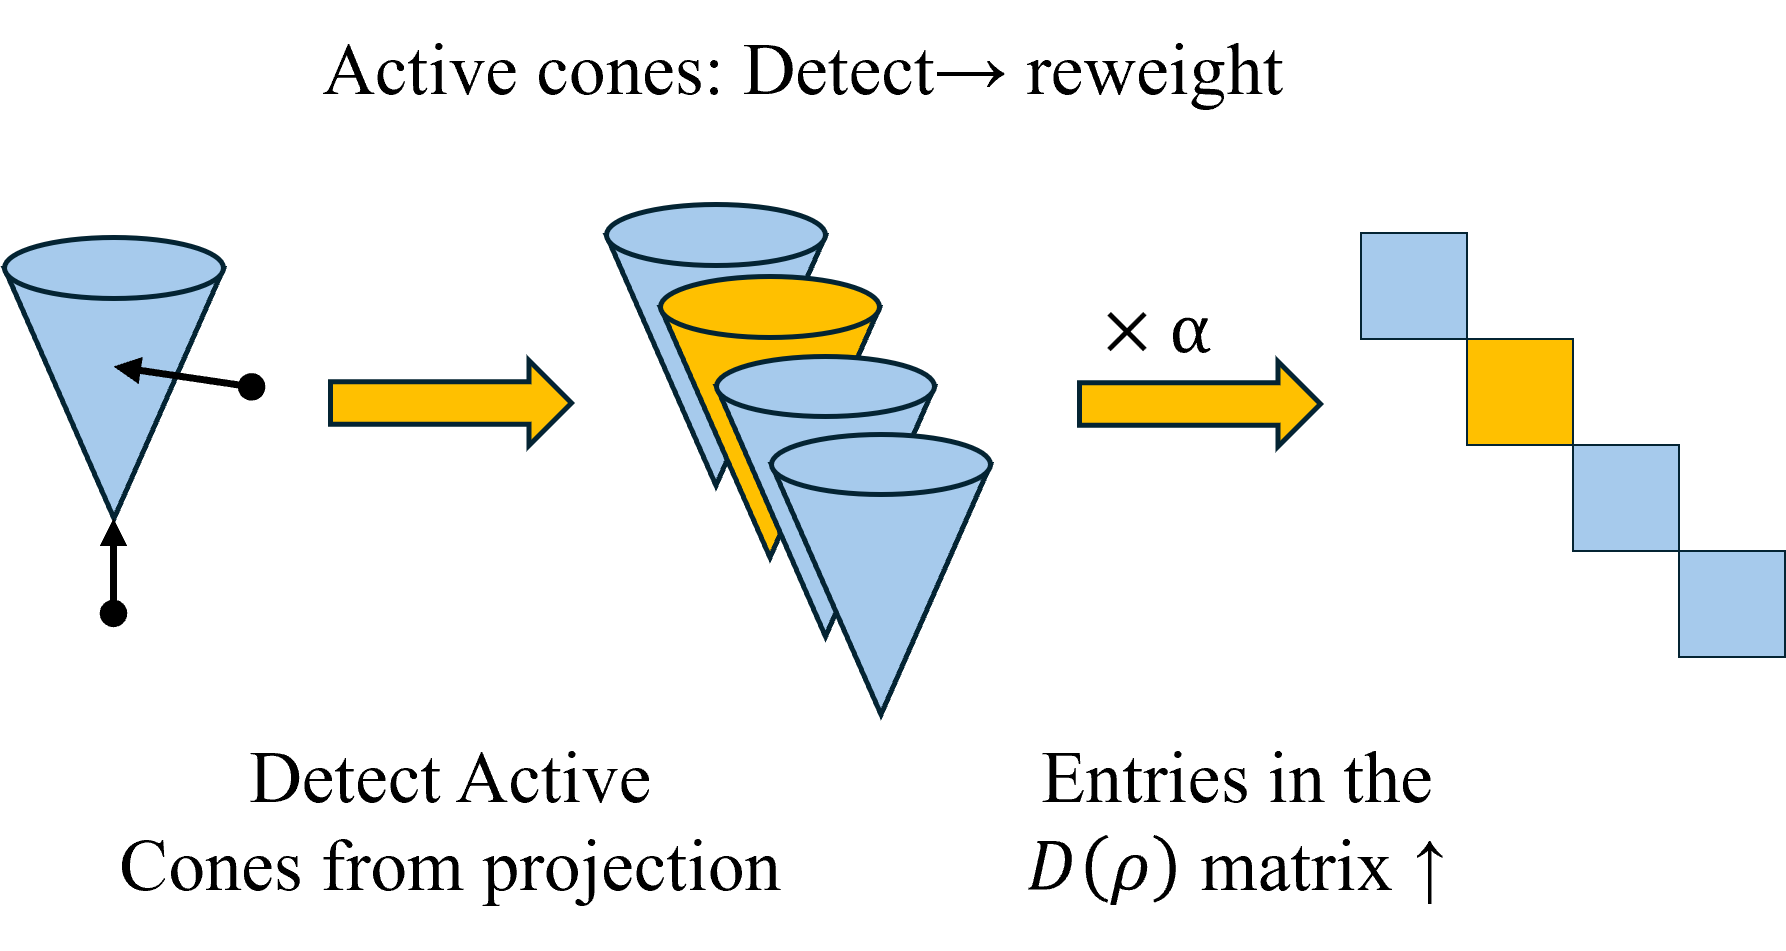
\includegraphics[width=0.70\textwidth]{figures/Res_To_Date/active_cone.png} 
\caption{Active cone identification scheme}
\label{fig:active_cone}
\end{figure}


A fixed bound $B^k$ is imposed to limit the value of the entries of $D(\rho)$ to prevent the system from becoming ill-conditioned. We denote the $j$-th entry of the  diagonal matrix $D(\rho)$ as $D(\rho)_{j,j}^k$, we clamp all entries associated with the SOC blocks to the interval:
\begin{equation}
1/B^k\leq D(\rho)_{j,j}^k\leq B^k
\label{eq:FixedBound}
\end{equation}


Since the penalty is associated with each SOC block, any update to the $D(\rho)$ matrix, must scale all diagonal entries corresponding to the same cone to maintain consistent enforcement. If the cone is active, we multiply all the associated entries by $\alpha$, otherwise do nothing. 
\begin{equation}
D(\rho)^{k+1}_{j,j} =
\begin{cases}
\alpha D(\rho)^{k}_{j,j}, &\text{if } || \boldsymbol{r}_i || \le -t_i$  or $ || \boldsymbol{r}_i || > t_i\\[2pt]
D(\rho)^{(k)}_{j,j}, & \text{otherwise},
\end{cases}
\label{eq:updateDMat}
\end{equation}


Also, at the first 200 iterations, we enforce $\alpha = 2$ when the active set is uncertain at the first 200 iterations. After the stabilization phase, we set $\alpha = 10$ for a more aggressive update. Also, we implement a simple yet effective adaptive adjustment mechanism of the value $\alpha$ near convergence, the heuristic is to reduce $\alpha$ smoothly via a quadratic rule as the iterates approach convergence, avoiding abrupt changes that could destabilize the system or perturb the final solution.

The above updates only happen if the system satisfies the following criteria:
\begin{equation}
r_{\text{dual}} \leq 0.1  \varepsilon_\mathrm{dual}
\label{eq:updateCriteria}
\end{equation} i.e., the dual feasibility condition is already well satisfied, whereas the primal residual remains far from convergence. In practice, with a reasonable initial choice of $\rho$, the dual residual typically decreases to its tolerance earlier than the primal residual.

These simple heuristics prevent the $D(\rho)$ matrix from changing drastically when approaching convergence, while preserving a robust way of updating the variables in a way that the primal and dual residuals are balanced. The idea of balancing these two residuals is inspired by the OSQP solver~\cite{OSQP}, which also adopted an adaptive $\rho$ measure, however the parameter $\rho$ updated uniformly across all constraints, whereas here we adaptively update the penalty only on the active conic blocks.

Notice that the linear constraints are unchanged during the process. Updates to the diagonal weighting matrix $D(\rho)$ modify the system matrix $A^\top D(\rho) A$. Importantly, since $D(\rho)$ only rescales constraint rows, these updates do not change the sparsity pattern of $A^\top D(\rho) A$. We therefore reuse the symbolic factorization and perform only a numerical refactorization of $A^\top D(\rho) A$ whenever $D(\rho)$ is updated, reducing the overhead of re-factorization.




\subsection{Augmented ADMM formulation}

In the GPU-accelerated 3D FELA implementation, we found that even medium-sized problems can exceed the capabilities of a relatively modest GPU (in our case, an NVIDIA RTX A1000). In practice, we observed that in 3D FELA, the condensed matrix becomes increasingly dense as the problem size grows, while the ratio of $\frac{A^\top D(\rho) A.nnz()}{A.nnz()}$ remained close to constant in 2D. This motivated us to solve the augmented linear system rather than the condensed system, with the expectation that the augmented form would lead to fewer non-zero fill-ins during factorization. In practice, we always solve the augmented linear system in 3D.

To improve the conditioning of the linear system, a regularization parameter \(\sigma\) is introduced. Although the augmented system is no longer positive definite, it remains quasi-definite and therefore admits a well-defined \(LDL^\top\) factorization~\cite{COSMO}:

\begin{equation}
\begin{bmatrix}
\sigma I & A^{T} \\
A & -D(\rho)^{-1}
\end{bmatrix}
\begin{bmatrix}
x^{k+1} \\
\upsilon
\end{bmatrix}
=
\begin{bmatrix}
-c + \sigma x^{k} \\
b - s - D(\rho)^{-1} y
\end{bmatrix}
\label{eq:AUG}
\end{equation}

 

\subsection{Alternative ellipsoidal projection scheme}

Solver performance may also be improved by adopting an alternative projection strategy. In MOSEK and in our ADMM implementation, the projection step is introduced by adding an additional set of variables \(s\) and enforcing
$Ax + s = b$,
where, for each conic constraint, \(A\) is the affine transformation matrix defined in \eqref{eq:2DSOC}. When \(\alpha = 0\), the Drucker--Prager criterion reduces to the von Mises criterion, and the corresponding SOC projection becomes equivalent to a projection onto an ellipsoid.

This ellipsoidal projection scheme was implemented only in the 3D programme. After splitting and enforcing \(x = s\), the projection step at each stress point \(i\) amounts to projecting the associated slack vector
\[
s_i^{\mathrm{trial}} = (s_{1,i}, s_{2,i}, \dots, s_{6,i})^\top
\]
onto the ellipsoid
\[
\mathcal{E} = \{\, s \in \mathbb{R}^6 \mid s^\top P s \leq 1 \,\}.
\]

The projection problem can therefore be written as
\begin{equation}
\begin{array}{ll}
\textbf{minimize}   & \dfrac{1}{2}\|s - s_i^{\mathrm{trial}}\|^2 \\[4pt]
\textbf{subject to} & s^\top P s \leq 1,
\end{array}
\label{eq:ELP}
\end{equation}
where \(s_i^{\mathrm{trial}}\) denotes the current slack vector before projection.

For stress points lying outside the ellipsoid, the inequality constraint is active at the solution, and the KKT conditions are
\begin{equation}
\begin{array}{ll}
1) & s - s_i^{\mathrm{trial}} + 2\lambda P s = 0, \\[4pt]
2) & s^\top P s = 1, \\[4pt]
3) & \lambda \geq 0.
\end{array}
\label{eq:KKT_ELP}
\end{equation}
Let
\[
\mu = 2\lambda \geq 0.
\]
Then we obtain
\begin{equation}
(I + \mu P)s = s_i^{\mathrm{trial}},
\end{equation}
and hence
\begin{equation}
s(\mu) = (I + \mu P)^{-1} s_i^{\mathrm{trial}}.
\end{equation}

We now give the formulation of the P matrix as:
\begin{equation}
P = \frac{1}{k^2}
\begin{bmatrix}
\frac{1}{3} & -\frac{1}{6} &  -\frac{1}{6} & 0 & 0 & 0 \\
-\frac{1}{6} & \frac{1}{3} &  -\frac{1}{6} & 0 & 0 & 0 \\
-\frac{1}{6} & -\frac{1}{6} & \frac{1}{3} &  0 & 0 & 0 \\
0 & 0 & 0 & 1 & 0 & 0 \\
0 & 0 & 0 & 0 & 1 & 0 \\
0 & 0 & 0 & 0 & 0 & 1 
\end{bmatrix}
\end{equation}
Substituting \(s(\mu)\) into the active constraint yields the scalar root-finding problem
\begin{equation}
\phi(\mu) = s(\mu)^\top P s(\mu) - 1 = 0,
\end{equation}
which can be solved efficiently by Newton's method:
\begin{equation}
\mu_{j+1} = \mu_j - \frac{\phi(\mu_j)}{\phi'(\mu_j)}.
\label{eq:Newt}
\end{equation}

In practice, although a large number of stress points must be projected, the high-level parallelisation provided by a customised CUDA kernel reduces the cost of this step to only about \(3\%\) of the total solution time.

\subsection{Implementation of the solver on CUDA}

Profiling of the code on CPU showed that apart from the obvious bottleneck of the solve operation that took place in every iteration, the various sparse matrix manipulations, if not handled efficiently, may also significantly degrade overall solver performance. To address this, the implementation makes intensive use of GPU acceleration, and the following improvements were made:

\paragraph{cuDSS for solving the linear system}



In the condensed formulation, the KKT system is symmetric positive-definite. As a result, cuDSS internally uses a Cholesky factorization path, which is faster and more memory-efficient than the general-purpose $LDL^\top$ decomposition. This choice leads to significant runtime improvements in the solve phase of each ADMM iteration in 2D FELA, however, in 3D, when memory usage of a condensed formulation exceeds the capacity of the GPU, the augmented formulation, even though it used a sparse $LDL^\top$ decomposition, was faster in time per-iteration.

\paragraph{cuBLAS and cuSPARSE for efficient construction of vectors}

cuBLAS is a CUDA implementation of BLAS, which enables convenient access to GPU-accelerated BLAS operations. cuSPARSE is a CUDA library that contains many commonly used matrix manipulation subroutines. 

\paragraph{CUDA kernel functions for customized variable updates}

CUDA kernel functions are special C functions executed on the GPU in a highly parallelised fashion~\cite{GPU_ADMM}. Each thread runs the same instructions on different data, making them inherently suitable for SIMD-style computations. While many standard linear algebra operations are efficiently handled by highly optimized libraries such as cuBLAS and cuSPARSE, several complex or non-standard operations required in our solver are not directly supported. 

For example, the non-uniform scaling of the variables and matrices, and simultaneous projection onto $N_{SOC}$ second-order cones, and parallel updates of intermediate vectors fall outside of the scope of existing CUDA libraries. 

\paragraph{All operations completed on GPU}

Though the construction of the KKT matrix and warm-starting is completed outside of the GPU, all the subsequent ADMM iterations are completed on the GPU, only passing the primal and dual residual and the current objective back to the CPU. This design significantly eliminated the overhead introduced by the frequent GPU-CPU data transfers.

\section{Numerical Experiments}

In this section, we present 3 sets of classical FELA benchmark problems to assess the performance of the proposed ADMM solver in comparison with two state-of-the-art commercial interior-point solvers, MOSEK and Gurobi.

In each of the following examples, we first describe the problem setup and then present numerical results to assess the accuracy, robustness, and scalability of the proposed ADMM solver in comparison with IPM codes. For both the 2D plane-strain and 3D cases, three benchmark problems are considered: the rigid platen, strip footing, and vertical cut problems. For each benchmark, the computational performance of the proposed ADMM solver is compared with that of commercial interior-point solvers in terms of solution time and accuracy. Adaptive mesh refinement results are also presented to demonstrate the FELA formulation’s ability to capture localized failure mechanisms efficiently. 

\subsection{Experimental setup}

Linear stress elements were used in the comparison of accuracy and speed of the in-house solver and IPM solvers in all three geotechnical problems. We use a structured mesh as test problems to the solvers in the benchmark comparison part, and use an adaptively refined mesh to give better quality solution and to demonstrate the failure pattern.

All CPU code was run on an Intel Core i7-12700H, and all GPU code were run on a NVIDIA RTX A1000. We assume Tresca soil with $c = 1$ on 2D problems, and von Mises soil with $k = 1$ on 3D problems. The GPU implementation was developed using NVIDIA CUDA~12.8 and cuDSS~0.5.0. Its performance was compared with MOSEK~11.0 and Gurobi~12.0.2, which served as the commercial interior-point method baselines. In all experiments, MOSEK and Gurobi were run using their default termination criteria on 14 CPU cores.
%%
%\[
%\mathrm{pfeas} \le \varepsilon_{\mathrm{pfeas}}, 
%\qquad 
%\mathrm{dfeas} \le \varepsilon_{\mathrm{dfeas}},
%\]
%with
%\[
%\varepsilon_{\mathrm{pfeas}} = \varepsilon_{\mathrm{dfeas}} = 10^{-3}.
%\]
%%

\subsection{2D Plane Strain Benchmark Problems}

\subsubsection {Rigid Platen Problem}
\paragraph{Problem setup} In this problem, a block of Tresca soil of size $L\times0.5L$ is subjected to compression between two rigid platens. The interfaces between the platens and the soil are assumed to be fully rough. Symmetric boundary conditions are applied to the left and bottom boundaries, while the right boundary is left free. An illustrative representation of the physical setup is provided in Figure~\ref{fig:2PR_CS}.

The exact solution of the load multiplier for the rigid platen problem considered here, $\beta = 2.42768$, was first given by Salençon~\cite{ daSilva_2020, Salencon}. 



\begin{figure}[htbp]
  \centering
  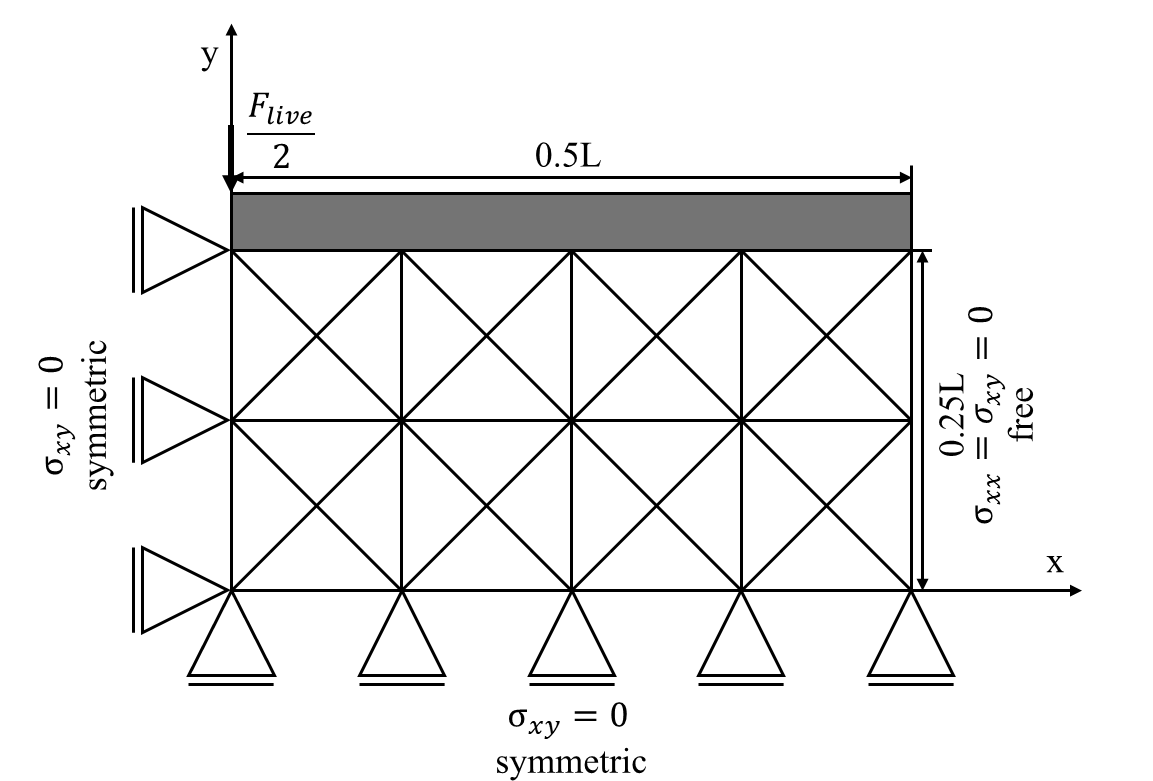
\includegraphics[width=0.50\textwidth]{figures/Res_To_Date/2PR_config.png}
  \hfill
  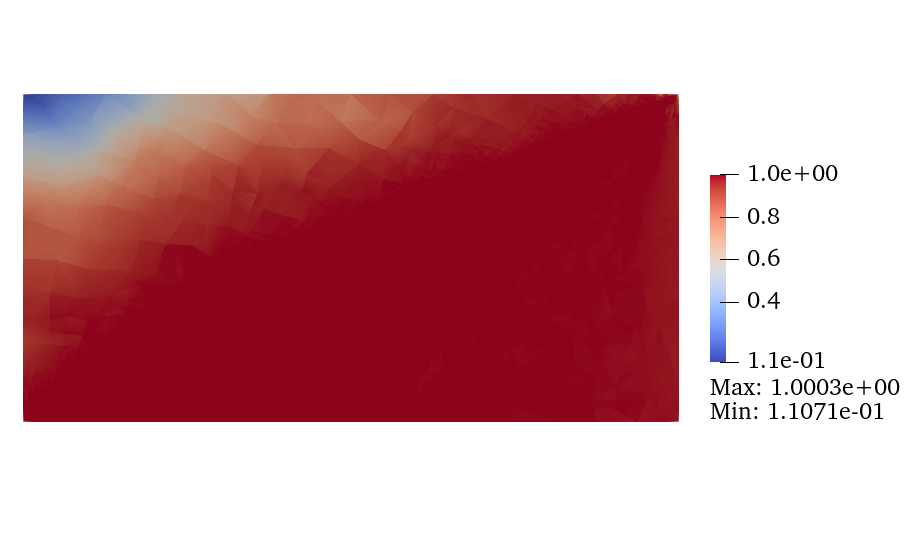
\includegraphics[width=0.46\textwidth]{figures/Res_To_Date/2PR_solution.png}
  \caption{Rigid platen problem. \textbf{Left}: physical configuration; \textbf{Right}: obtained yield function field using AMR with linear stress elements}
  \label{fig:2PR_CS}
\end{figure}

\paragraph{Benchmark comparison using sturctured mesh} 

The proposed ADMM solver is benchmarked against the commercial interior-point solvers MOSEK and Gurobi using structured meshes of linear stress elements with progressively refined discretizations.


\begin{table}[htbp]
\centering
\caption{Solver performance comparison on the 2D rigid platen benchmark for different mesh discretizations}
\label{tab:2PR_timecomp}

\begin{tabular}{@{}C{1.7cm}C{1.7cm}C{1.5cm}C{2.0cm}C{2.3cm}C{2.3cm}C{2.3cm}@{}}
\toprule
\multicolumn{2}{c}{\textbf{Problem size}} &
\textbf{Solver} &
\textbf{Solve time (s)} &
\textbf{Collapse multiplier} &
\textbf{Iterations}&
\textbf{Time-per-iter (s)}
\tabularnewline
\cmidrule(lr){1-2}
\textbf{$N_{\mathrm{elem}}(\times 10^3)$} &
\textbf{$N_{\mathrm{var}}(\times 10^6)$} &
&
&
&
\tabularnewline
\midrule

\multirow{3}{*}{20.0}
& \multirow{3}{*}{0.18}
& MOSEK  & 8.80 & 2.42465 &  32  &0.37 \tabularnewline
& & Gurobi & 6.96   & 2.42465&   26    & 0.28 \tabularnewline
& & ADMM   & 2.66 & 2.42467&  340  & 0.0078 \tabularnewline

\addlinespace

\multirow{3}{*}{28.8}
& \multirow{3}{*}{0.26}
& MOSEK  & 31.75 & 2.42514 &  35  &0.91 \tabularnewline
& & Gurobi & 13.98    & 2.42514 & 30  & 0.68 \tabularnewline
& & ADMM   & 3.62  & 2.42516& 260 & 0.014 \tabularnewline

\addlinespace

\multirow{3}{*}{51.2}
& \multirow{3}{*}{0.46}
& MOSEK  & 60.03 & 2.42576 & 46 & 1.11 \tabularnewline
& & Gurobi & 27.60    & 2.42577 & 34 & 1.31 \tabularnewline
& & ADMM   & 5.74  & 2.42577& 300 & 0.019 \tabularnewline

\addlinespace

\multirow{3}{*}{80.0}
& \multirow{3}{*}{0.72}
& MOSEK  & 43.14 & 2.42614 & 38 & 1.14 \tabularnewline
& & Gurobi & 50.81    & 2.42614   & 27   & 2.48 \tabularnewline
& & ADMM   & 9.82  & 2.42611 & 340 & 0.029 \tabularnewline

\addlinespace

\multirow{3}{*}{204.8}
& \multirow{3}{*}{1.84}
& MOSEK  & 95.24 & 2.42669 & 39 & 3.024 \tabularnewline
& & Gurobi & 342.17    & 2.42671  &  32  & 12.01 \tabularnewline
& & ADMM   & 20.36 & 2.42669&  280  & 0.073 \tabularnewline

\bottomrule
\end{tabular}

\vspace{0.5em}
\end{table}

Table~\ref{tab:2PR_timecomp} shows that the proposed solver delivers superior computational performance, achieving a speedup of \(4\times\) to \(10\times\) over the state-of-the-art IPM solvers, while maintaining high solution accuracy in all cases. For each mesh discretization, all three solvers converge to closely comparable collapse multipliers. The problem sizes are reported in Table~\ref{tab:2PR_timecomp}, ranging from 0.18 million variables to 1.84 million variables. 


The computed collapse multipliers remain below the analytical solution reported by Salen\c{c}on~\cite{daSilva_2020, Salencon}. This gap is primarily due to the use of a structured mesh. Using higher-order stress elements may mitigate this effect and yield a tighter lower bound. We nonetheless adopt structured meshes in this example to ensure controlled and consistent problem generation, which is desirable for a fair performance comparison. Overall, the results reported here demonstrated that the proposed ADMM methodology works well on these types of PDE-constrained optimization problem.


\paragraph{Adaptive mesh refinement solution}

Using AMR, we obtain a tighter lower bound solution of $\beta = 2.426787$ using linear stress elements, together with AMR, the resulting yield function is shown in Figure~\ref{fig:2PR_CS}, with the final adaptively refined mesh after 10 refinements shown in Figure~\ref{fig:2PR_mesh}. This gives a relative error of only 0.036\%, the refined mesh concentrated around the yielded area. Moreover, the zone that had been refined the most agrees well with the solutions of da Silva~\cite{daSilva_2020} and with the classical slip line solutions~\cite{Slip_Line_Hosford}.

\begin{figure}
\centering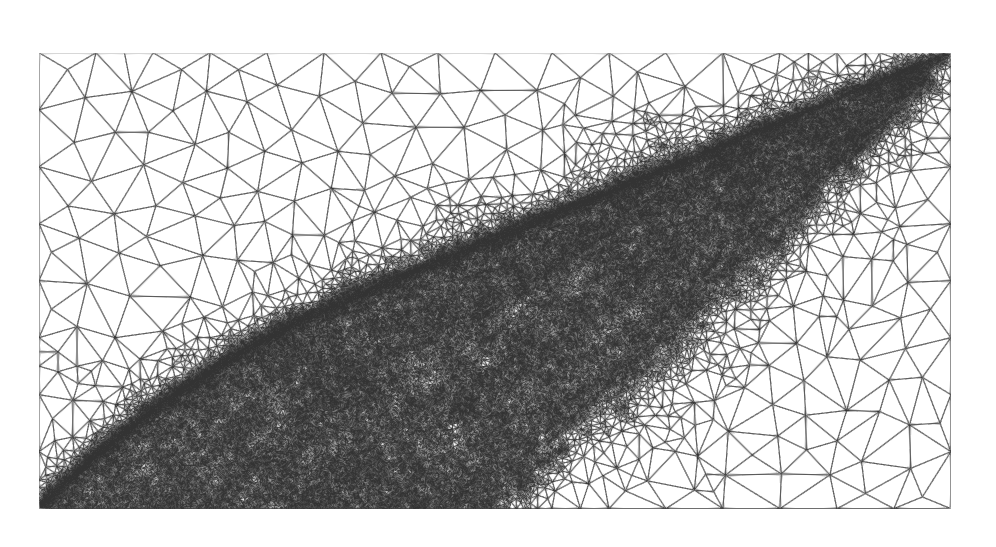
\includegraphics[width=0.8\textwidth]{figures/Res_To_Date/2PR_mesh.png} 
\caption[AMR result of the rigid platen problem]{AMR result of the rigid platen problem}
\label{fig:2PR_mesh}
\end{figure}



\subsubsection{Strip Footing Problem}
\paragraph{Problem setup}
An illustrative representation of the problem is shown in Figure~\ref{fig:SF_CS}. Here, a rigid body is placed at the upper-left corner of the domain to represent a strip footing. A fixed boundary condition is applied on the right and bottom edges, and a symmetric boundary condition on the left edge. The fixed boundaries are sufficiently far from the footing to have a minimal effect  on the result.


The ultimate bearing capacity of a strip footing on weightless cohesive soil is a foundational result in geotechnical engineering. The exact solution of the load multiplier to this problem is $\beta = 2+\pi$, a result first derived by Prandtl~\cite{ Sloan_stability_analysis, 2DLB, Prandtl}. Martin developed software ABC for calculating the ultimate bearing capacity of this footing using the method of characteristics~\cite{Slip_Line_2005}. A FELA-based solution to this problem with adaptive mesh refinement was first given by Lyamin~\cite{adaptive_mesh_Lyamin}, demonstrating that the approach can deliver accurate collapse loads while systematically assessing a range of adaptive remeshing strategies.


\begin{figure}[htbp]
  \centering
  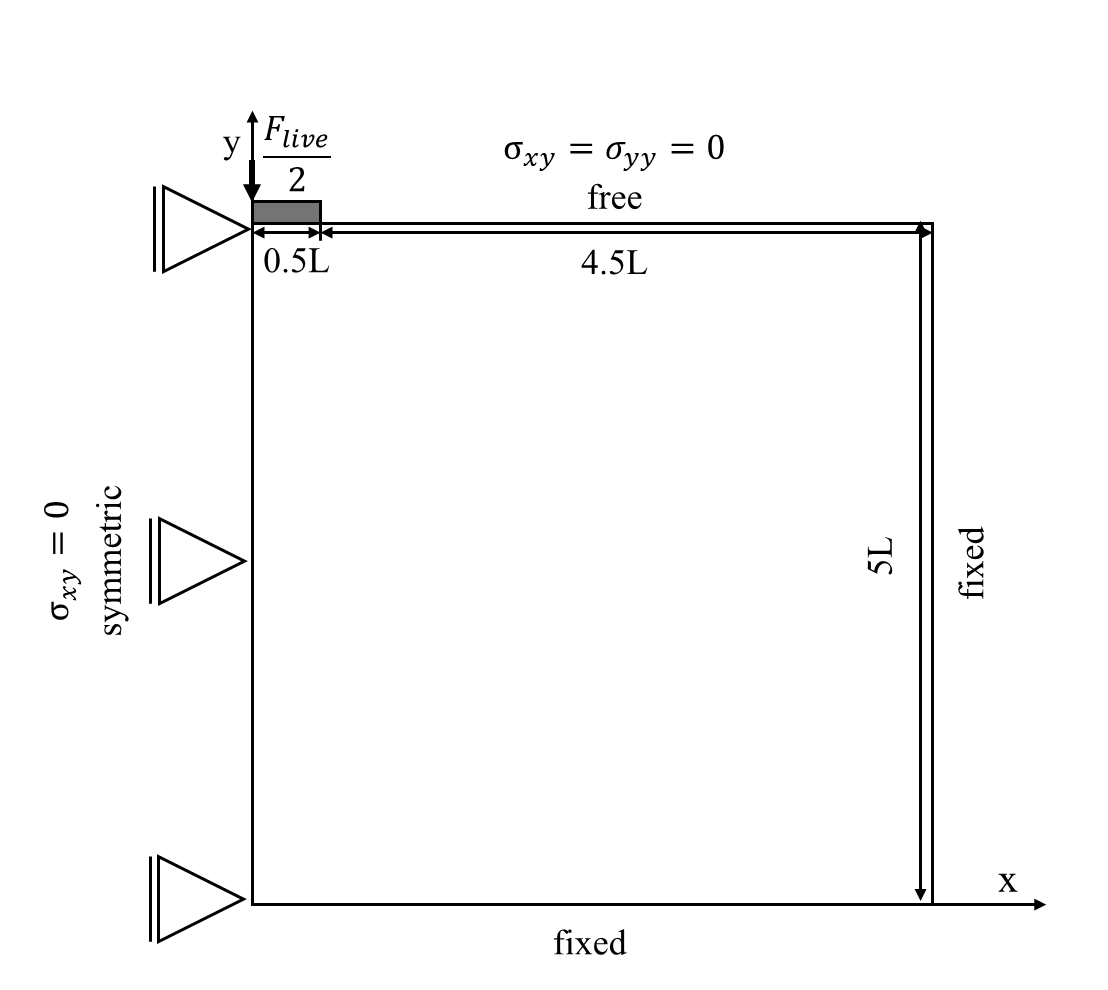
\includegraphics[width=0.50\textwidth]{figures/Res_To_Date/SF_config.png}
  \hfill
  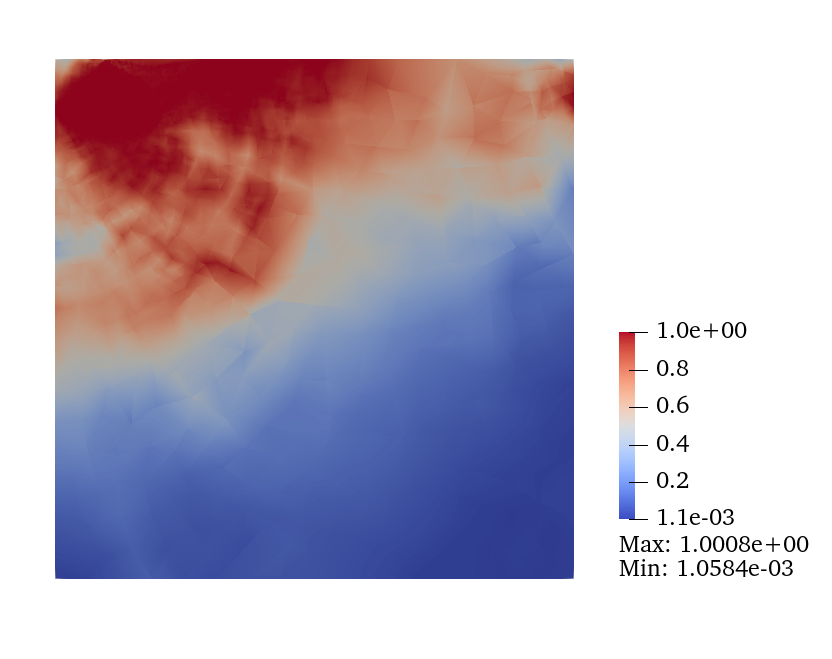
\includegraphics[width=0.47\textwidth]{figures/Res_To_Date/SF_solution.png}
  \caption{Strip footing problem. \textbf{Left}: physical configuration; \textbf{Right}: solution of the yield function using AMR and linear stress elements}
  \label{fig:SF_CS}
\end{figure}

\paragraph{Benchmark comparison using structured mesh} We first demonstrate the performance of our 2D condensed-form ADMM solver on different mesh discretizations, all using linear stress elements. 



\begin{table}[htbp]
\centering
\caption{Solver performance comparison on the 2D strip footing benchmark for different mesh discretization}
\label{tab:SF_detail}

\begin{tabular}{@{}C{1.7cm}C{1.7cm}C{1.5cm}C{2.0cm}C{2.3cm}C{2.3cm}C{2.3cm}@{}}
\toprule
\multicolumn{2}{c}{\textbf{Problem size}} &
\textbf{Solver} &
\textbf{Solve time (s)} &
\textbf{Collapse multiplier} &
\textbf{Iterations}&
\textbf{Time-per-iter (s)}
\tabularnewline
\cmidrule(lr){1-2}
\textbf{$N_{\mathrm{elem}}(\times 10^3)$} &
\textbf{$N_{\mathrm{var}}(\times 10^6)$} &
&
&
&
\tabularnewline
\midrule

\multirow{3}{*}{40.0}
& \multirow{3}{*}{0.36}
& MOSEK  & 27.37 & 5.09752 &  32  &0.86 \tabularnewline
& & Gurobi & 24.73   & 5.09753&   231    & 1.09 \tabularnewline
& & ADMM   & 6.08 & 5.09768&  440  & 0.014 \tabularnewline

\addlinespace

\multirow{3}{*}{57.6}
& \multirow{3}{*}{0.52}
& MOSEK  & 48.59 & 5.10470 &  38  & 1.28 \tabularnewline
& & Gurobi & 26.78    & 5.10470 & 27  & 1.26 \tabularnewline
& & ADMM   & 8.47  & 5.10482& 440 & 0.019 \tabularnewline

\addlinespace

\multirow{3}{*}{102.4}
& \multirow{3}{*}{0.92}
& MOSEK  & 204.05 & 5.11383 & 50 & 5.57 \tabularnewline
& & Gurobi & 173.61    & 5.11383 & 35 & 4.08 \tabularnewline
& & ADMM   & 13.77  & 5.11392 & 400 & 0.034 \tabularnewline

\addlinespace

\multirow{3}{*}{160.0}
& \multirow{3}{*}{1.44}
& MOSEK  & 126.85 & 5.11932 & 33 & 3.84 \tabularnewline
& & Gurobi & 270.60    & 5.11932   & 35   & 8.59 \tabularnewline
& & ADMM   & 25.82  & 5.11939 & 460 & 0.056 \tabularnewline

\bottomrule
\end{tabular}

\vspace{0.5em}
\end{table}

Table~\ref{tab:SF_detail} shows that the proposed GPU-based ADMM solver remains faster than the CPU-parallelized IPM solver MOSEK and Gurobi, while producing almost identical collapse multipliers. The observed speedup ranges from $3.12\times$ to $5.7\times$ for MOSEK, and $6.04\times$ to $17.28\times$ for Gurobi. Although this improvement is less pronounced than that obtained for the 2D rigid platen problem, it still demonstrates the efficiency of the proposed solver on classical FELA problems.

The final load multiplier remains below Prandtl's analytical solution of $2+\pi$, with an error of only $0.27\%$. This discrepancy is mainly due to the use of linear stress elements on structured meshes for benchmarking. A tighter LB solution is obtained below using AMR and linear stress elements:

\paragraph{Adaptive mesh refinement solution} Here we demonstrate an ADMM–FELA framework enhanced by AMR using linear stress elements. By mapping the solution from the previous mesh onto the refined mesh as the initial iterate, we achieve a substantial reduction in iterations while maintaining accuracy. The final yield function field, after 9 refinements, is given in Figure~\ref{fig:SF_CS}. Solving this problem yields a load multiplier of $\beta = 5.13648$, while only using 58.5 seconds in its final iteration. The obtained load multiplier agrees well with the analytical solution by Prandtl~\cite{Prandtl, 2DLB}.

\begin{figure}[htbp]
  \centering
  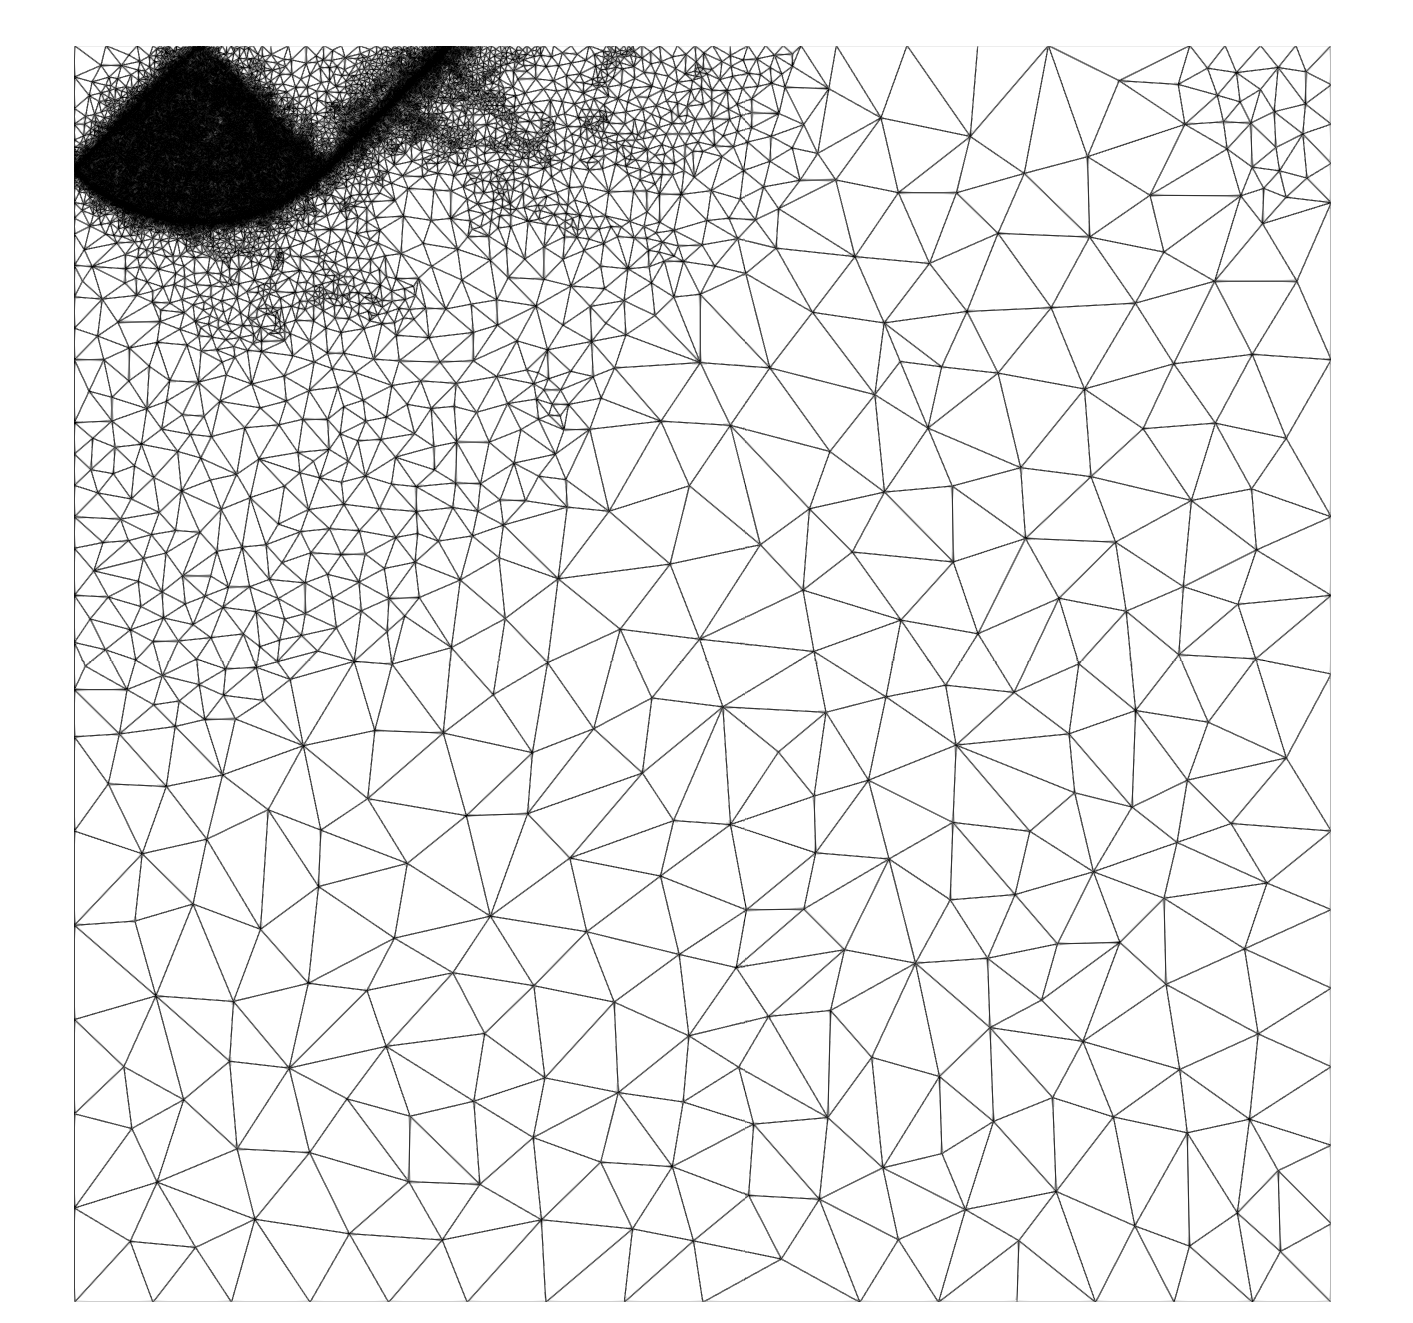
\includegraphics[width=0.37\textwidth]{figures/Res_To_Date/SF_mesh.png}
  \hfill
  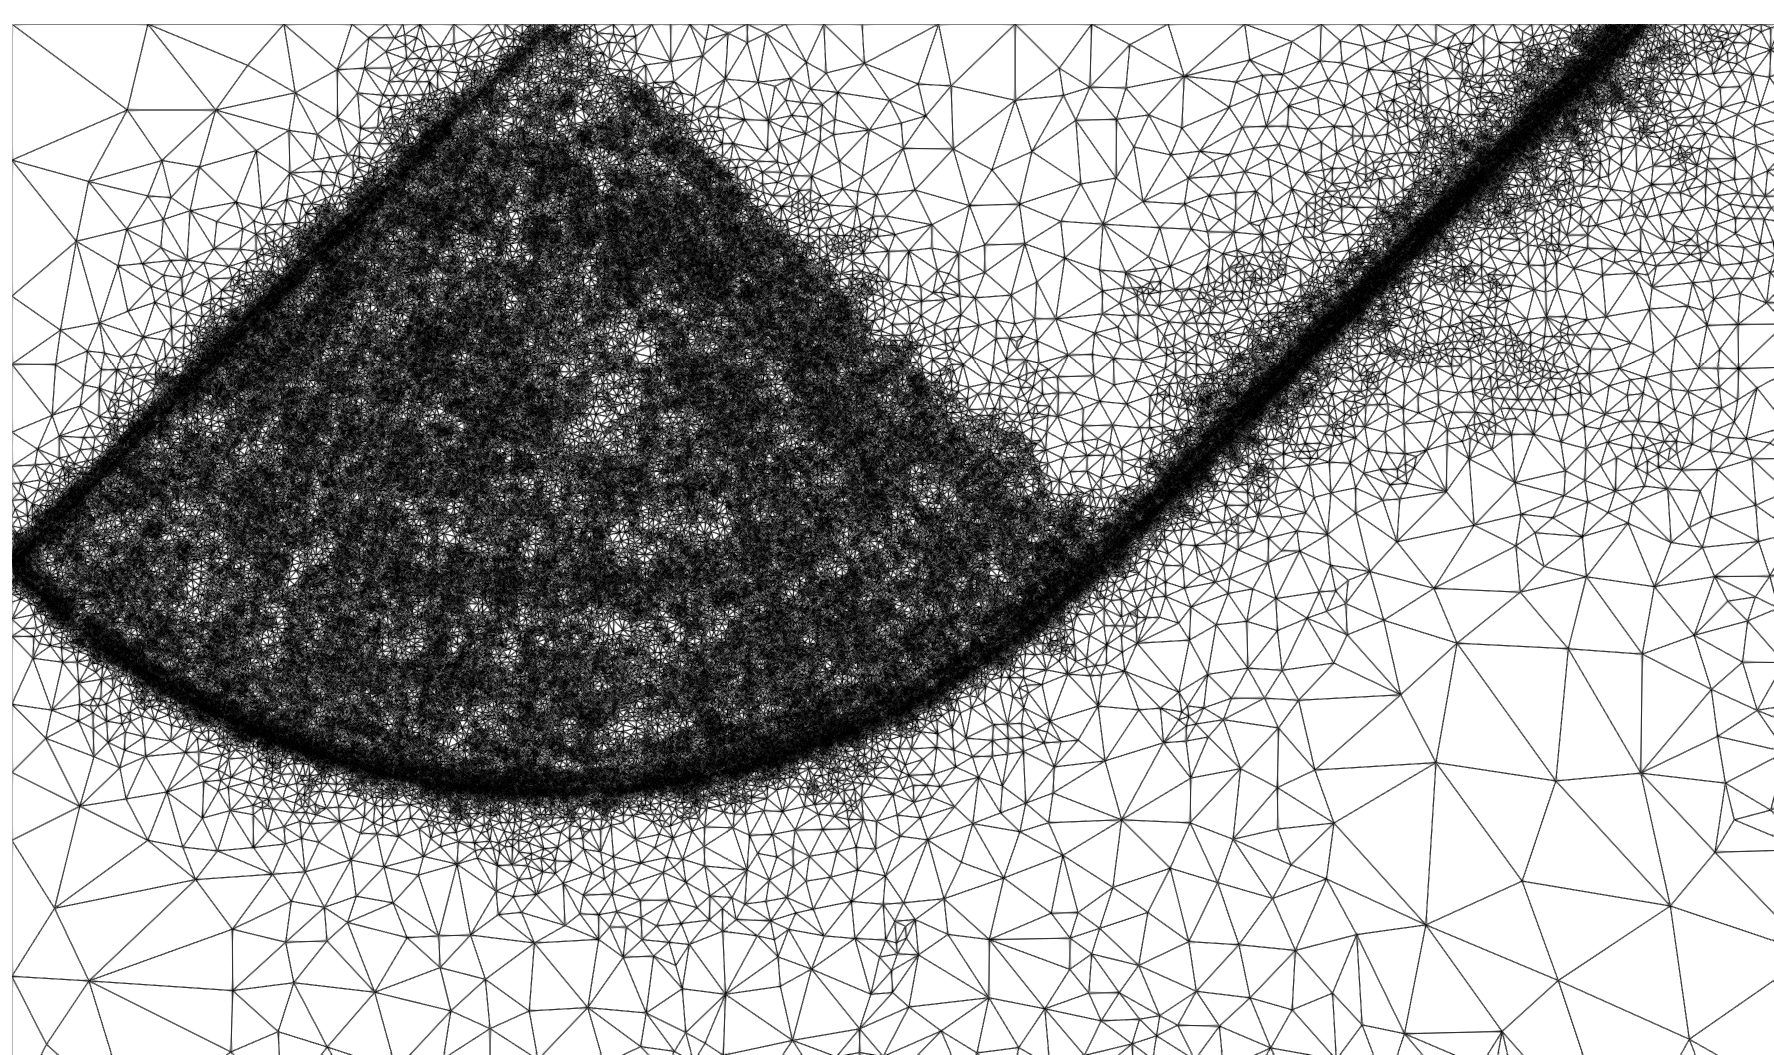
\includegraphics[width=0.59\textwidth]{figures/Res_To_Date/SF_mesh_slip_line.png}
  \caption{AMR mesh of the strip footing problem in plane strain. \textbf{Left}: overall obtained mesh; \textbf{Right}: zoomed view highlighting the refined area}
  \label{fig:SF_Mesh}
\end{figure}
The resulting AMR mesh shown in Figure~\ref{fig:SF_Mesh} is consistent with the sequential limit-analysis meshes reported by Kong~\cite{Kong_2017} and Martin~\cite{Slip_Line_2005, Martin_2011}, in that the refined region correctly matches the slip-line zone. 

This example also highlights the overall efficiency of the proposed solver, which attains rapid convergence on large-scale problems. Our solver converges easier due to exploiting the problem structure by warm-starting each AMR solve with the solution from the previous mesh.


\subsubsection{Vertical Cut Problem}


\paragraph{Problem setup}
We consider a square soil block with a vertical excavation on its left side, subjected to a uniform body force representing a live load. The top surface and the excavated left boundary are assumed to be free, while the right and bottom boundaries are taken as rough and fixed. An illustrative representation of the problem and a numerical solution given by using AMR is shown in Figure~\ref{fig:VC_CS}. This benchmark is of particular interest because the uniform body force introduces a dense column into the matrix $A$, which can pose a challenge for solver performance.

Although, to the best of the authors' knowledge, no analytical solution has been reported in the literature, Martin~\cite{Martin_2011} provided a tight bound on the ultimate bearing capacity, $3.7764904 < N < 3.7764911$, using finite element limit analysis with adaptive mesh refinement. The corresponding slip-line field was also obtained using this approach.

\begin{figure}[htbp]
  \centering
  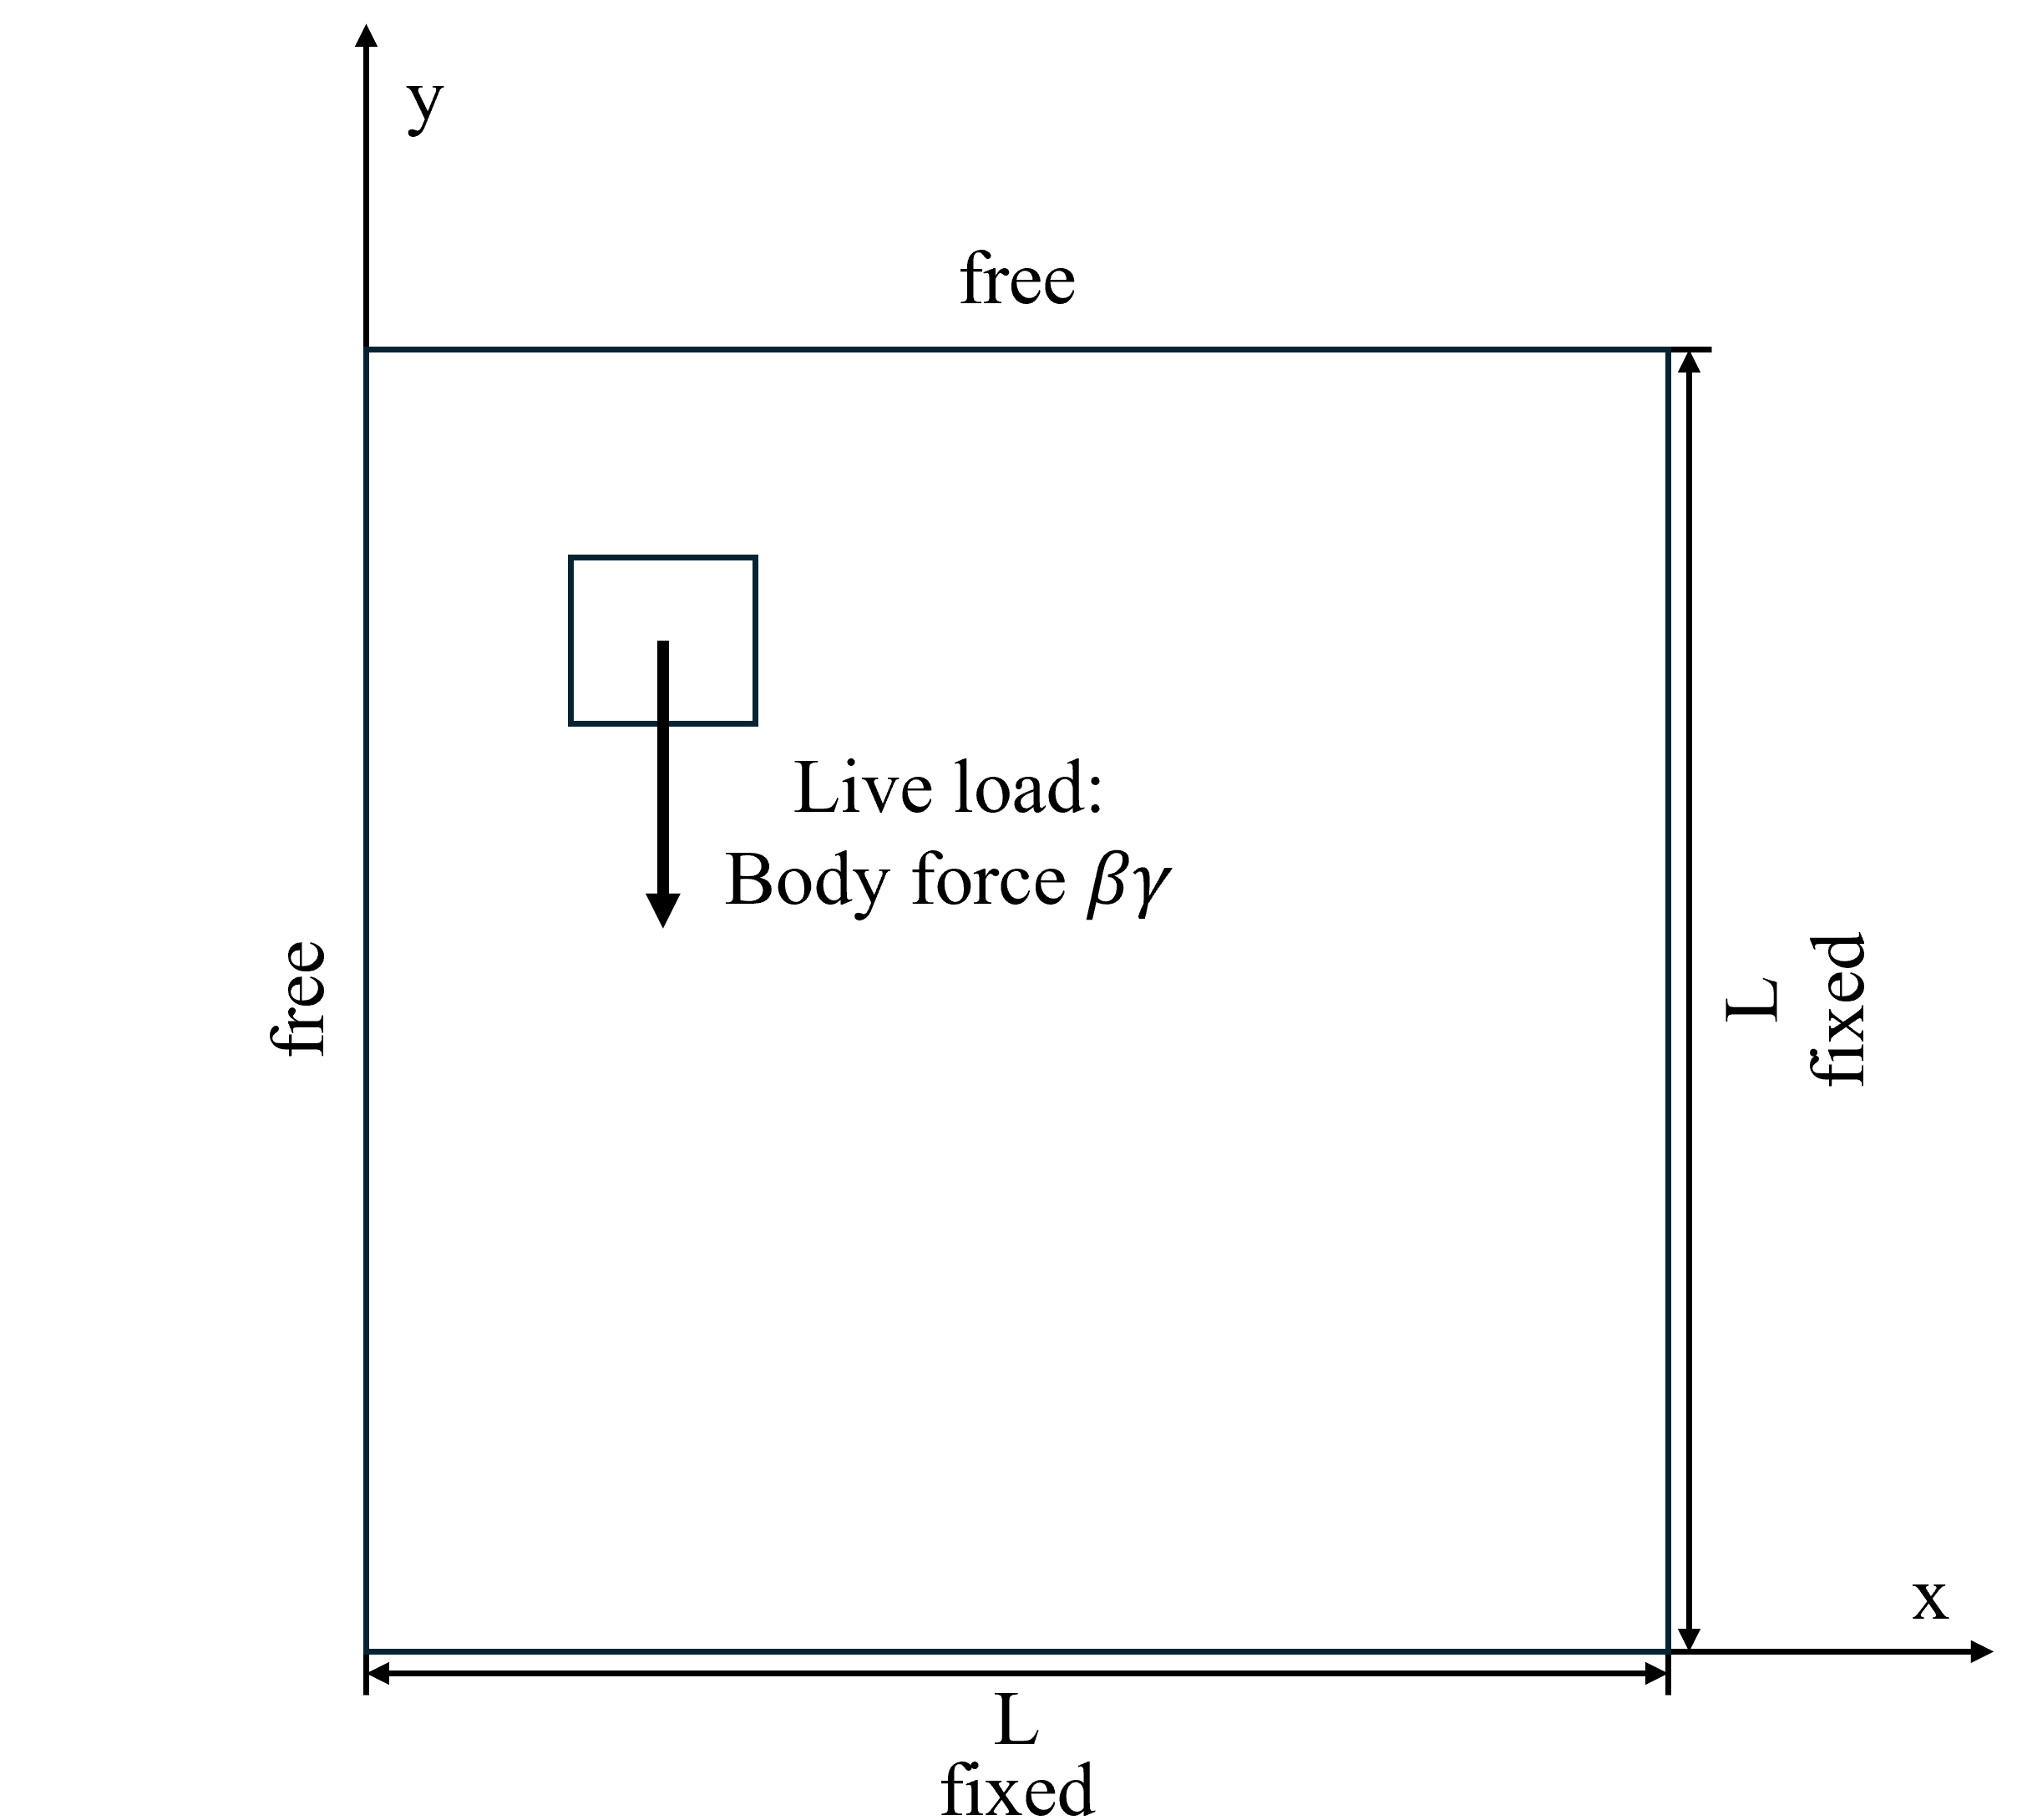
\includegraphics[width=0.48\textwidth]{figures/Res_To_Date/VC_config.png}
  \hfill
  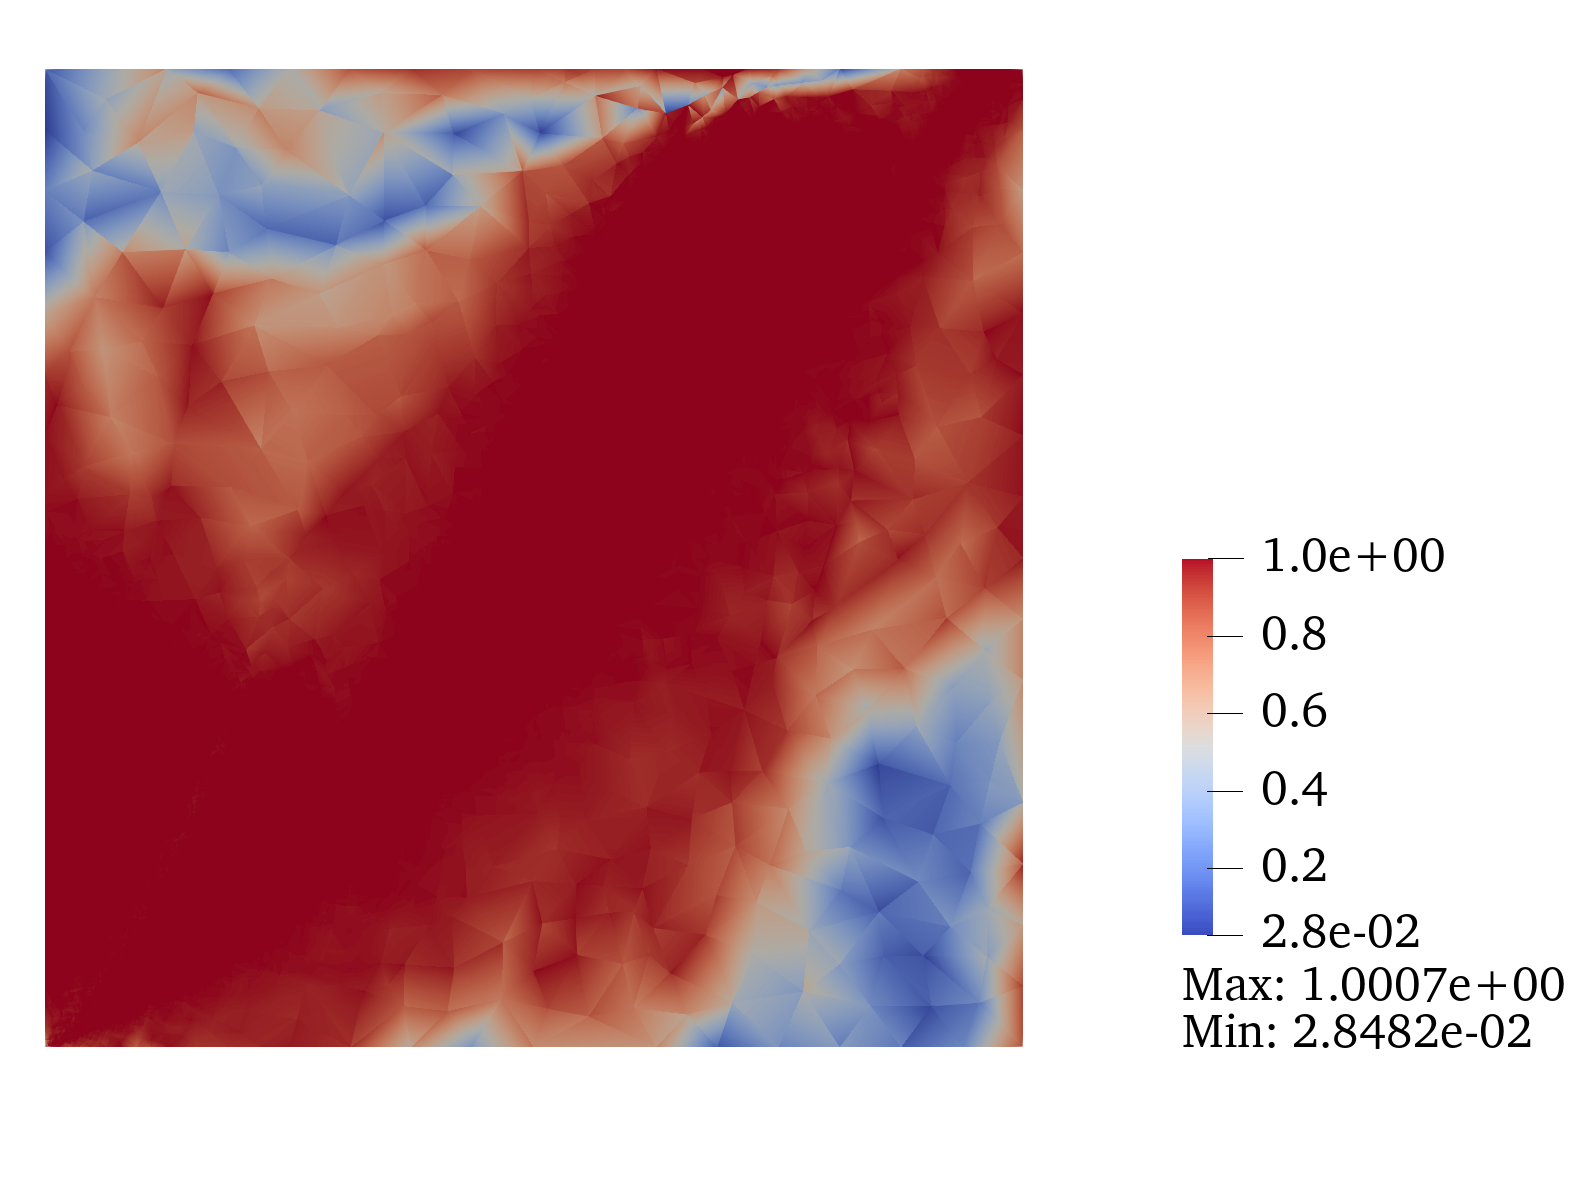
\includegraphics[width=0.48\textwidth]{figures/Res_To_Date/VCSM_SOL.png}
  \caption{Vertical cut problem. \textbf{Left}: physical configuration; \textbf{Right}: obtained yield function field}
  \label{fig:VC_CS}
\end{figure}



\paragraph{Benchmark Comparison using structured mesh}
We first assess the performance of the proposed ADMM solver using a sequence of increasingly refined meshes using linear stress elements. 

As shown in Table~\ref{tab:VC_timecomp}, the proposed ADMM solver constantly outperforms the IPM solvers in problems with dimension ranging from 0.36 to 1.44 million variables. ADMM attained a speedup from 6.6$\times$ to 17.6$\times$ compared with MOSEK, and from 6.0$\times$ to 17.3$\times$ with Gurobi. Even with the improvements made to speed up convergence, the problems still takes around 300 to 500 iterations, but each iteration is considerably cheaper than the IPM iterations. Also, the ADMM solver attained the speedup while preserving accuracy, obtaining a nearly identical load multiplier with the accurate IPM solvers.

\begin{table}[htbp]
\centering
\caption{Solver performance comparison on the 2D vertical cut benchmark for different mesh discretization}
\label{tab:VC_timecomp}

\begin{tabular}{@{}C{1.7cm}C{1.7cm}C{1.5cm}C{2.0cm}C{2.3cm}C{2.3cm}C{2.3cm}@{}}
\toprule
\multicolumn{2}{c}{\textbf{Problem size}} &
\textbf{Solver} &
\textbf{Solve time (s)} &
\textbf{Collapse multiplier} &
\textbf{Iterations}&
\textbf{Time-per-iter (s)}
\tabularnewline
\cmidrule(lr){1-2}
\textbf{$N_{\mathrm{elem}}(\times 10^3)$} &
\textbf{$N_{\mathrm{var}}(\times 10^6)$} &
&
&
&
\tabularnewline
\midrule

\multirow{3}{*}{40.0}
& \multirow{3}{*}{0.36}
& MOSEK  & 42.90 & 3.77269 &  40  &1.12 \tabularnewline
& & Gurobi & 39.27   & 3.77269&   34    & 1.28 \tabularnewline
& & ADMM   & 4.14 & 3.77255&  460  & 0.025 \tabularnewline

\addlinespace

\multirow{3}{*}{57.6}
& \multirow{3}{*}{0.52}
& MOSEK  & 43.08 & 3.77334 &  46  & 1.09 \tabularnewline
& & Gurobi & 57.85    & 3.77333 & 37  & 1.77 \tabularnewline
& & ADMM   & 5.47  & 3.77330 & 340 & 0.035\tabularnewline

\addlinespace

\multirow{3}{*}{102.4}
& \multirow{3}{*}{0.92}
& MOSEK  & 116.40 & 3.77412 & 43 & 3.13 \tabularnewline
& & Gurobi & 164.12    & 3.77413 & 43 & 4.13 \tabularnewline
& & ADMM   & 11.66  & 3.77410 & 320 & 0.071 \tabularnewline

\addlinespace

\multirow{3}{*}{160.0}
& \multirow{3}{*}{1.44}
& MOSEK  & 303.89 & 3.77459 & 50 & 6.66 \tabularnewline
& & Gurobi &  298.47   & 3.77460   & 45   & 7.14 \tabularnewline
& & ADMM   & 17.27  & 3.77458 & 300 & 0.13 \tabularnewline

\bottomrule
\end{tabular}

\vspace{0.5em}
\end{table}



\paragraph{Adaptive Mesh Solution}
With the use of AMR, the best LB estimation we may obtain is 3.775063 using linear stress elements, the adaptive refined mesh is shown in Figure~\ref{fig:VC_AMR}. 

\begin{figure}[htbp]
  \centering
  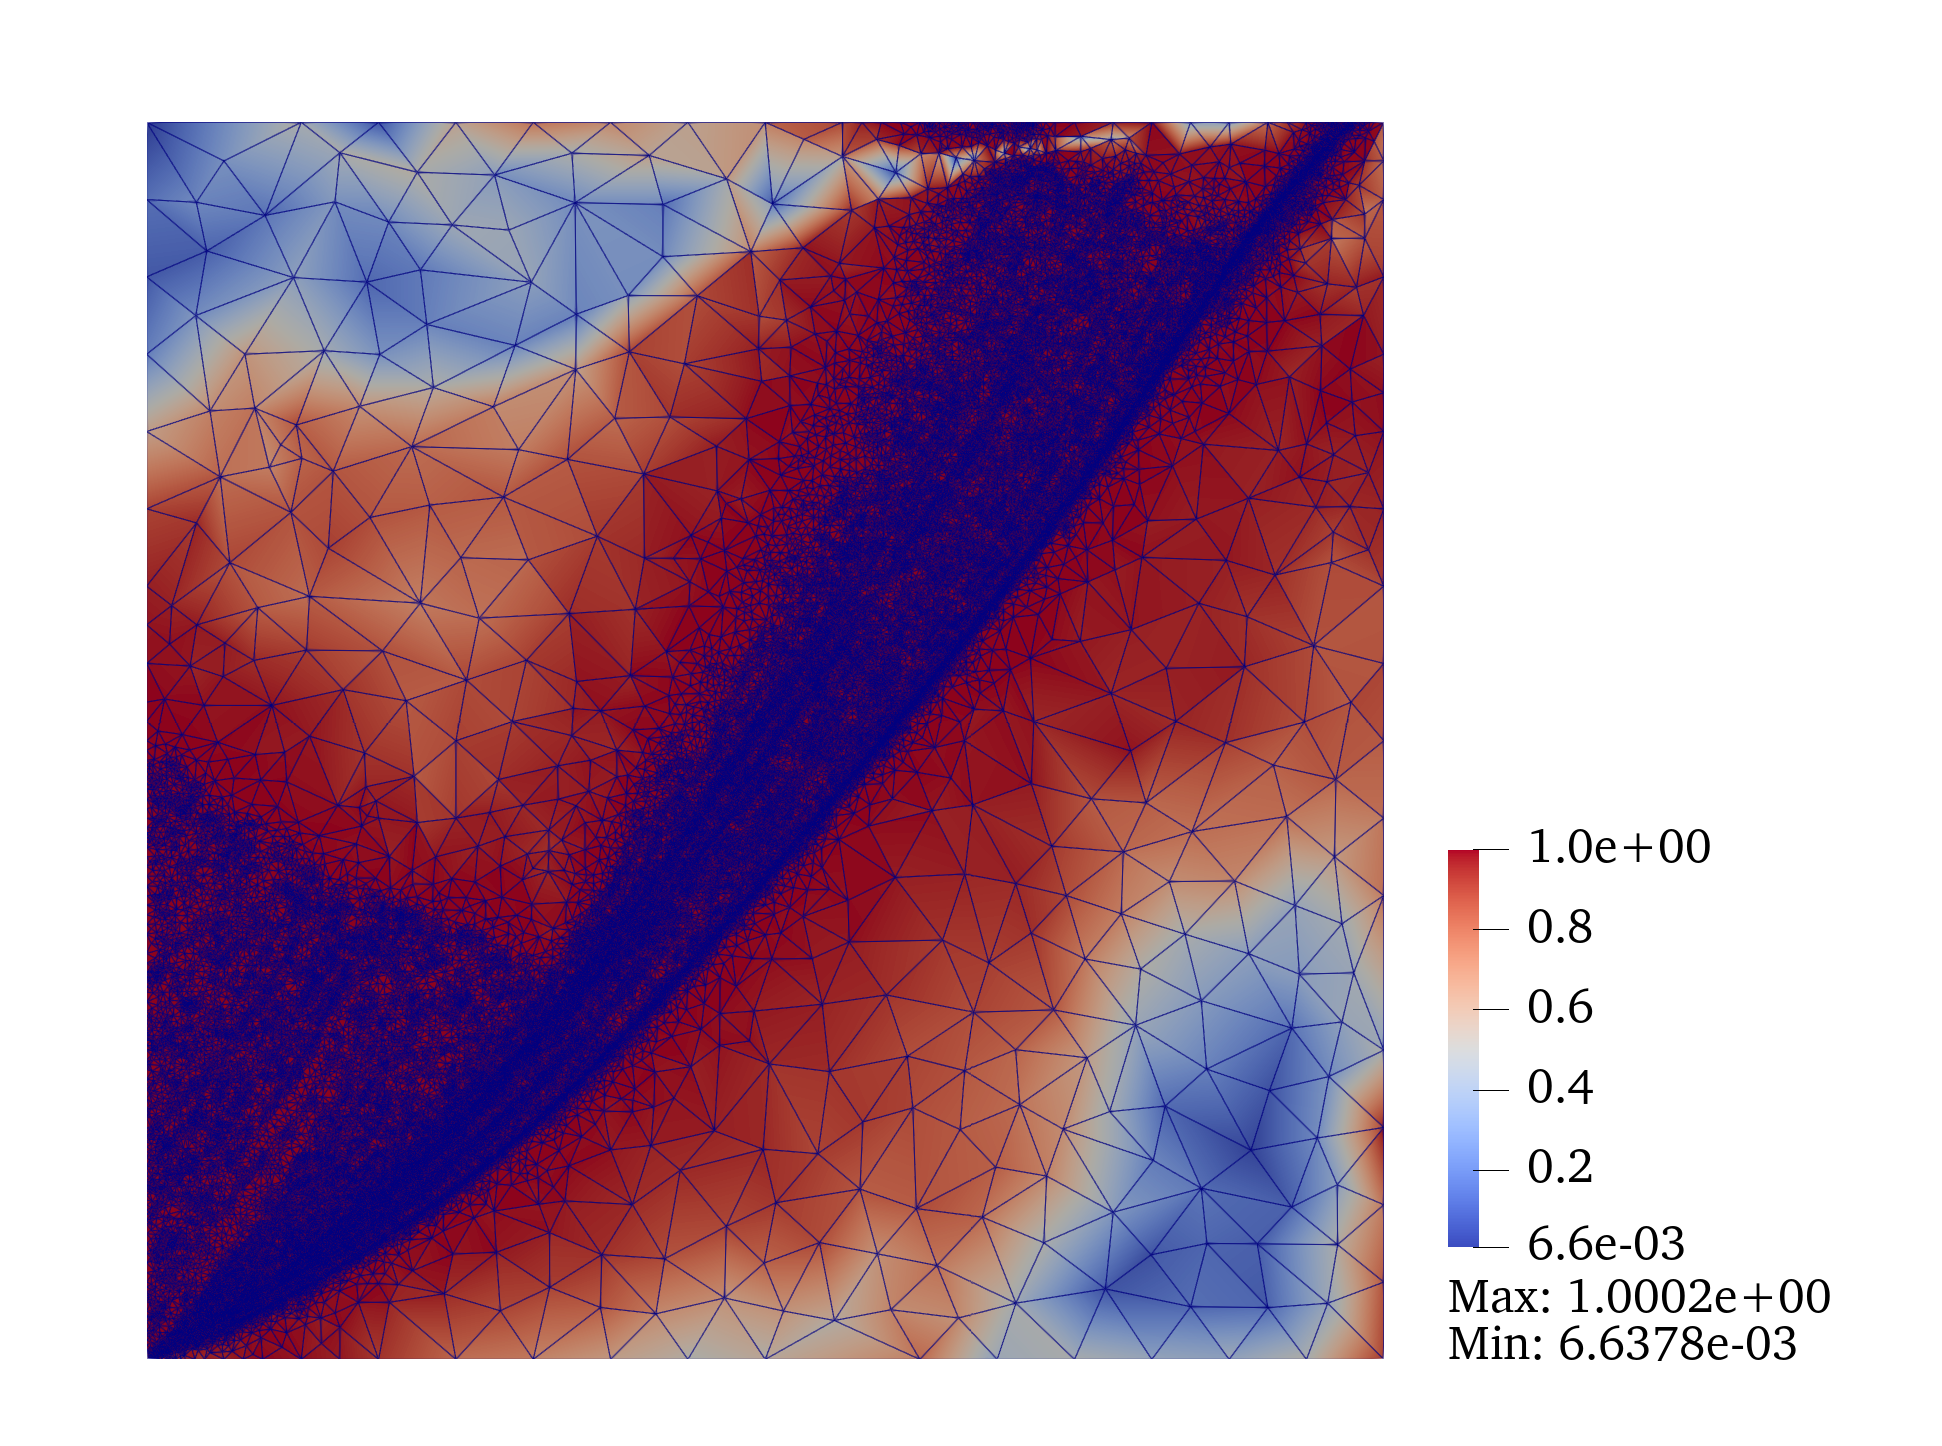
\includegraphics[width=0.9\textwidth]{figures/Res_To_Date/VCSM_Tresca stress.png}
  \caption{AMR mesh of the vertical cut problem in plane strain}
  \label{fig:VC_AMR}
\end{figure}

We may observe from Figure~\ref{fig:VC_AMR} that the refined zone matches with the slip-line zone reported in previous work by Martin~\cite{Martin_2011}. 


\subsubsection{Discussion}

After examining the three 2D benchmark problems individually, we summarize the overall timing performance of the solvers in Figure~\ref{fig:2DTimecomp}. The figure compares the time to solution of ADMM, MOSEK, and Gurobi as the problem size increases for the rigid platen, strip footing, and vertical cut problems. Gurobi is often faster than MOSEK for smaller problem instances, but its performance deteriorates significantly for larger problems. In contrast, the proposed ADMM solver consistently achieves the shortest solution times while maintaining close agreement with the IPM solutions, with the absolute difference in the computed collapse multiplier remaining below approximately $10^{-4}$.  This speedup is primarily attributed to the substantially lower cost per ADMM iteration compared with that of the IPM solvers, together with the fact that the number of ADMM iterations increases only moderately as the problem size grows.





The irregular spikes observed in the MOSEK timings for the rigid platen and strip footing problems are primarily attributed to a larger number of interior-point iterations required for those particular cases.



Specifically, we investigate the individual effects of the two proposed acceleration strategies, namely warm-starting (WS) and active-cone identification (CI). Figure~\ref{fig:2DTimecomp} compares the runtime of the proposed ADMM solver against variants employing WS or CI individually, thereby illustrating the contribution of each technique to the overall solver performance.


\paragraph{Effect of warm-starting}

Figure~\ref{fig:2DTimecomp} shows that the ADMM+WS variant achieves runtimes close to those of the proposed ADMM solver for the smaller problem instances. As the problem size increases, however, the performance gap becomes more apparent. Warm-starting primarily improves the initial stage of the optimization by providing an iterate that is already close to the solution of the refined problem. This reduces the transient phase of ADMM convergence and, consequently, the number of iterations required to reach the prescribed stopping tolerances. Nevertheless, warm-starting does not directly address the slower convergence that may arise during the later stages of the iteration process.

\paragraph{Effect of active-cone identification}

The ADMM+CI variant is generally slower than both ADMM+WS and the proposed ADMM solver in the cases considered, although it remains faster than the commercial IPM solvers. Its effect is complementary to that of warm-starting. Whereas warm-starting improves the initial iterate, active-cone identification modifies the penalty weights associated with SOC blocks that are likely to be active at the solution. By placing greater emphasis on these constraints, the method improves the enforcement of the locally governing part of the feasible set and accelerates late-stage convergence.

This behaviour becomes increasingly important for the larger problem instances. As shown in Figure~\ref{fig:2DTimecomp}, the proposed ADMM solver, which combines WS and CI, outperforms the WS-only variant for the largest cases considered. The results therefore suggest that warm-starting and active-cone identification act on different phases of the ADMM iteration: warm-starting reduces the initial transient, while active-cone identification improves convergence as the iterates approach the solution. Their combination provides a more consistent reduction in the overall time-to-solution, while the required number of ADMM iterations remains approximately insensitive to the problem size over the range considered.

\paragraph{Effect of warm-starting in adaptive mesh refinement}

The structured-mesh experiments above provide a controlled setting for evaluating the algorithmic effect of warm-starting across problem sizes. In practical FELA analyses, however, mesh refinement is more naturally performed sequentially through adaptive refinement, producing a hierarchy of closely related but non-identical optimization problems. This setting provides a distinct test of the proposed transfer strategy, since both the mesh topology and local element sizes evolve between successive solves.

To assess the effectiveness of warm-starting in this more representative workflow, we compare the final AMR solve with and without transferring the solution from the preceding mesh. The results are reported in Table~\ref{tab:2DWS_AMR}. Across the three 2D benchmarks, warm-starting reduces both the iteration count and the overall solution time while producing essentially unchanged collapse multipliers. These results confirm that the proposed warm-starting strategy remains effective not only in controlled structured-mesh comparisons, but also in a genuinely hierarchical adaptive-refinement setting.




\begin{figure}[htbp]
  \centering
  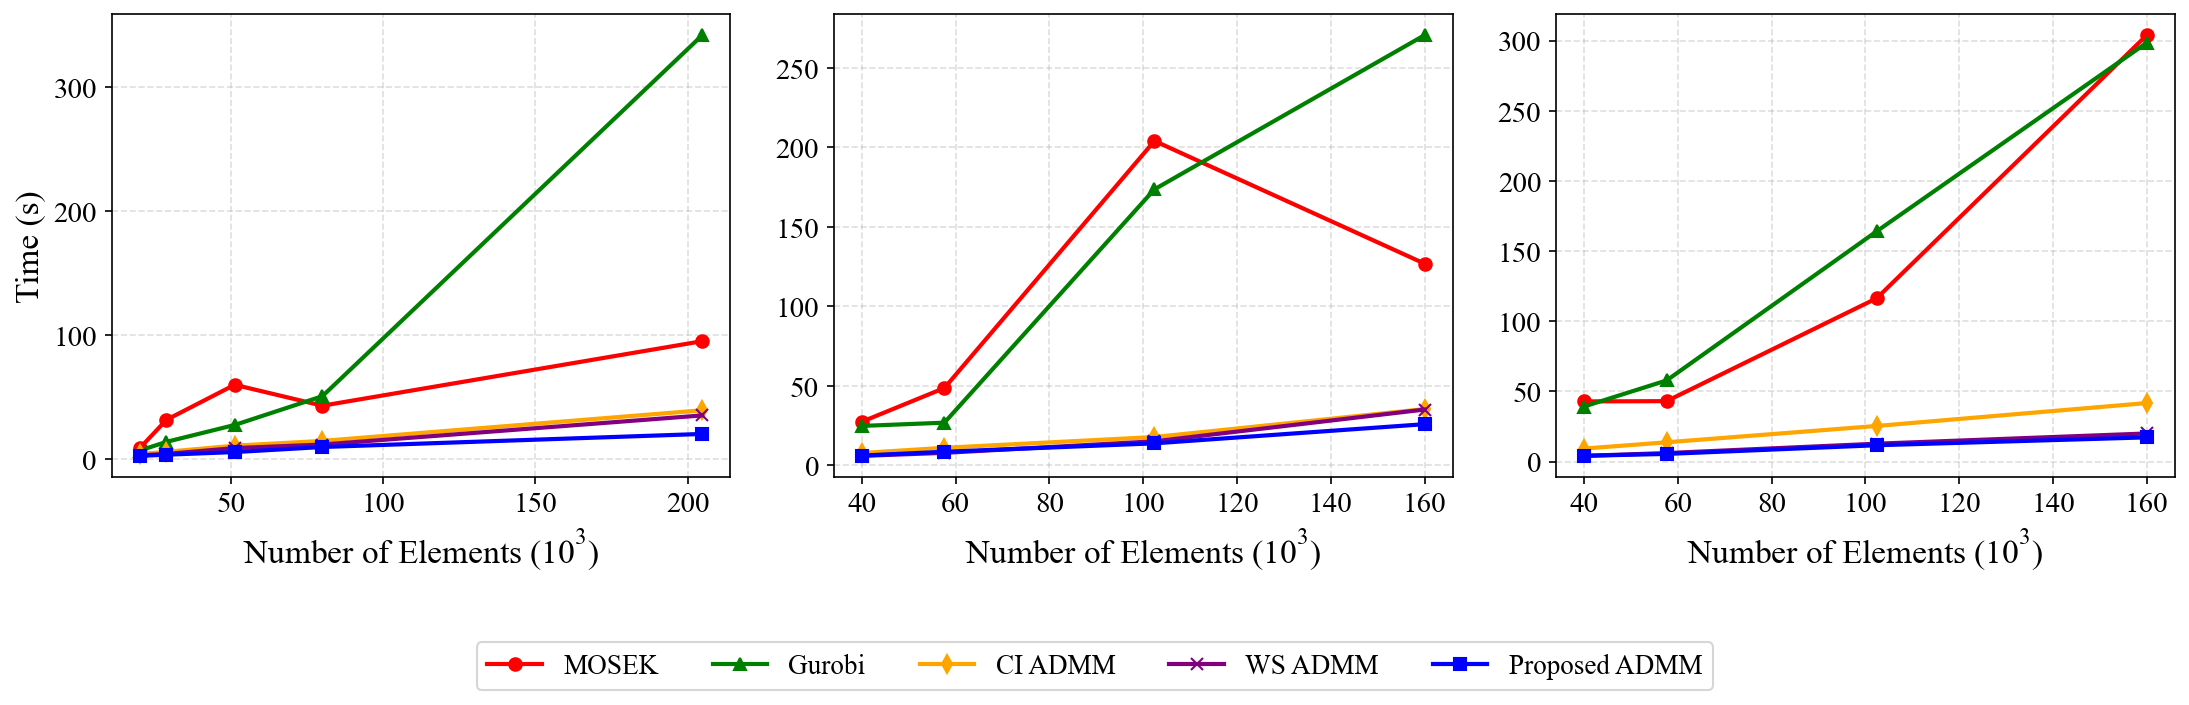
\includegraphics[width=0.95\textwidth]{figures/Res_To_Date/TC_ALL.png}
  \caption{Timing comparison of different ADMM implementations against IPM solvers in 2D benchmark problems using structured mesh (From left to right: Rigid platen, strip footing, vertical cut)}
  \label{fig:2DTimecomp}
\end{figure}
\begin{table}[htbp] 
\centering 
\caption{Performance enhancement achieved with warm-starting using adaptive refined mesh} 
\label{tab:2DWS_AMR} 
 
\begin{tabular}{@{}C{2.1cm}C{1.8cm}C{1.8cm}C{2cm}C{1.5cm}C{1.6cm}C{2.1cm}C{1.6cm}@{}} 
\toprule 
\textbf{Problem type} &
\multicolumn{2}{c}{\textbf{Problem size}} & 
\textbf{Warm starting} & 
\textbf{Solve time (s)} & 
\textbf{Iterations} & 
\textbf{Load multiplier} & 
\textbf{Speedup} 
\tabularnewline 
\cmidrule(lr){2-3} 
& 
\textbf{$N_{\mathrm{elem}}(\times 10^3)$} & 
\textbf{$N_{\mathrm{var}}(\times 10^6)$} & 
& 
& 
& 
& 
\tabularnewline 
\midrule 
 
\multirow{2}{*}{Rigid Platen} 
& \multirow{2}{*}{362.49} 
& \multirow{2}{*}{3.26} 
& Yes & 52.24 & 400 & 2.42681 & \multirow{2}{*}{16\%} \tabularnewline 
& & & No  & 61.91 & 460 & 2.42689 & \tabularnewline 
 
\addlinespace 
 
\multirow{2}{*}{Strip Footing} 
& \multirow{2}{*}{553.50} 
& \multirow{2}{*}{4.98} 
& Yes & 75.15 & 400 & 5.13648 & \multirow{2}{*}{40\%} \tabularnewline 
& & & No  & 125.35 & 620 & 5.13668 & \tabularnewline 
 
\addlinespace 
 
\multirow{2}{*}{Vertical Cut} 
& \multirow{2}{*}{452.23} 
& \multirow{2}{*}{4.07} 
& Yes & 77.56 & 460 & 3.77522 & \multirow{2}{*}{30\%} \tabularnewline 
& & & No  & 110.90 & 660 & 3.77549 & \tabularnewline 
 
\bottomrule 
\end{tabular} 
 
\vspace{0.5em} 
\end{table}


\subsection{3D Benchmark Problems}

\subsubsection{Rigid Platen Problem}
\paragraph{Problem setup} 


This example considers the 3D compression of a von Mises soil block between two rigid platens, as illustrated in Figure~\ref{fig:3D2PR_CS}. The soil domain has dimensions $L \times L \times 0.5L$. The soil is assumed to obey the von-Mises yield criterion. We exploit symmetry on the lower, frontal and diagonal boundaries, while the upper rigid platen is subjected to a vertical live load $F_{\mathrm{live}}$. The soil-platen interfaces are taken to be fully rough. The remaining right boundary is left free. By exploiting symmetry, only one sixteenth of the model needs to be analysed.

\begin{figure}[htbp]
  \centering
  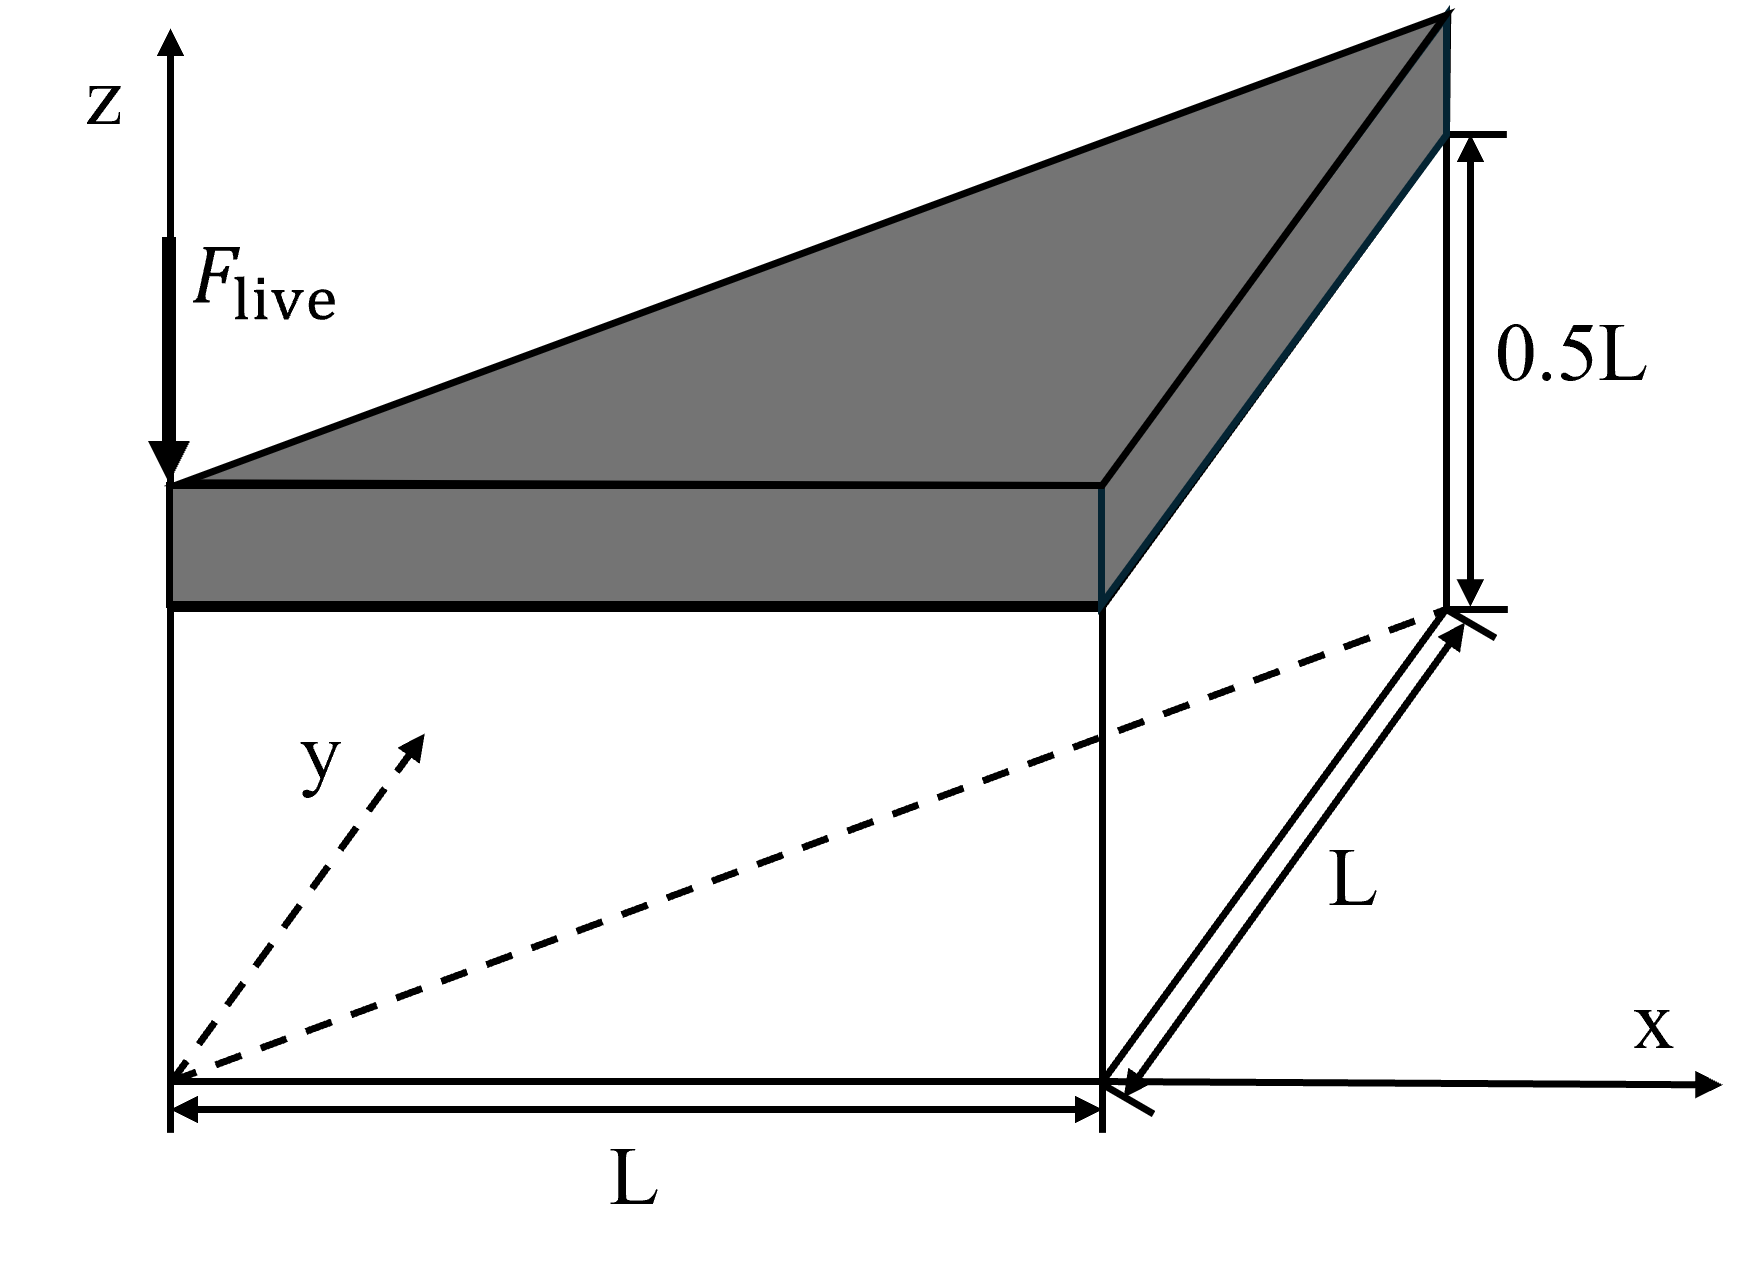
\includegraphics[width=0.44\textwidth]{figures/Res_To_Date/3D2PR_config.png}
  \hfill
  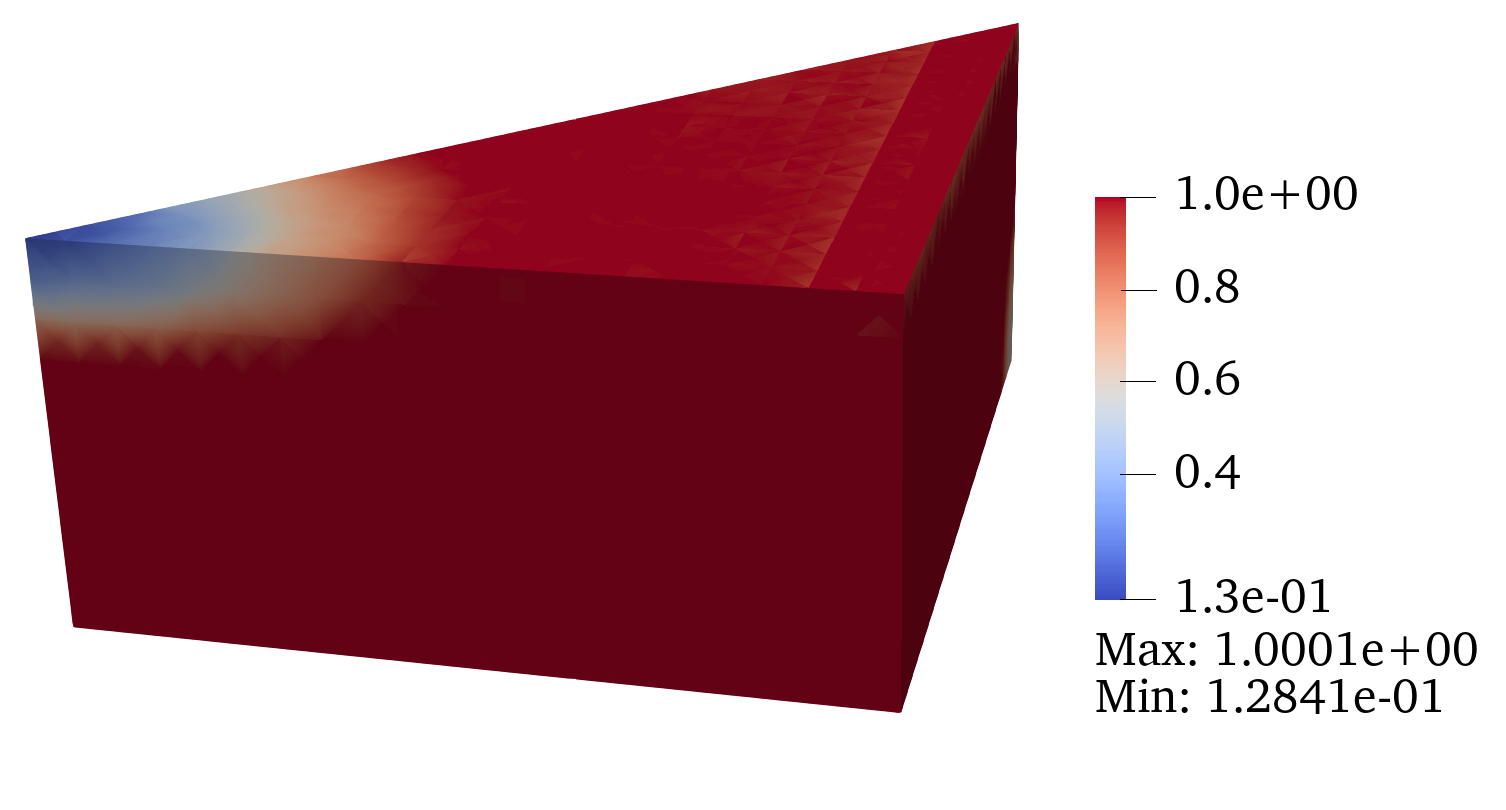
\includegraphics[width=0.55\textwidth]{figures/Res_To_Date/3D2PR_solution.png}
  \caption{3D rigid platen problem. \textbf{Left}: physical configuration; \textbf{Right}: solution of the yield function using a structured mesh}
  \label{fig:3D2PR_CS}
\end{figure}

\paragraph{Benchmark comparison using structured mesh} 

\begin{table}[htbp]
\centering
\caption{Solver performance comparison on the 3D rigid platen benchmark for different mesh discretizations}
\label{tab:3D2PR_table}

\begin{tabular}{@{}C{1.7cm}C{1.7cm}C{1.5cm}C{2.0cm}C{2.3cm}C{2.3cm}C{2.3cm}@{}}
\toprule
\multicolumn{2}{c}{\textbf{Problem size}} &
\textbf{Solver} &
\textbf{Solve time (s)} &
\textbf{Collapse multiplier} &
\textbf{Iterations} &
\textbf{Time-per-iter (s)}
\tabularnewline

\cmidrule(lr){1-2}

\textbf{$N_{\mathrm{elem}}(\times 10^3)$} &
\textbf{$N_{\mathrm{var}}(\times 10^6)$} &
&
&
&
&
\tabularnewline

\midrule

\multirow{3}{*}{6}
& \multirow{3}{*}{0.148}
& MOSEK		& 8.84	& 2.08904 & 24 & 0.37 \tabularnewline
& & Gurobi 	& 10.15  	& 2.08905 & 17 & 0.60 \tabularnewline
& & ADMM 	& 4.33 	& 2.08844 & 220 & 0.019 \tabularnewline

\addlinespace

\multirow{3}{*}{24.6}
& \multirow{3}{*}{0.589}
& MOSEK  		& 96.63	& 2.09546 & 33 & 2.93 \tabularnewline
& & Gurobi	& 147.24	& 2.09546 & 16 & 9.20\tabularnewline
& & ADMM   	& 22.33 	& 2.09526 & 220 & 0.10\tabularnewline

\addlinespace

\multirow{3}{*}{48}
& \multirow{3}{*}{1.152}
& MOSEK  & 371.2 & 2.09755 & 39 & 9.52 \tabularnewline
& & Gurobi & 618.31 & 2.09755 & 17 & 36.37 \tabularnewline
& & ADMM   & 61.99 & 2.09708 & 180 & 0.34\tabularnewline

\bottomrule
\end{tabular}

\vspace{0.5em}
\end{table}

Table~\ref{tab:3D2PR_table} shows that our solver still yields a speedup, from $2.04\times$ to $5.99\times$ compared with MOSEK in 3D FELA problems. Speedup is achieved in both linear and linear elements, with the largest speedup of $5.99\times$ achieved at the largest linear case. It should be noted however, the sparsity pattern of the 3D problem differs from that of the 2D problems, thereby incurring a substantial increase in the number of fill-ins in direct factorization, which limited the maximum problem size we can explore.

\subsubsection{Square Footing Problem}

\paragraph{Problem setup}
Similar to the 2D strip footing problem, the square footing problem considers a rigid footing resting on the surface of a soil body. By exploiting symmetry, only one eighth of the full domain is modelled. Symmetry boundary conditions are imposed on the diagonal plane and the frontal plane. The rigid footing is located at the top-left corner of the computational domain, corresponding to the symmetric portion of the full square footing. The footing side length is set to one fifth of the characteristic length of the soil body, i.e. $L$ for a soil domain of characteristic length $5L$. The bottom boundary and the far-field lateral boundary on the right-hand side are fixed, while the remaining external boundaries are left free unless constrained by symmetry or footing contact conditions.

No analytical lower-bound solution appears to be available for the square or rectangular footing problem. However, da Silva and Salgado~\cite{daSilva_2020, Salgado_2004} investigated this problem with Tresca criterion using FELA and with linear stress elements. Salgado~\cite{Salgado_2004} reported a lower-bound solution of 5.523 using a tailored mesh with thin elements near the footing edge, whereas da Silva~\cite{daSilva_2020} obtained a lower-bound solution of 5.625 on a very fine structured mesh.

\begin{figure}[htbp]
  \centering
  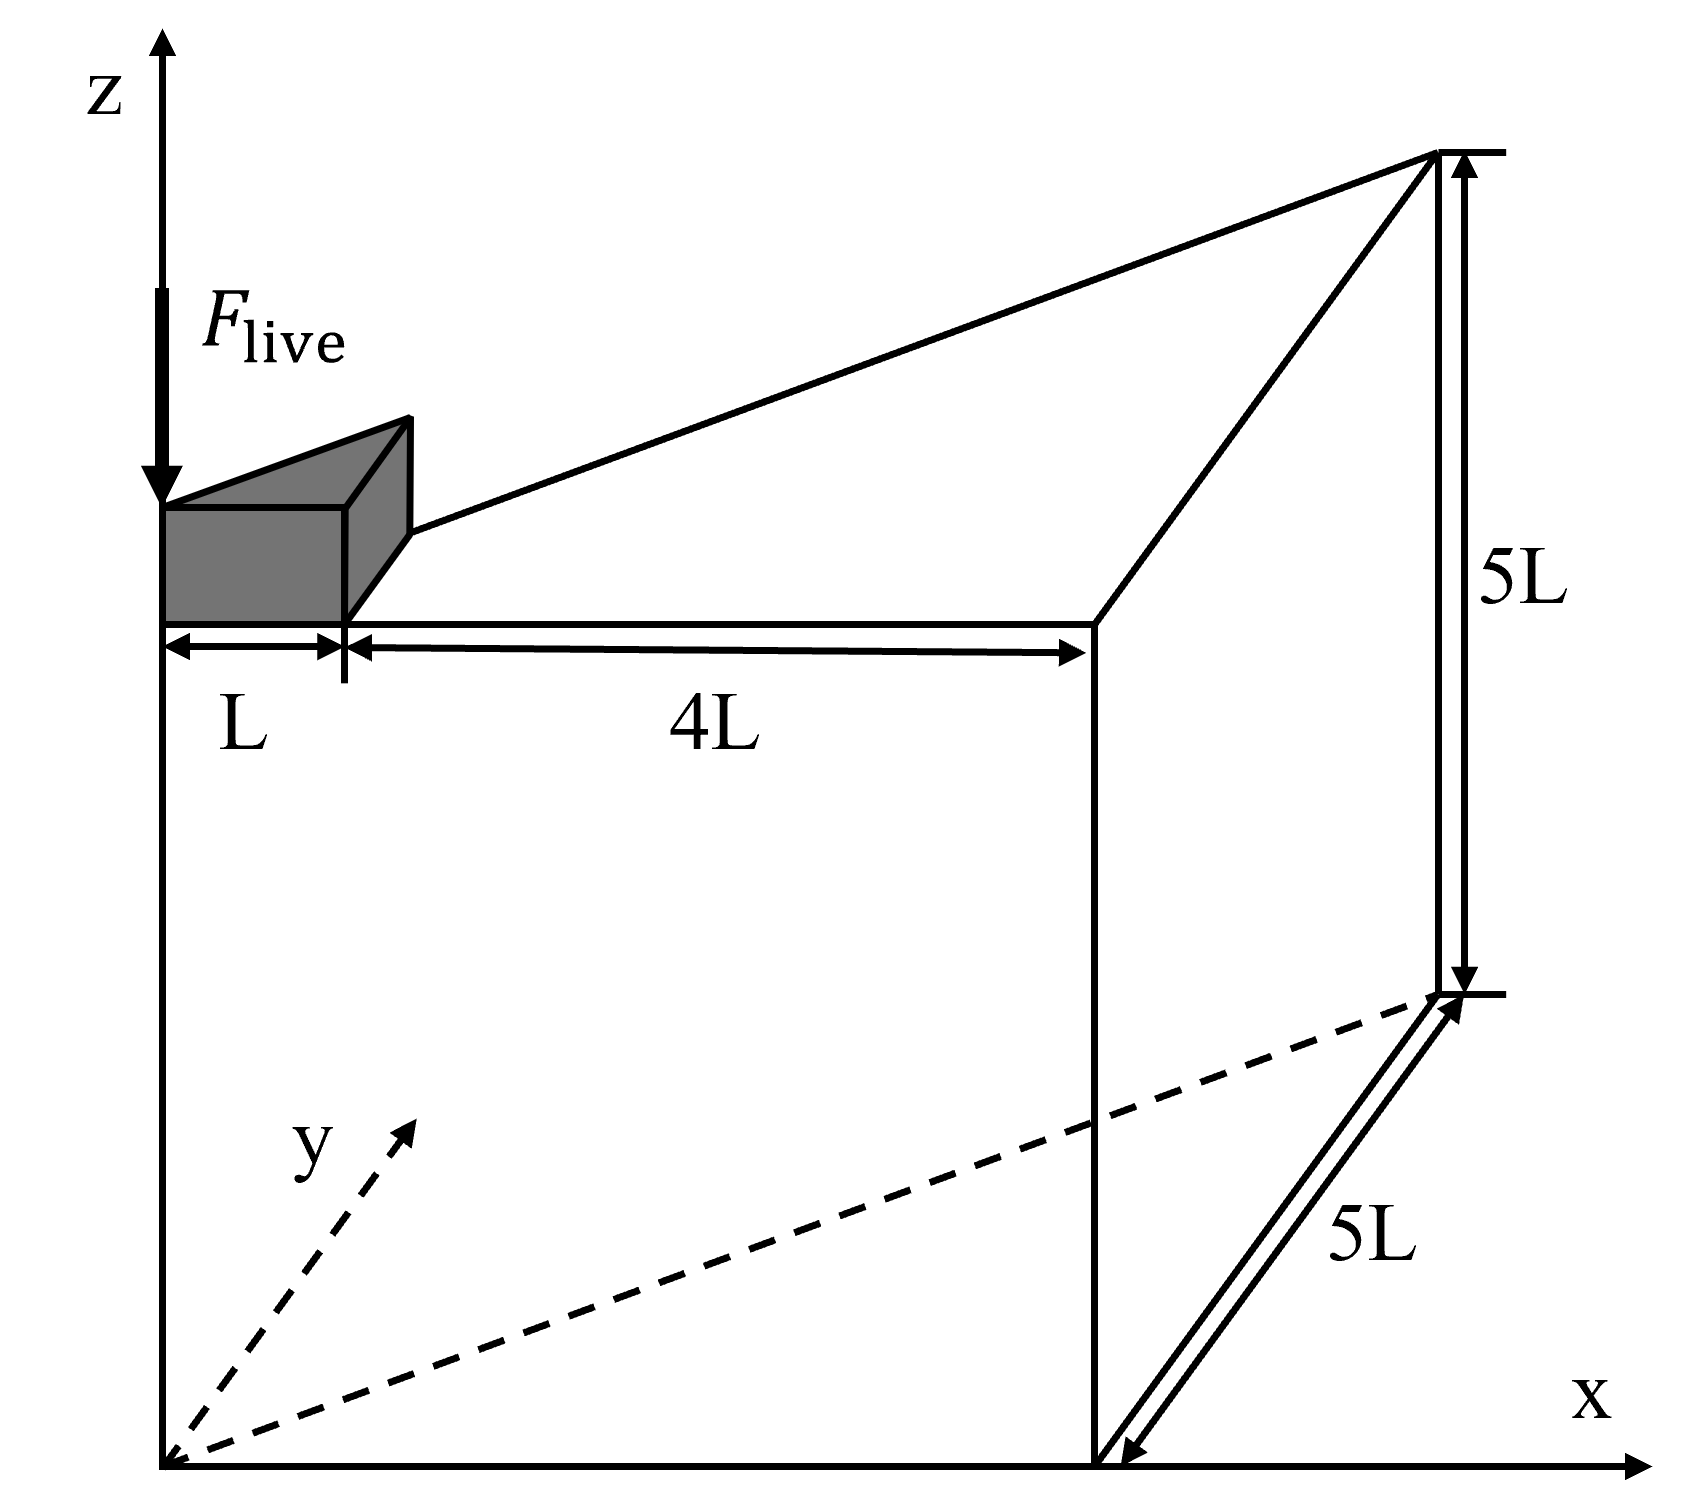
\includegraphics[width=0.46\textwidth]{figures/Res_To_Date/3DSF_config.png}
  \hfill
  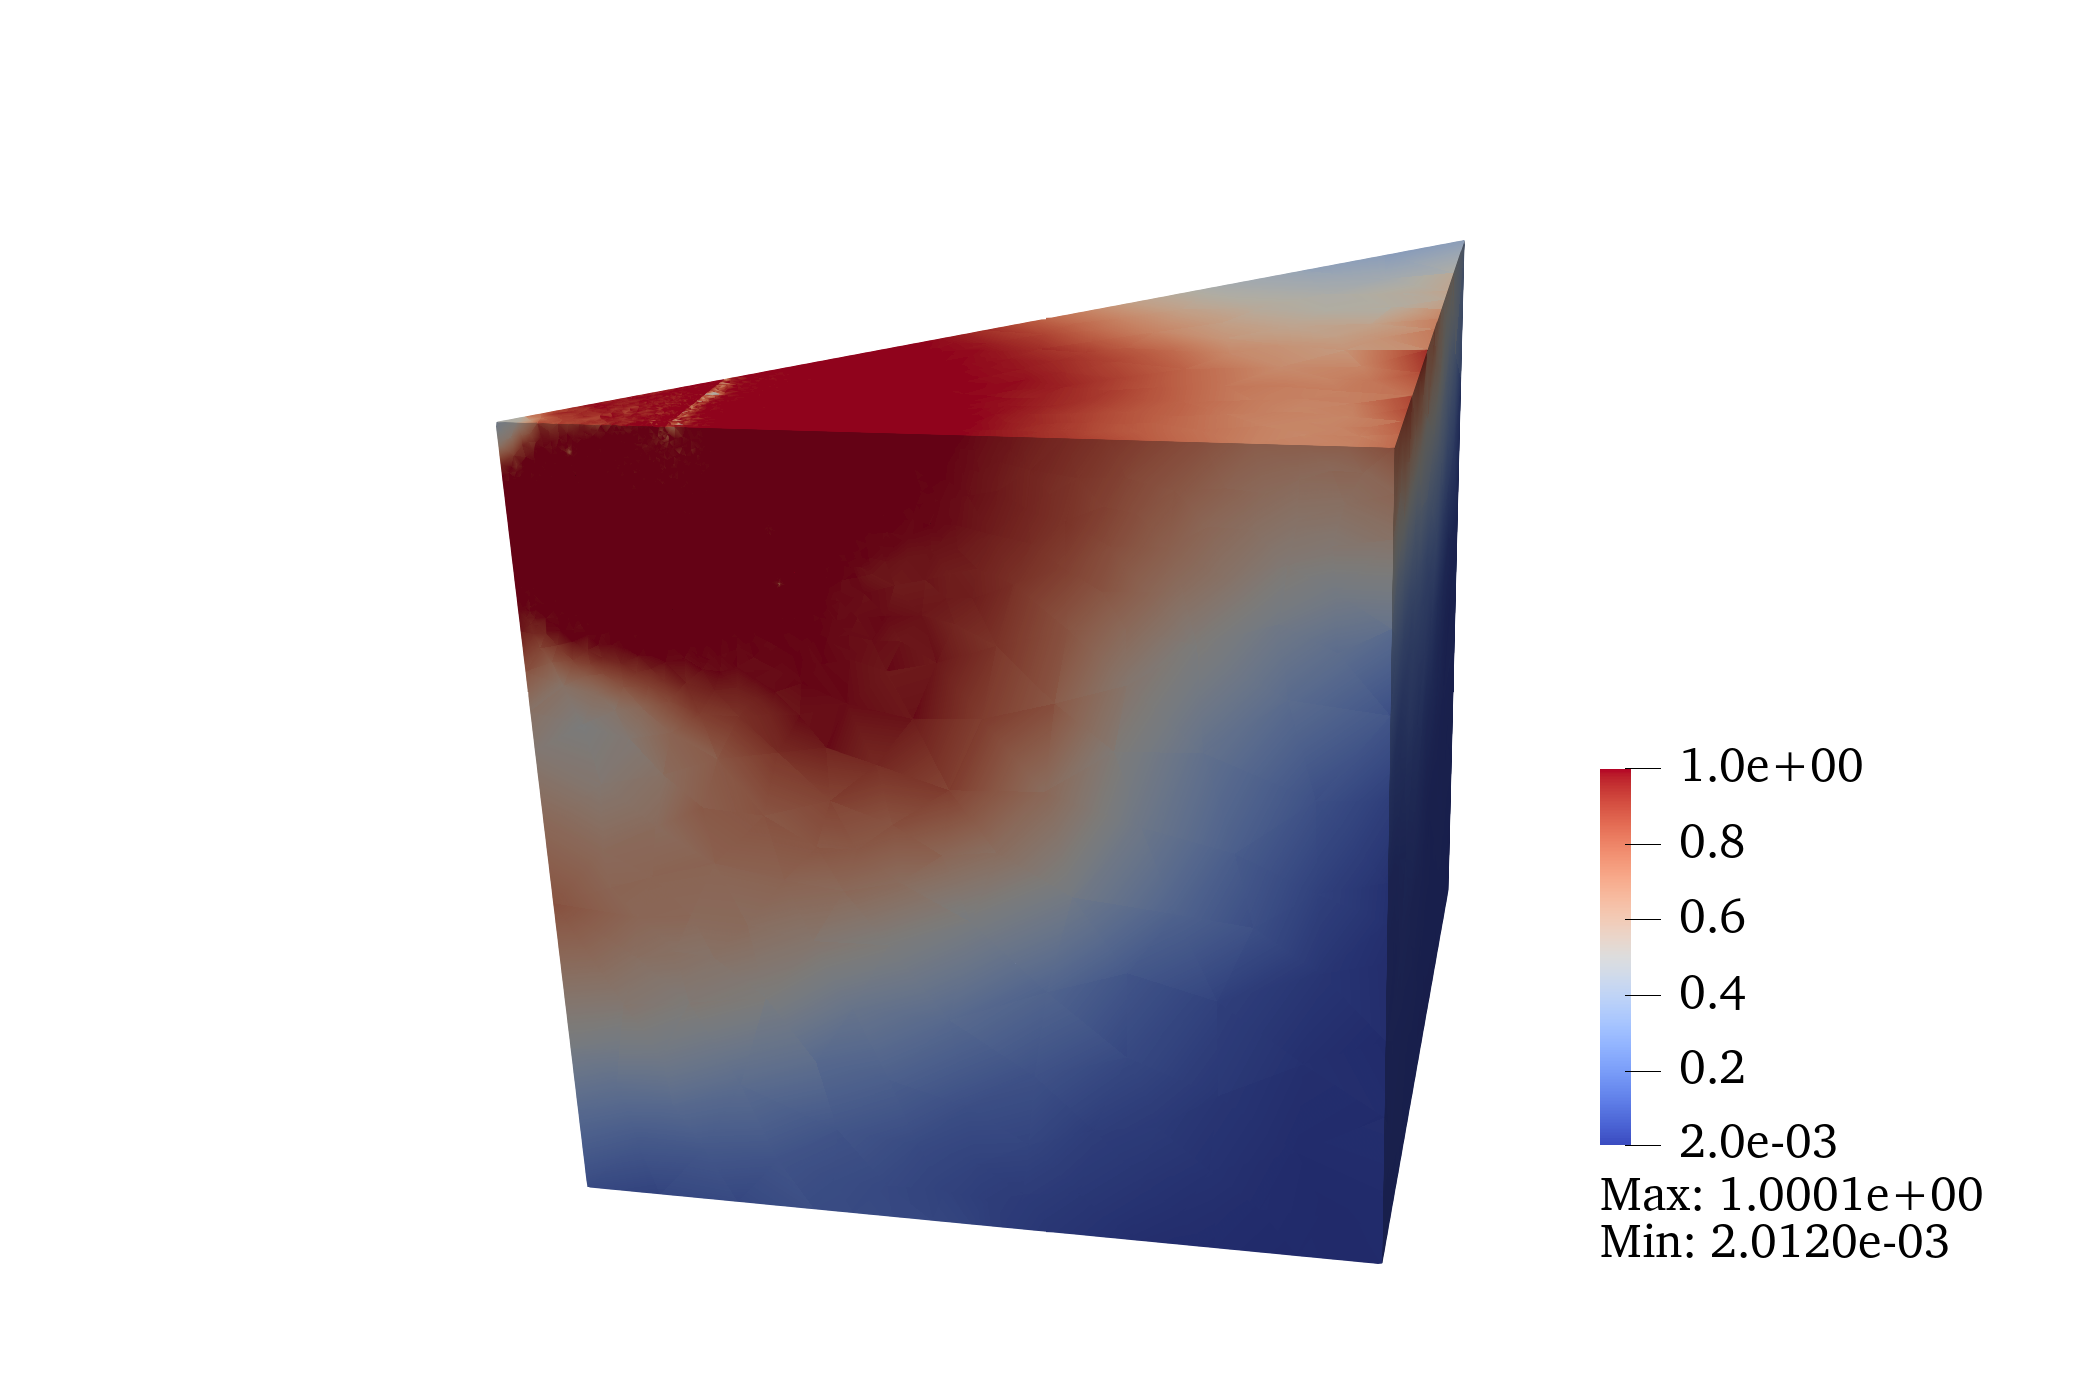
\includegraphics[width=0.53\textwidth]{figures/Res_To_Date/3DSF_solution_AMR.png}
  \caption{3D square footing problem. \textbf{Left}: physical configuration; \textbf{Right}: solution of the yield function using a refined quadratic mesh}
  \label{fig:3DSF_CS}
\end{figure}


\paragraph{Benchmark comparison using structured mesh}

The performance of the proposed 3D ADMM solver is first assessed on structured meshes and compared against MOSEK. The results are summarized in Table~\ref{tab:3DSF_table}. Similar to the previous benchmarks, both the time-to-solution and the computed collapse multiplier are reported.

\begin{table}[htbp]
\centering
\caption{Solver performance comparison on the 3D square footing benchmark for different mesh discretizations}
\label{tab:3DSF_table}

\begin{tabular}{@{}C{1.7cm}C{1.7cm}C{1.5cm}C{2.0cm}C{2.3cm}C{2.3cm}C{2.3cm}@{}}
\toprule
\multicolumn{2}{c}{\textbf{Problem size}} &
\textbf{Solver} &
\textbf{Solve time (s)} &
\textbf{Collapse multiplier} &
\textbf{Iterations} &
\textbf{Time-per-iter (s)}
\tabularnewline

\cmidrule(lr){1-2}

\textbf{$N_{\mathrm{elem}}(\times 10^3)$} &
\textbf{$N_{\mathrm{var}}(\times 10^6)$} &
&
&
&
&
\tabularnewline

\midrule

\multirow{3}{*}{12}
& \multirow{3}{*}{0.288}
& MOSEK  		& 20.87	& 5.22710 & 27	&  0.77\tabularnewline
& & Gurobi 	& 31.93	& 5.22716 & 16 	&  1.99\tabularnewline
& & ADMM   	& 17.65	& 5.22694 & 420 & 0.042 \tabularnewline

\addlinespace

\multirow{3}{*}{96}
& \multirow{3}{*}{2.304}
& MOSEK  & 937.53 & 5.36728 & 32  & 29.29  \tabularnewline
& & Gurobi$^{\dagger}$ &  --    & --      & -- & $\approx$ 200 \tabularnewline
& & ADMM   & 538.21 & 5.36173 & 540 & 0.99 \tabularnewline

\bottomrule
\end{tabular}

\begin{minipage}{0.98\linewidth}
\footnotesize
$^{\dagger}$ Gurobi did not complete the larger problem. The reported estimated time per iteration was approximately \(200\,\mathrm{s}\); therefore, the run was terminated due to the excessive computational time.

\end{minipage}

\vspace{0.5em}
\end{table}




Table~\ref{tab:3DSF_table} shows that across all tested cases, the relative discrepancy between the two solvers remains small, confirming that the proposed ADMM can recover high-quality LB solutions for this 3D benchmark. Refining the linear mesh to $96\times10^3$ elements increases the collapse multiplier to about $5.36$. This trend is consistent with the expected convergence of lower-bound FELA solutions under mesh refinement.

In terms of computational performance, the ADMM solver remains faster than MOSEK, with speedups ranging from approximately $1.27\times$ to $2.61\times$. These speedups are more modest than those observed in the 2D strip footing benchmark and in the 3D rigid platen problem. This is because the square footing problem produces a more demanding three-dimensional KKT system, for which sparse direct factorization introduces substantially more fill-in. Consequently, the cost of storing and applying the factorized matrices becomes a dominant part of the total solution time. The benchmark therefore highlights both the robustness of the proposed solver and the memory-related scalability bottleneck of the current direct-solve implementation in 3D.

\paragraph{Adaptive mesh refinement}

Here we demonstrate the ability of our methodology to obtain an accurate LB solution in 3D. We were able to obtain an accurate LB solution of $\beta = 5.40200$. This solution is obtained with 8 adaptive mesh refinements with 0.18 million linear stress elements, and the adaptive mesh obtained is shown in Figure~\ref{fig:3DSF_AMR_SOL}.

\begin{figure}
\centering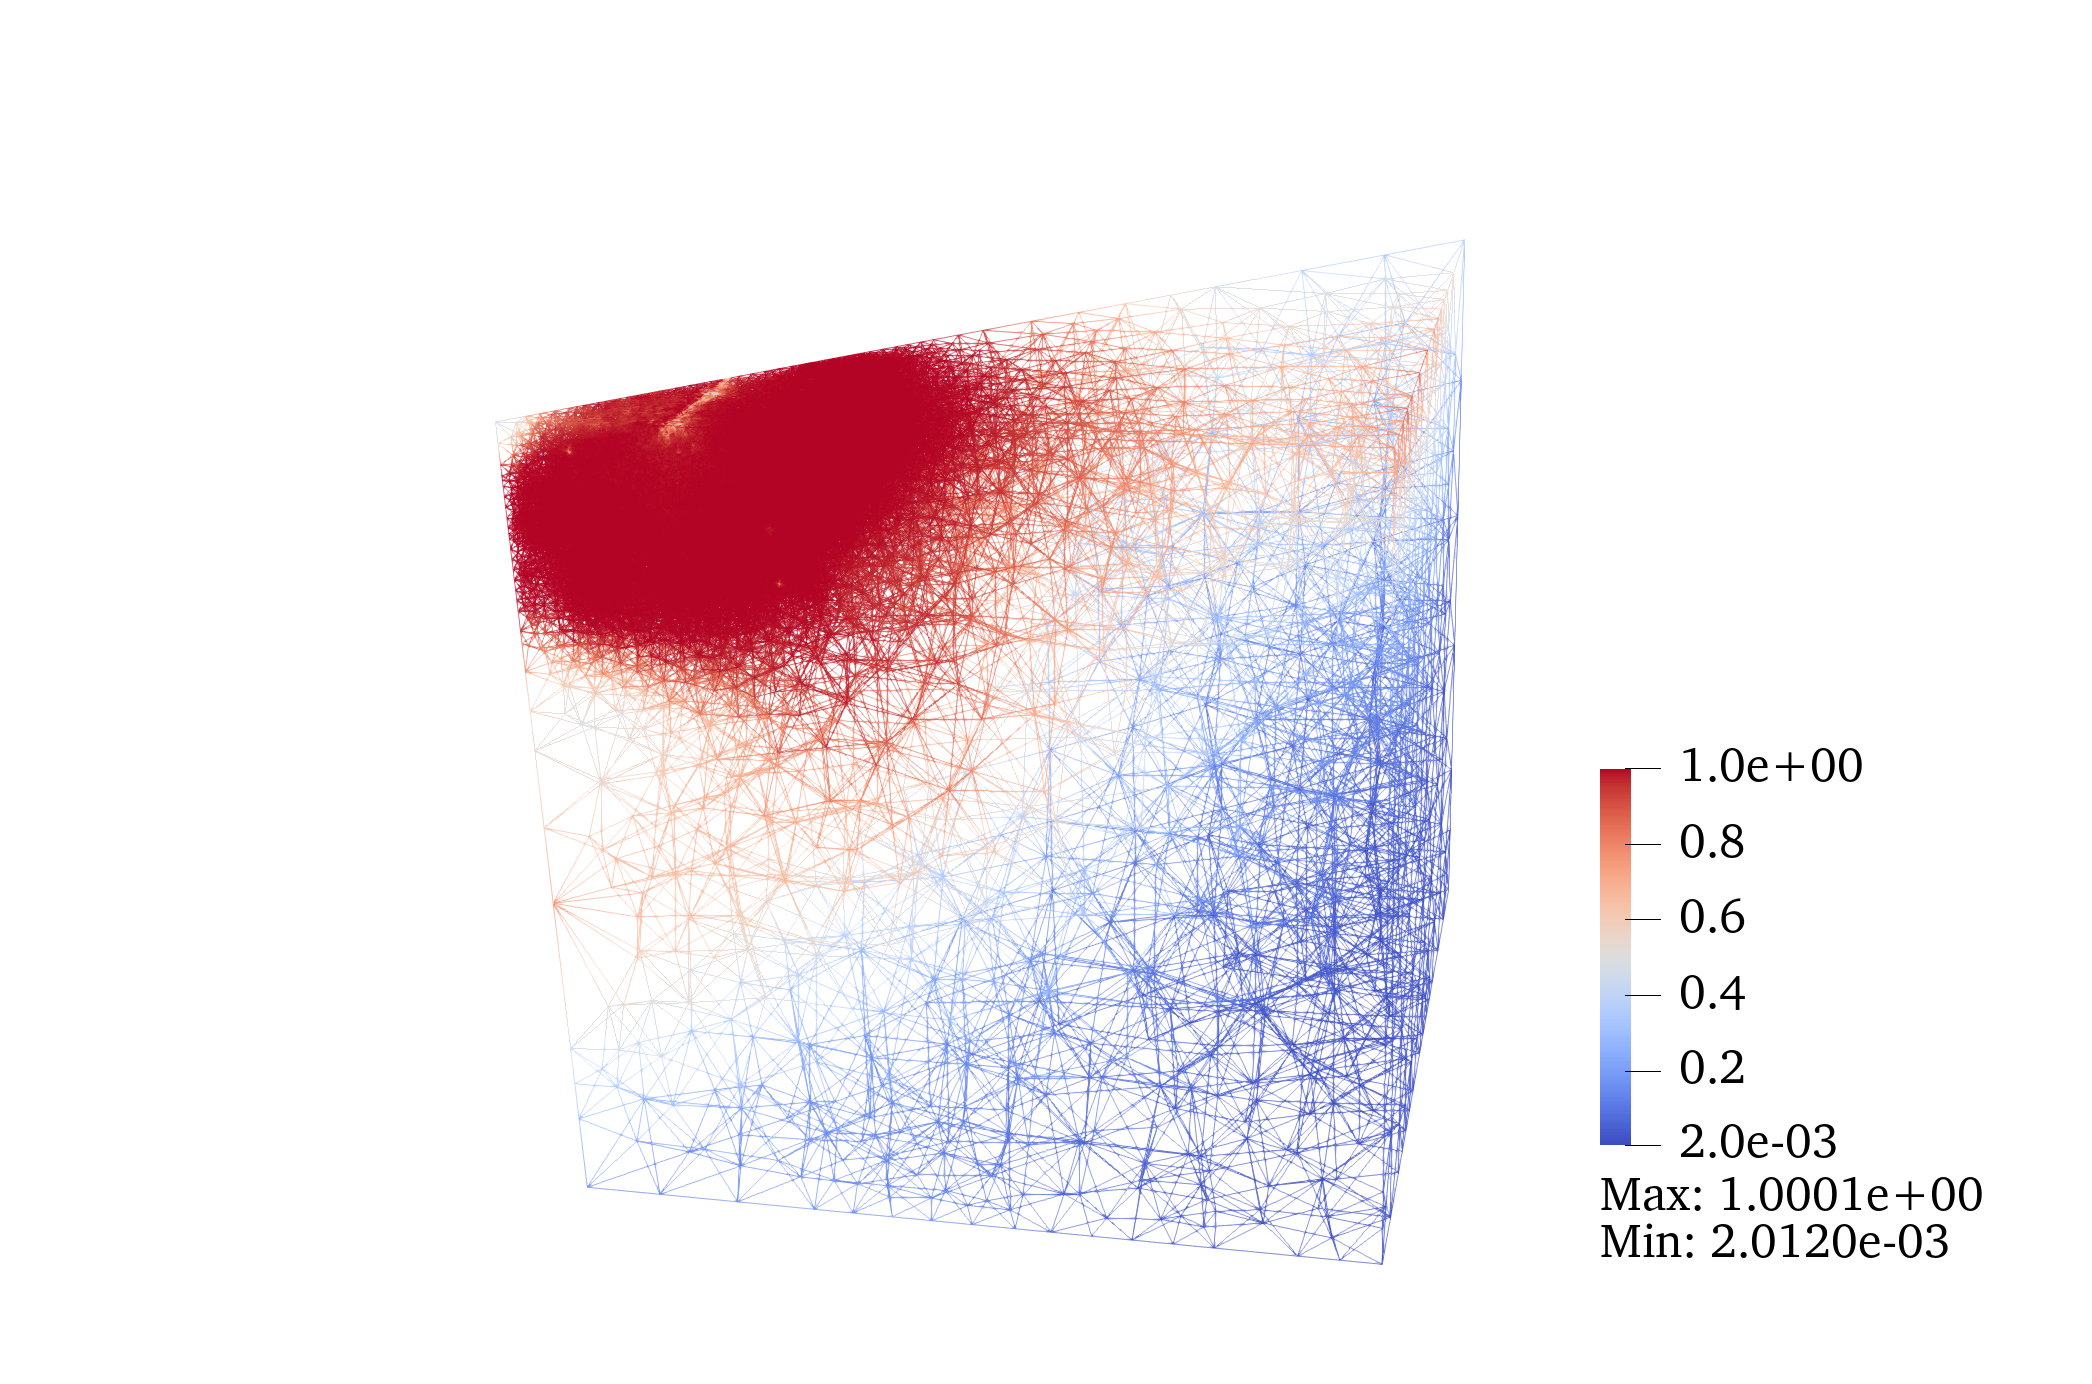
\includegraphics[width=0.8\textwidth]{figures/Res_To_Date/AMR_A1000.png} 
\caption{AMR result of the square footing problem}
\label{fig:3DSF_AMR_SOL}
\end{figure}

The AMR result demonstrates that the proposed framework can be extended to challenging three-dimensional FELA problems and can automatically concentrate resolution in the critical yielding region as shown in the upper left corner of the soil body in Figure~\ref{fig:3DSF_AMR_SOL}. Nevertheless, the process was stopped after 8 refinements because the excessive fill-in introduced by sparse direct factorization exhausted the available GPU device memory. This limitation arises from the direct factorization-solve routine, and could potentially be alleviated in larger 3D problems by adopting an indirect, matrix-free linear solver.

\subsubsection{Vertical Cut Problem}

\paragraph{Problem Setup}

In 3D, the geometry of the cut is characterized by the aspect ratio $H/B$, where $H$ denotes the depth of the cut and $B$ denotes its width. Unless otherwise stated, we consider the case $H/B=5$, with $H=1$, $B=0.2$, and $L=2$, so that the computational domain is sufficiently large to contain the potential failure mechanism. Similar to its 2D counterpart, the soil is modelled as a von Mises material subjected to a uniform body force representing the live load. The vertical cut surface and the top surface are taken as free boundaries; the front and back diagonal surfaces are treated as symmetry planes; and the right and bottom surfaces are fixed. The physical configuration is illustrated in Figure~\ref{fig:3DVC_CS}. Exploiting symmetry, only one quarter of the soil domain is modelled.


\begin{figure}[htbp]
  \centering
  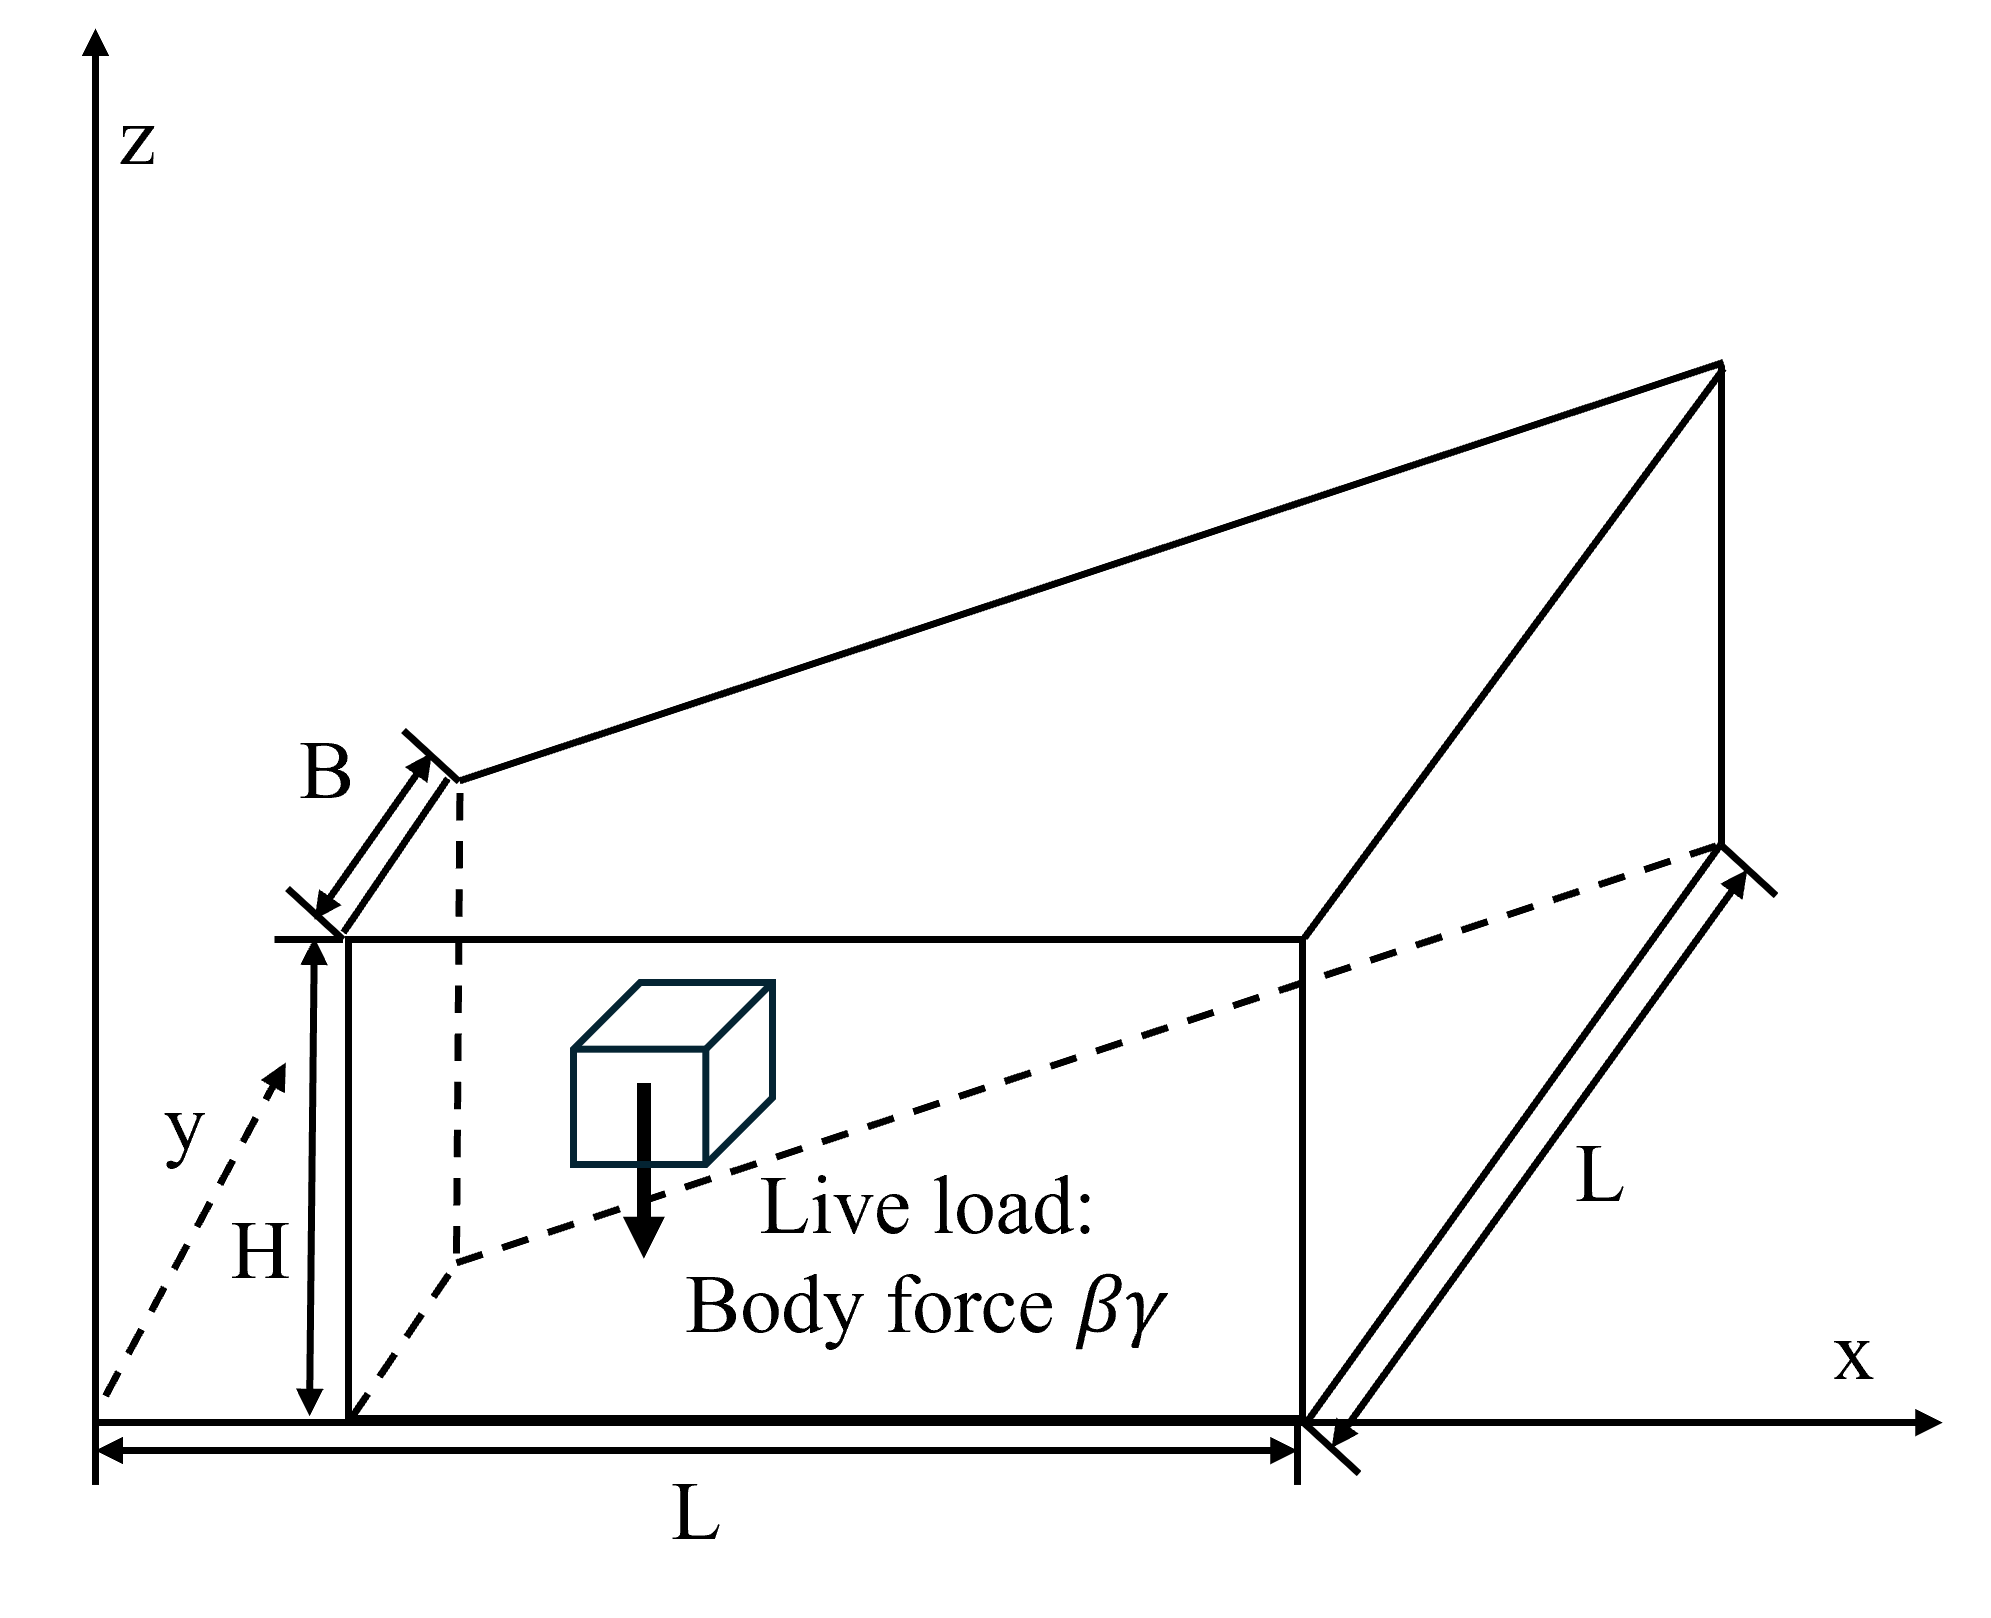
\includegraphics[width=0.44\textwidth]{figures/Res_To_Date/3DVC_config.png}
  \hfill
  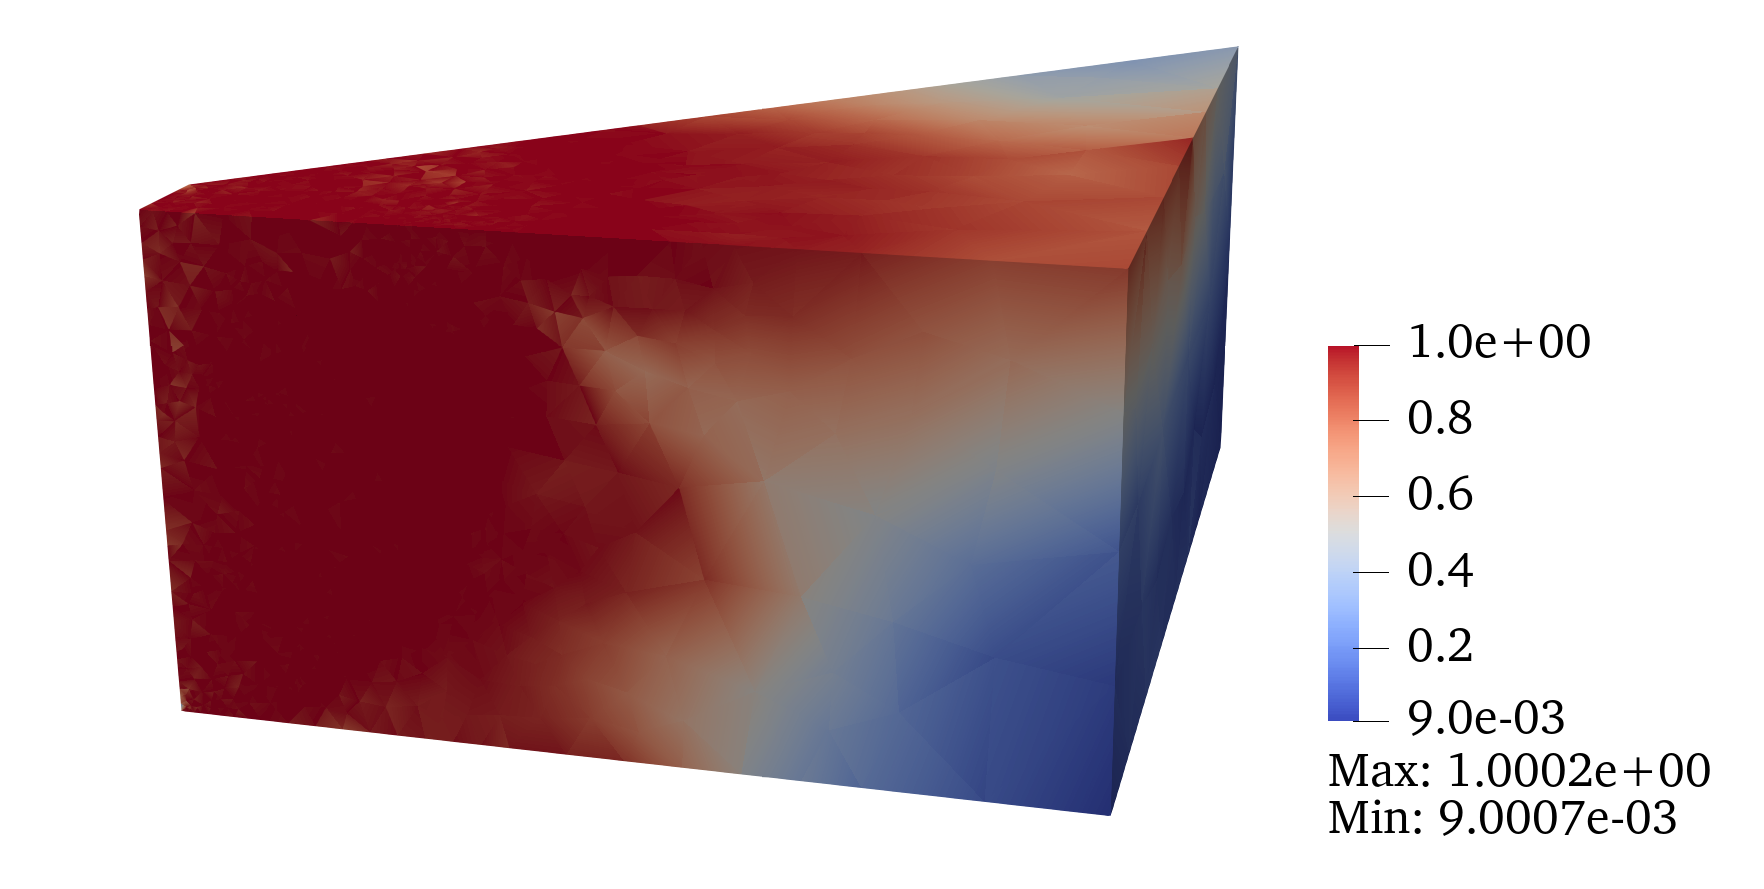
\includegraphics[width=0.55\textwidth]{figures/Res_To_Date/3DVC_solution.png}
  \caption{3D vertical cut problem. \textbf{Left}: physical configuration; \textbf{Right}: solution of the yield function using a refined mesh}
  \label{fig:3DVC_CS}
\end{figure}


\paragraph{Adaptive Mesh Solution}
Adaptive mesh refinement enables the failure mechanism of the vertical cut to be resolved in greater detail. Figure~\ref{fig:3DVC_AMR} presents the corresponding adaptive mesh in wireframe form. For the formulation employing linear stress elements, the best load multiplier obtained is $\beta = 6.55712$. The failure zone is clearly captured by the highly refined red region adjacent to the vertical excavation.

\begin{figure}[htbp]
  \centering
  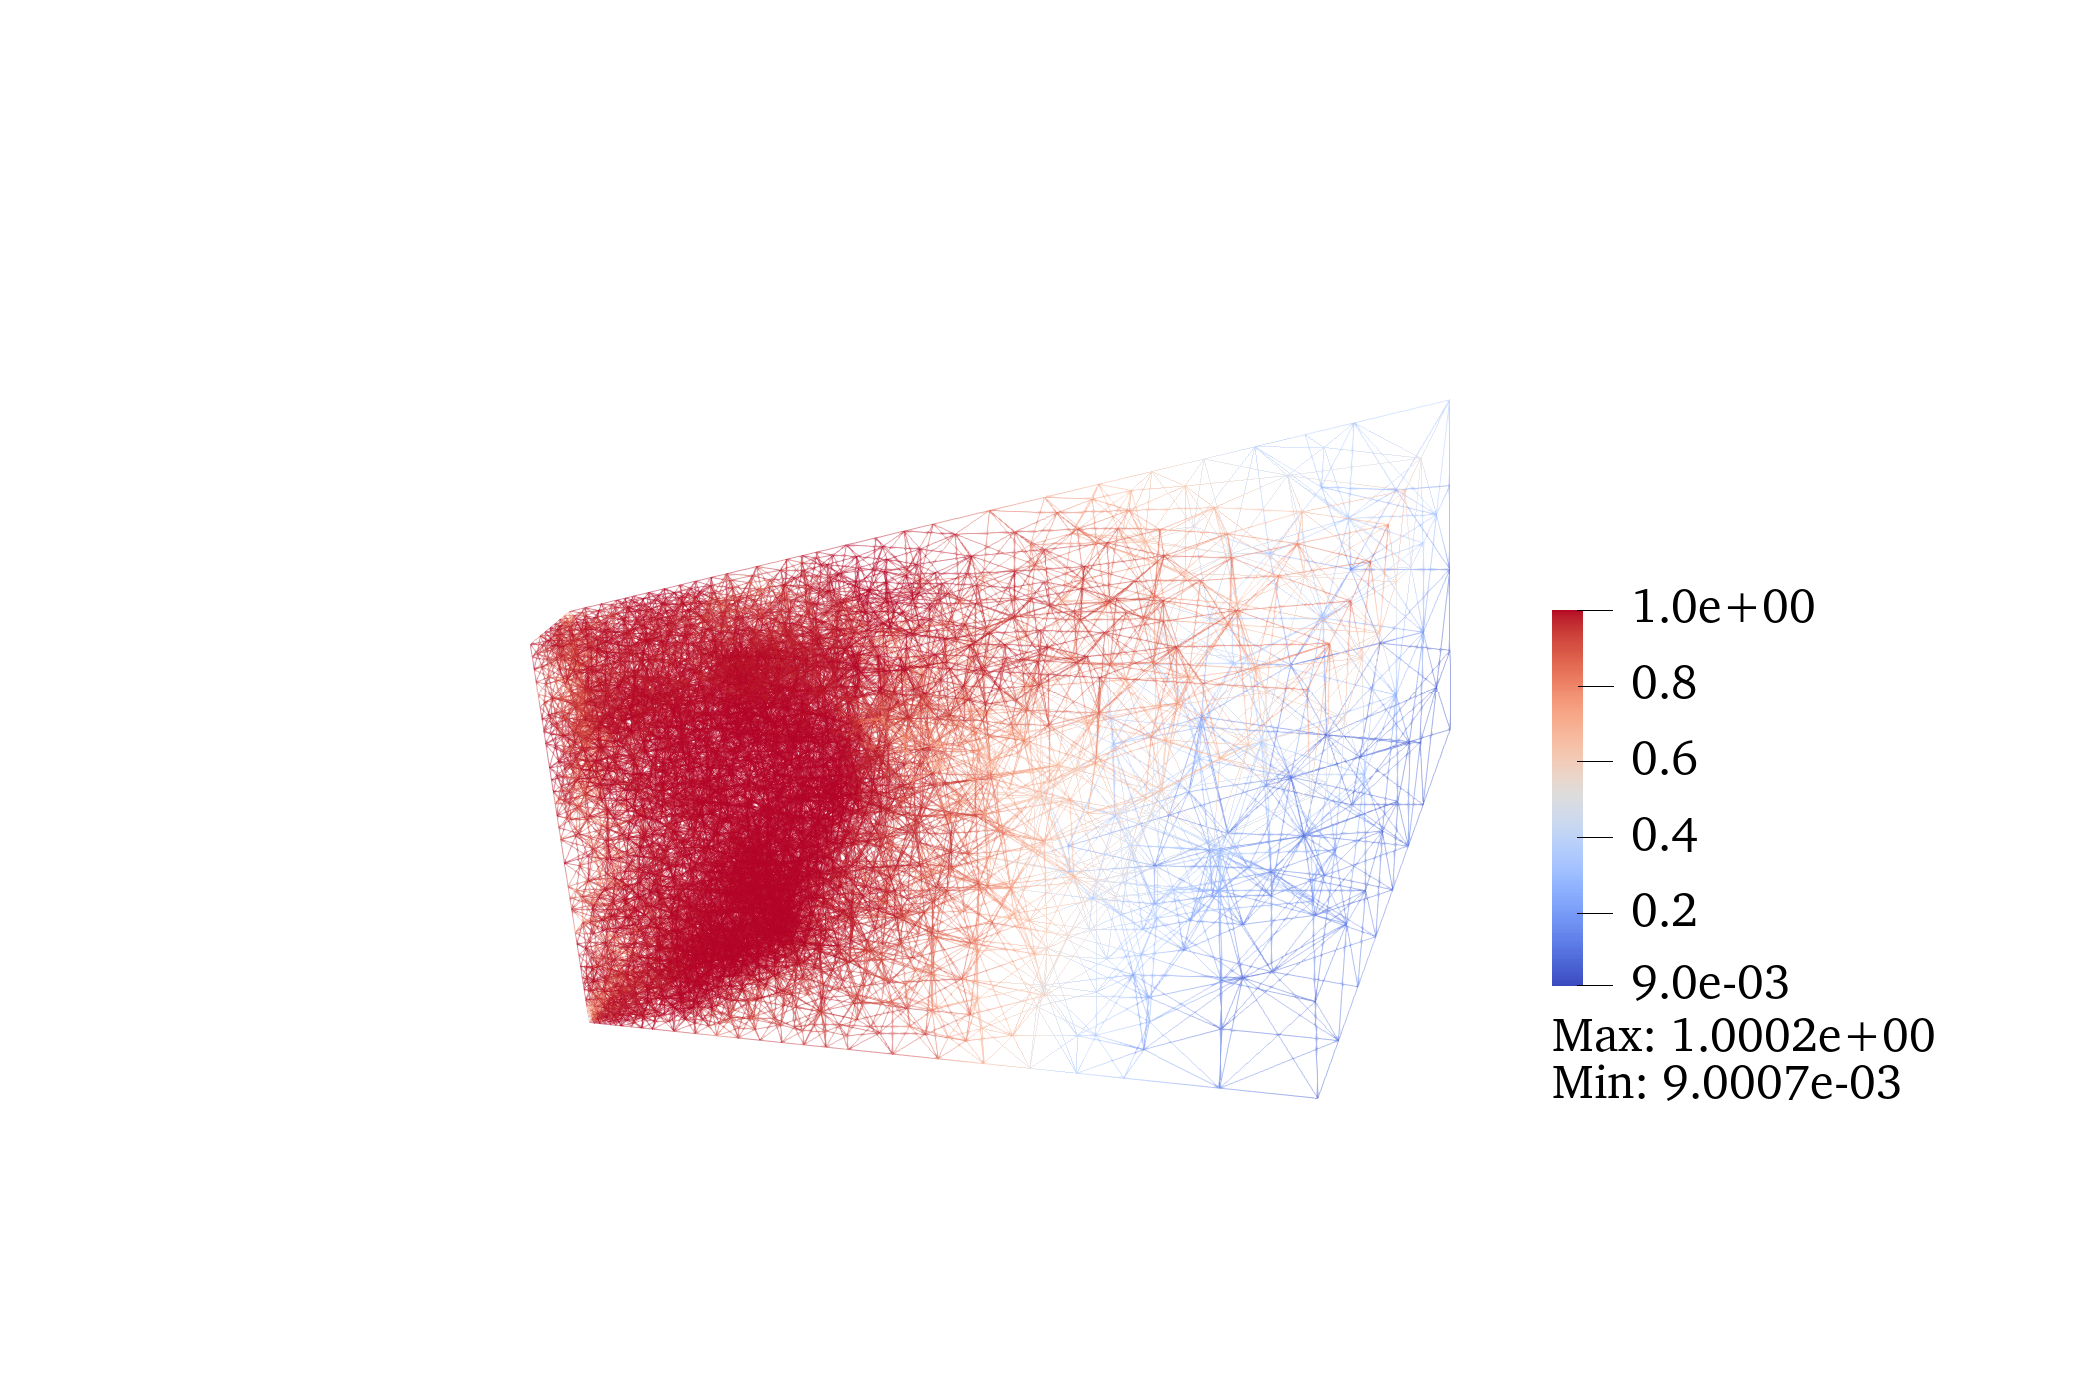
\includegraphics[width=0.8\textwidth]{figures/Res_To_Date/3DVC_AMR_Mesh.png}
  \caption{AMR result of the vertical cut problem in 3D}
  \label{fig:3DVC_AMR}
\end{figure}
\subsubsection{Discussion}

As in the 2D examples, the proposed ADMM solver remains computationally competitive in the 3D benchmarks. Although the speedup over the IPM solvers is generally less pronounced than in 2D, the computational cost per ADMM iteration remains substantially lower than that of an IPM iteration. Moreover, with warm-starting and active-cone identification, the number of ADMM iterations varies only moderately as the problem size increases.

The reduced speedup observed in 3D is not primarily caused by a deterioration of the ADMM iteration itself. Instead, the dominant computational cost shifts increasingly toward the sparse linear algebra, particularly numerical factorization and repeated triangular solves. This effect is much more pronounced in three-dimensional FELA because of the denser connectivity and greater fill-in generated during factorization. The underlying scalability implications are discussed in detail in Section~\ref{sec:3D_scalability}.

To further examine how the individual solver enhancements contribute to the overall performance in 3D, we consider the rigid platen benchmark with a structured mesh of 48,000 linear tetrahedral stress elements and approximately 1.15 million variables. A vanilla GPU-accelerated ADMM implementation already benefits from inexpensive repeated iterations through factorization reuse, while the proposed framework introduces additional mechanisms to improve convergence and reduce the cost of the underlying linear algebra. We therefore compare several solver configurations involving warm-starting (WS), active-cone identification (CI), augmented (AUG) and condensed linear-system formulations, and the alternative ellipsoidal projection strategy. The corresponding results are summarized in Table~\ref{tab:Ablation_table}.


\begin{table}[htbp]
\centering
\caption{Solver performance with different solver options}
\label{tab:Ablation_table}
\begin{tabular}{@{}p{3cm}p{1.8cm}p{1.6cm}p{2cm}p{2.5cm}p{1.4cm}@{}}
\toprule
\textbf{Solver options} & \textbf{Solve time (s)} & \textbf{Iterations} &  \textbf{Analysis time (s)} & \textbf{Factorization time (s)} & \textbf{$\beta$} \\
\midrule
\texttt{AUG + Projection} 	& 41.30  	& 140 	& 19.20 & 18.31 & 2.09477 \\
\texttt{AUG + WS + CI}    	& 61.99  	& 180	& 19.58 & 16.21 & 2.09708 \\
\texttt{AUG + CI}         	& 110.74	& 280 	& 19.82 & 16.01 & 2.09229 \\
\texttt{AUG + WS}         	& 98.34  	& 600 	& 19.96 & 16.09 & 2.09750 \\
\texttt{Condensed}        	& 352.05   & 440  	& 37.35 & 45.00 & 2.09749 \\

\bottomrule
\end{tabular}
\vspace{0.5em}
\end{table}

The individual effects of warm-starting and active-cone identification are evident from the comparison between AUG+WS, AUG+CI, and AUG+WS+CI. Warm-starting alone requires 600 iterations, whereas active-cone identification reduces this to 280 iterations, indicating that CI is particularly effective in accelerating the later stages of convergence. However, CI changes the entries of the system matrix and therefore introduces repeated numerical refactorizations. Consequently, despite the lower iteration count, AUG+CI requires 110.74s, compared with 98.34s for AUG+WS. Combining the two strategies provides a better balance between convergence acceleration and refactorization overhead, reducing the iteration count further to 180 and the total solution time to 61.99s.

The alternative ellipsoidal projection strategy provides a further reduction in computational cost for this particular 3D problem. Compared with AUG+WS+CI, the projection-based formulation reduces the number of iterations from 180 to 140 and the total solution time from 61.99s to 41.30s. However, this improvement is accompanied by a slightly larger discrepancy in the computed collapse multiplier, with $\beta=2.09477$ compared with $\beta=2.09708$ for AUG+WS+CI. Although the difference remains small, the AUG+WS+CI configuration provides a more consistent balance between computational efficiency and solution accuracy. For this reason, AUG+WS+CI is adopted as the default configuration in the remaining 3D benchmark comparisons.

The choice of linear-system formulation has an even stronger influence on the computational cost in 3D. The condensed formulation (with warm-starting and cone identification) requires 352.05s, substantially longer than the augmented configurations, and also incurs markedly larger analysis and factorization costs. Unlike the convergence enhancements discussed above, this difference originates primarily from the sparse linear algebra rather than from the number of ADMM iterations. Indeed, the condensed formulation converges in 440 iterations, fewer than the 600 iterations required by the AUG+WS configuration, yet still takes substantially longer to solve. Forming and factorizing the condensed system generates substantially more fill-in in the 3D problem, increasing both memory consumption and the cost of each repeated triangular solves. This observation motivates the more detailed discussion of the 3D direct-factorization bottleneck in Section~\ref{sec:3D_scalability}.

The use of adaptive mesh refinement also yields tighter lower-bound solutions and provides a more detailed representation of the localized failure region. However, in the present 3D implementation, further refinement is ultimately constrained by the memory demand of sparse direct factorization. This observation reinforces the need for more memory-scalable linear-solver strategies in large-scale 3D FELA.



\section{Discussion}

\subsection{Sources of computational efficiency}

The numerical results indicate that the computational advantage of the proposed framework arises from exploiting the structure of lower-bound FELA at several computational levels.

At the linear-algebra level, the repeated linear systems arising in ADMM permit expensive sparse factorizations to be reused across iterations, resulting in a substantially lower cost per iteration than that of the IPM solvers. At the conic-constraint level, active-cone identification exploits the fact that only a subset of the local yield constraints governs the solution near collapse, allowing the penalty weights to be adapted selectively. At the mesh-sequence level, coarse-to-fine warm-starting transfers information between closely related FELA problems and reduces the transient phase of convergence. Finally, the dominant linear algebra, projection, and vector operations are mapped onto the GPU, further reducing the cost of each ADMM iteration.

These mechanisms are complementary. Warm-starting primarily improves the initial iterate, active-cone identification improves convergence during the later stages of the solve, and GPU acceleration reduces the computational cost of carrying out each iteration. The combined effect is therefore a large reduction in overall time-to-solution especially as the problem size increases.

\subsection{Scalability bottleneck of direct factorization in 3D}
\label{sec:3D_scalability}

The principal scalability limitation of the current 3D implementation arises from fill-in during sparse direct factorization. Although the ADMM iterations remain relatively inexpensive in terms of iteration count, the linear systems generated by three-dimensional FELA become substantially more demanding as the mesh is refined. This behaviour is primarily associated with the different sparsity structure of the 3D formulation.

In lower-bound FELA, the 3D discretization introduces stronger and more spatially extensive coupling than its 2D counterpart. Each stress point contains more stress components, the intra-element equilibrium conditions increase from two equations per stress point in 2D to three in 3D, and the dimension of the SOC blocks increases from three to six for the Drucker--Prager or von Mises formulations considered here. Together with the increased connectivity of three-dimensional finite-element meshes, these larger local blocks lead to a more strongly coupled constraint matrix, as illustrated by the sparsity patterns in Figure~\ref{fig:A_sparsity}.

\begin{figure}
    \centering
    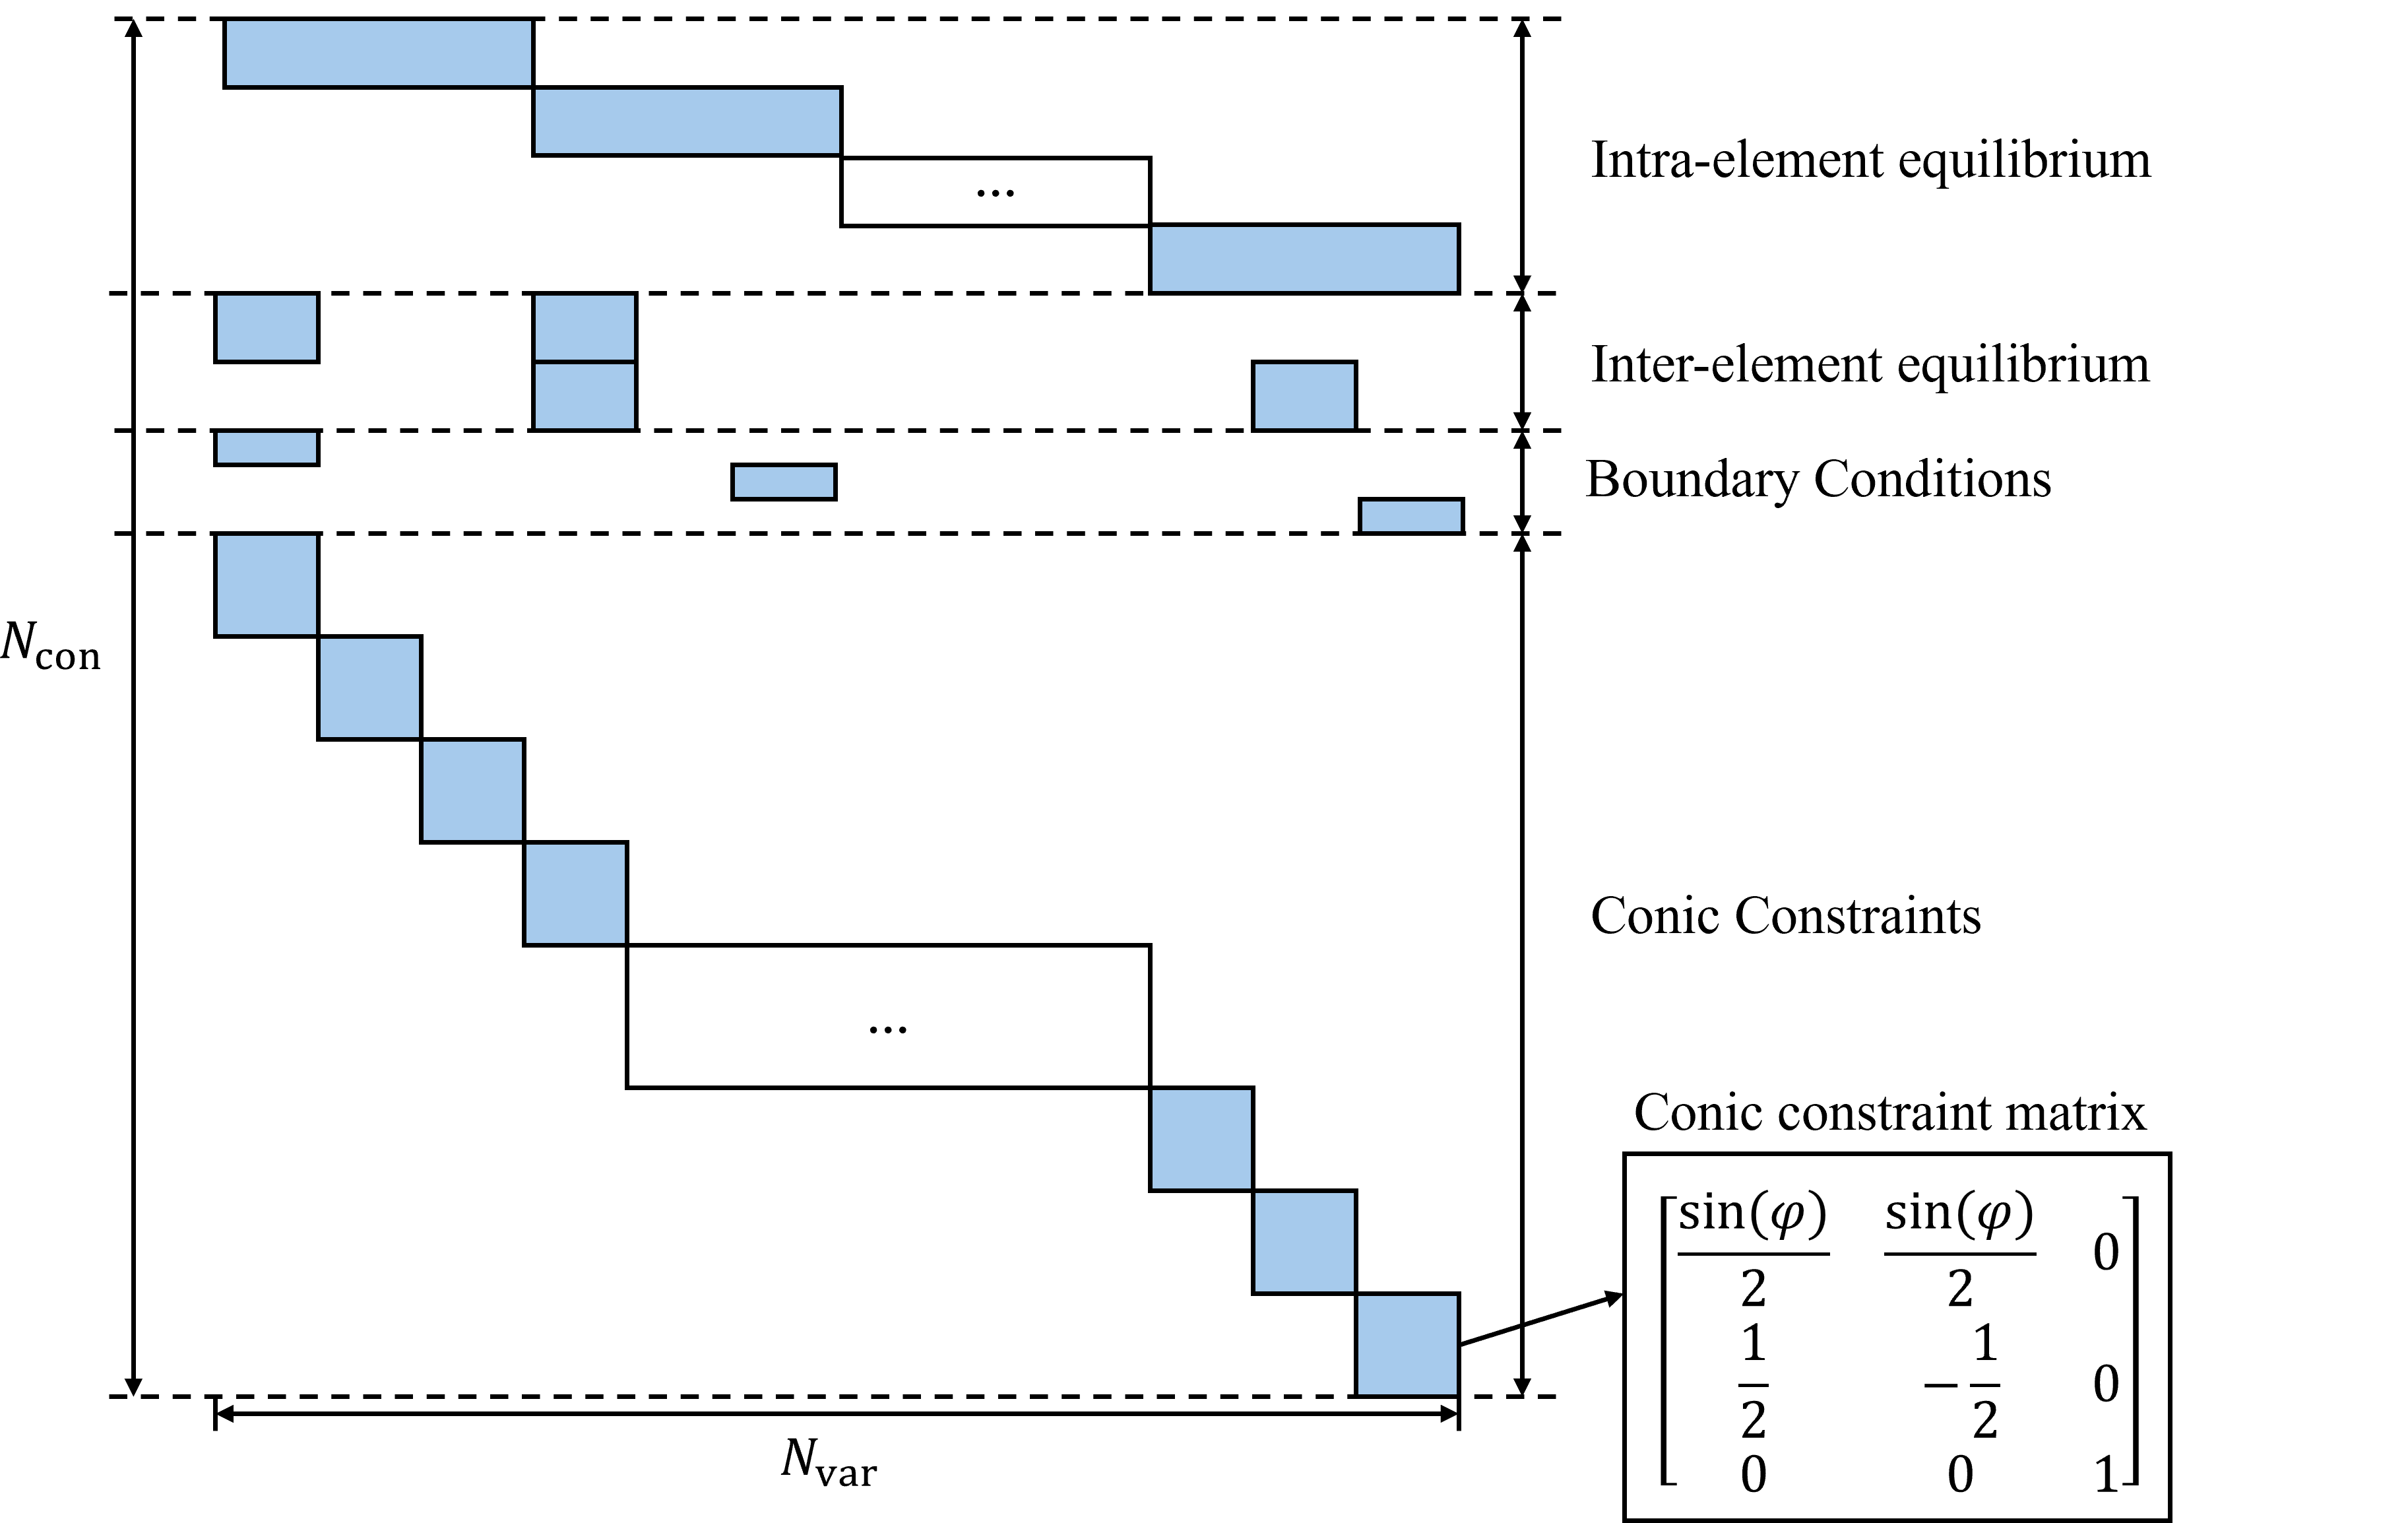
\includegraphics[width=0.8\textwidth]{figures/Res_To_Date/A_sparsity.png}
    \caption{Sparsity patterns of the constraint matrix $A$ in the 2D and 3D FELA formulations.}
    \label{fig:A_sparsity}
\end{figure}

The stronger coupling in the 3D system leads to substantially more fill-in during reordering and factorization. As a result, the numerical factors become significantly larger, increasing both the memory required to store them and the computational cost of the associated sparse linear algebra. In particular, the numerical factorization required whenever the system matrix is updated becomes more expensive, while the repeated triangular solves performed at each ADMM iteration also incur a higher cost.

Consequently, the computational expense of large 3D problems is not determined solely by the number of ADMM iterations. As the factors grow and approach the available GPU memory capacity, memory traffic, data movement, and the cost of operating on the enlarged sparse factors increasingly dominate the overall solution time. This effect can be substantial even when the 2D and 3D problems contain a comparable number of optimization variables, since sparse-factorization cost depends strongly on the sparsity pattern and the resulting fill-in rather than on the system dimension alone.

This explains why the direct GPU-based approach remains highly efficient for the 2D plane-strain benchmarks considered here, while its scalability becomes increasingly constrained by sparse direct factorization in large-scale 3D discretizations. The observed bottleneck therefore motivates the consideration of indirect or matrix-free linear-solver strategies, as discussed in the following section.

\subsection{Potential of indirect and matrix-free ADMM solvers}


Nevertheless, a more scalable direction may be to avoid explicitly computing and storing the sparse factorization altogether, and instead adopt an indirect linear solution strategy within ADMM. This is especially relevant for three-dimensional FELA, where direct factorization of sparse matrices can quickly become unfavourable due to excessive fill-in~\cite{Shewchuk_CG}. As noted in the broader numerical linear algebra literature, iterative solvers are often preferable, and in many large-scale three-dimensional applications practically necessary, due to the memory and computational costs associated with sparse direct methods~\cite{Saad_book}. Several ADMM-based solvers already provide indirect linear-system solvers~\cite{SCS, OSQP, COSMO, GeNIOS}. Notably, SCS has reported speedups from its GPU-based indirect implementation on large-scale problems~\cite{SCS}, suggesting that the combination of ADMM and indirect solves can be practical and scalable for sufficiently large instances.


\subsection{Generality, limitations, and future extensions}

The proposed method achieves a speedup over the IPM on many large-scale problems arising in FELA, while maintaining accuracy comparable to MOSEK under a similar accuracy target. We note, however, that part of this speedup is achieved using a GPU-based implementation, whereas MOSEK is run on a multi-threaded CPU. 

While the proposed acceleration techniques are developed in the context of LB-FELA, they target generic bottlenecks of first-order methods for SOCPs. Therefore, they may also benefit other sparse SOCPs with PDE-like structures. A systematic evaluation on broader classes of problems is left for future work.


Apart from the GPU-accelerated ADMM solver itself, the integration with adaptive mesh refinement enables the computational effort to be concentrated in the regions most relevant to the collapse mechanism, leading to tighter lower-bound solutions without uniformly refining the entire domain.

Future work will also consider more advanced yield criteria, such as Mohr-Coulomb and Lade-Duncan. Incorporating these criteria would increase the practical value of the proposed methodology, as they are widely used in geotechnical and engineering applications. Within the ADMM framework, such criteria can be incorporated provided that the projection of a general stress state onto the admissible yield surface can be computed efficiently~\cite{daSilva_2020, 3DLD}. For example, although not necessarily in the context of FELA, Clausen and co-workers implemented the three-dimensional Mohr-Coulomb criterion using a return-mapping strategy, in which the stress state is transformed into principal stress space, projected onto the yield surface, and then transformed back to the original stress space~\cite{Clausen_2007}. Extending this type of projection strategy to the present FELA-ADMM framework is a promising direction for future research.







\section{Conclusion}

This paper presents a scalable GPU-accelerated ADMM framework for lower-bound finite element limit analysis. By leveraging ADMM together with tailored acceleration strategies, the proposed method provides an efficient solution pipeline for large-scale FELA problems. The framework is validated systematically on 2D benchmark problems and further extended to representative 3D applications.

Across the considered benchmarks, the proposed solver delivers substantial reductions in time-to-solution relative to a state-of-the-art interior-point solver, while maintaining essentially identical LB collapse multipliers. In particular, the numerical results demonstrate that the speedups are achieved without sacrificing solution quality, supporting the use of the proposed approach as a practical alternative for large-scale conic optimization problems. Combined with adaptive mesh refinement, the solver is able to obtain a tight, strict LB solution of a large-scale 2D problem on a modest GPU. Representative 3D benchmarks show that the proposed solver remains computationally effective beyond the 2D setting, while large-scale adaptive mesh refinement simulations further highlight its scalability and practical applicability. Together, these results indicate that the proposed method combines strong performance in 2D with promising extensibility to 3D lower-bound FELA.

In addition, the integration of adaptive mesh refinement (AMR) and Bernstein elements further improves the quality of the computed strict lower bound, enabling high-quality solutions to be obtained efficiently for challenging geometries and complex geotechnical stress fields. The projection-based formulation also highlights the flexibility of the proposed ADMM framework, indicating its potential to accommodate more sophisticated yield criteria within the same computational pipeline.

Overall, the combination of scalable conic optimization, GPU acceleration, mesh adaptivity, and higher-order elements provides an effective workflow toward high-fidelity limit analysis at problem sizes that are difficult to handle with conventional second-order methods.





%% Labels are used to cross-reference an item using \ref command.


\bibliographystyle{elsarticle-num}
\bibliography{citations}




\end{document}

\endinput
%%
%% End of file `elsarticle-template-num.tex'.
